%
% GD2 cookbook
%

%\documentclass[letterpaper, 10 pt, conference]{ieeeconf}  % Comment this line out
                                                          % if you need a4paper
%\documentclass[onecolumn,a4paper, 10pt, conference]{ieeeconf}      % Use this line for a4
\documentclass[10pt]{book}

\usepackage[paperwidth=6.69in, paperheight=9.61in]{geometry}

% \usepackage[T1]{fontenc}
% \usepackage[scaled]{helvet}
% \renewcommand*\familydefault{\sfdefault}

\usepackage{charter}

% \usepackage[T1]{fontenc}
% \usepackage[urw-garamond]

% See the \addtolength command later in the file to balance the column lengths
% on the last page of the document

\usepackage{makeidx}         % allows index generation
\makeindex
\usepackage{graphicx}        % standard LaTeX graphics tool
                             % when including figure files
\usepackage{multicol}        % used for the two-column index
% \usepackage[bottom]{footmisc}% places footnotes at page bottom
\usepackage{amsmath}
\usepackage{longtable}
\usepackage{color}
\usepackage{fancyvrb}
\usepackage{rotating}
\usepackage{supertabular}
\usepackage{url}
\usepackage{array}
\usepackage{verbatim}
\usepackage{setspace}
\usepackage[]{caption}
\usepackage{listings}
\usepackage{wrapfig}
\usepackage{framed}
\usepackage{alltt}
\captionsetup{font=small}

% The following packages can be found on http:\\www.ctan.org
\usepackage{graphics} % for pdf, bitmapped graphics files
\usepackage{epsfig} % for postscript graphics files
\usepackage{tikz}
\usetikzlibrary{arrows,decorations.pathmorphing,backgrounds,positioning,fit,petri,shapes.misc}
\usepackage[linkbordercolor={.9 .9 .9}]{hyperref}

\usepackage[dotinlabels]{titletoc}

\newlength\widest
\settowidth\widest{99.99.}

\titlecontents{section}[1pc]
{\addvspace{0pc}}
{\parbox[t]{\widest}{\hfill\thecontentslabel.}
\hspace{3mm}}
{}
{\normalsize\titlerule*[6pt]{.}\contentspage}
[\addvspace{0pt}]

% Customizations for this document only
\definecolor{light-gray}{gray}{0.90}

\newcommand{\gdtwo}{Gameduino 2 }
\newcommand{\gdtwos}{Gameduino 2's }
\newcommand{\itwoc}{I$^{\textrm{2}}$C }
\newcommand{\sqmm}{mm$^{\textrm{2}}$}

\newcommand{\png}[1]{
\begin{center}
\includegraphics[width=0.8\textwidth]{assets/#1.png}
\end{center}
}

\newcommand{\szpng}[2]{
\begin{center}
\includegraphics[width=#1\textwidth]{assets/#2.png}
\end{center}
}

\newcommand{\minipng}[1]{
\begin{center}
\includegraphics[width=0.4\textwidth]{assets/#1.png}
\end{center}
}

\newcommand{\mach}[1]{\texttt{\textbf{#1}}}

\newcommand{\defidx}[1]{
\index{#1@\mach{#1}}
}
\newcommand{\cmdidx}[1]{
\index{#1@\mach{#1()}}
}
\newcommand{\cmd}[1]{\cmdidx{cmd\_#1}\nameref{cmd:#1}}
\newcommand{\dcmd}[1]{\cmdidx{#1}\nameref{#1}}

\newcommand{\xref}[1]{\textit{\nameref{#1}} on  p.\pageref{#1}}

\newcommand{\boldindex}[1]{\textbf{\hyperpage{#1}}}

\newcommand{\term}[1]{\emph{#1}\index{#1}}


\makeatletter
\def\PY@reset{\let\PY@it=\relax \let\PY@bf=\relax%
    \let\PY@ul=\relax \let\PY@tc=\relax%
    \let\PY@bc=\relax \let\PY@ff=\relax}
\def\PY@tok#1{\csname PY@tok@#1\endcsname}
\def\PY@toks#1+{\ifx\relax#1\empty\else%
    \PY@tok{#1}\expandafter\PY@toks\fi}
\def\PY@do#1{\PY@bc{\PY@tc{\PY@ul{%
    \PY@it{\PY@bf{\PY@ff{#1}}}}}}}
\def\PY#1#2{\PY@reset\PY@toks#1+\relax+\PY@do{#2}}

\expandafter\def\csname PY@tok@gd\endcsname{\def\PY@tc##1{\textcolor[rgb]{0.63,0.00,0.00}{##1}}}
\expandafter\def\csname PY@tok@gu\endcsname{\let\PY@bf=\textbf\def\PY@tc##1{\textcolor[rgb]{0.50,0.00,0.50}{##1}}}
\expandafter\def\csname PY@tok@gt\endcsname{\def\PY@tc##1{\textcolor[rgb]{0.00,0.27,0.87}{##1}}}
\expandafter\def\csname PY@tok@gs\endcsname{\let\PY@bf=\textbf}
\expandafter\def\csname PY@tok@gr\endcsname{\def\PY@tc##1{\textcolor[rgb]{1.00,0.00,0.00}{##1}}}
\expandafter\def\csname PY@tok@cm\endcsname{\let\PY@it=\textit\def\PY@tc##1{\textcolor[rgb]{0.25,0.50,0.50}{##1}}}
\expandafter\def\csname PY@tok@vg\endcsname{\def\PY@tc##1{\textcolor[rgb]{0.10,0.09,0.49}{##1}}}
\expandafter\def\csname PY@tok@m\endcsname{\def\PY@tc##1{\textcolor[rgb]{0.40,0.40,0.40}{##1}}}
\expandafter\def\csname PY@tok@mh\endcsname{\def\PY@tc##1{\textcolor[rgb]{0.40,0.40,0.40}{##1}}}
\expandafter\def\csname PY@tok@go\endcsname{\def\PY@tc##1{\textcolor[rgb]{0.53,0.53,0.53}{##1}}}
\expandafter\def\csname PY@tok@ge\endcsname{\let\PY@it=\textit}
\expandafter\def\csname PY@tok@vc\endcsname{\def\PY@tc##1{\textcolor[rgb]{0.10,0.09,0.49}{##1}}}
\expandafter\def\csname PY@tok@il\endcsname{\def\PY@tc##1{\textcolor[rgb]{0.40,0.40,0.40}{##1}}}
\expandafter\def\csname PY@tok@cs\endcsname{\let\PY@it=\textit\def\PY@tc##1{\textcolor[rgb]{0.25,0.50,0.50}{##1}}}
\expandafter\def\csname PY@tok@cp\endcsname{\def\PY@tc##1{\textcolor[rgb]{0.74,0.48,0.00}{##1}}}
\expandafter\def\csname PY@tok@gi\endcsname{\def\PY@tc##1{\textcolor[rgb]{0.00,0.63,0.00}{##1}}}
\expandafter\def\csname PY@tok@gh\endcsname{\let\PY@bf=\textbf\def\PY@tc##1{\textcolor[rgb]{0.00,0.00,0.50}{##1}}}
\expandafter\def\csname PY@tok@ni\endcsname{\let\PY@bf=\textbf\def\PY@tc##1{\textcolor[rgb]{0.60,0.60,0.60}{##1}}}
\expandafter\def\csname PY@tok@nl\endcsname{\def\PY@tc##1{\textcolor[rgb]{0.63,0.63,0.00}{##1}}}
\expandafter\def\csname PY@tok@nn\endcsname{\let\PY@bf=\textbf\def\PY@tc##1{\textcolor[rgb]{0.00,0.00,1.00}{##1}}}
\expandafter\def\csname PY@tok@no\endcsname{\def\PY@tc##1{\textcolor[rgb]{0.53,0.00,0.00}{##1}}}
\expandafter\def\csname PY@tok@na\endcsname{\def\PY@tc##1{\textcolor[rgb]{0.49,0.56,0.16}{##1}}}
\expandafter\def\csname PY@tok@nb\endcsname{\def\PY@tc##1{\textcolor[rgb]{0.00,0.50,0.00}{##1}}}
\expandafter\def\csname PY@tok@nc\endcsname{\let\PY@bf=\textbf\def\PY@tc##1{\textcolor[rgb]{0.00,0.00,1.00}{##1}}}
\expandafter\def\csname PY@tok@nd\endcsname{\def\PY@tc##1{\textcolor[rgb]{0.67,0.13,1.00}{##1}}}
\expandafter\def\csname PY@tok@ne\endcsname{\let\PY@bf=\textbf\def\PY@tc##1{\textcolor[rgb]{0.82,0.25,0.23}{##1}}}
\expandafter\def\csname PY@tok@nf\endcsname{\def\PY@tc##1{\textcolor[rgb]{0.00,0.00,1.00}{##1}}}
\expandafter\def\csname PY@tok@si\endcsname{\let\PY@bf=\textbf\def\PY@tc##1{\textcolor[rgb]{0.73,0.40,0.53}{##1}}}
\expandafter\def\csname PY@tok@s2\endcsname{\def\PY@tc##1{\textcolor[rgb]{0.73,0.13,0.13}{##1}}}
\expandafter\def\csname PY@tok@vi\endcsname{\def\PY@tc##1{\textcolor[rgb]{0.10,0.09,0.49}{##1}}}
\expandafter\def\csname PY@tok@nt\endcsname{\let\PY@bf=\textbf\def\PY@tc##1{\textcolor[rgb]{0.00,0.50,0.00}{##1}}}
\expandafter\def\csname PY@tok@nv\endcsname{\def\PY@tc##1{\textcolor[rgb]{0.10,0.09,0.49}{##1}}}
\expandafter\def\csname PY@tok@s1\endcsname{\def\PY@tc##1{\textcolor[rgb]{0.73,0.13,0.13}{##1}}}
\expandafter\def\csname PY@tok@sh\endcsname{\def\PY@tc##1{\textcolor[rgb]{0.73,0.13,0.13}{##1}}}
\expandafter\def\csname PY@tok@sc\endcsname{\def\PY@tc##1{\textcolor[rgb]{0.73,0.13,0.13}{##1}}}
\expandafter\def\csname PY@tok@sx\endcsname{\def\PY@tc##1{\textcolor[rgb]{0.00,0.50,0.00}{##1}}}
\expandafter\def\csname PY@tok@bp\endcsname{\def\PY@tc##1{\textcolor[rgb]{0.00,0.50,0.00}{##1}}}
\expandafter\def\csname PY@tok@c1\endcsname{\let\PY@it=\textit\def\PY@tc##1{\textcolor[rgb]{0.25,0.50,0.50}{##1}}}
\expandafter\def\csname PY@tok@kc\endcsname{\let\PY@bf=\textbf\def\PY@tc##1{\textcolor[rgb]{0.00,0.50,0.00}{##1}}}
\expandafter\def\csname PY@tok@c\endcsname{\let\PY@it=\textit\def\PY@tc##1{\textcolor[rgb]{0.25,0.50,0.50}{##1}}}
\expandafter\def\csname PY@tok@mf\endcsname{\def\PY@tc##1{\textcolor[rgb]{0.40,0.40,0.40}{##1}}}
\expandafter\def\csname PY@tok@err\endcsname{\def\PY@bc##1{\setlength{\fboxsep}{0pt}\fcolorbox[rgb]{1.00,0.00,0.00}{1,1,1}{\strut ##1}}}
\expandafter\def\csname PY@tok@kd\endcsname{\let\PY@bf=\textbf\def\PY@tc##1{\textcolor[rgb]{0.00,0.50,0.00}{##1}}}
\expandafter\def\csname PY@tok@ss\endcsname{\def\PY@tc##1{\textcolor[rgb]{0.10,0.09,0.49}{##1}}}
\expandafter\def\csname PY@tok@sr\endcsname{\def\PY@tc##1{\textcolor[rgb]{0.73,0.40,0.53}{##1}}}
\expandafter\def\csname PY@tok@mo\endcsname{\def\PY@tc##1{\textcolor[rgb]{0.40,0.40,0.40}{##1}}}
\expandafter\def\csname PY@tok@kn\endcsname{\let\PY@bf=\textbf\def\PY@tc##1{\textcolor[rgb]{0.00,0.50,0.00}{##1}}}
\expandafter\def\csname PY@tok@mi\endcsname{\def\PY@tc##1{\textcolor[rgb]{0.40,0.40,0.40}{##1}}}
\expandafter\def\csname PY@tok@gp\endcsname{\let\PY@bf=\textbf\def\PY@tc##1{\textcolor[rgb]{0.00,0.00,0.50}{##1}}}
\expandafter\def\csname PY@tok@o\endcsname{\def\PY@tc##1{\textcolor[rgb]{0.40,0.40,0.40}{##1}}}
\expandafter\def\csname PY@tok@kr\endcsname{\let\PY@bf=\textbf\def\PY@tc##1{\textcolor[rgb]{0.00,0.50,0.00}{##1}}}
\expandafter\def\csname PY@tok@s\endcsname{\def\PY@tc##1{\textcolor[rgb]{0.73,0.13,0.13}{##1}}}
\expandafter\def\csname PY@tok@kp\endcsname{\def\PY@tc##1{\textcolor[rgb]{0.00,0.50,0.00}{##1}}}
\expandafter\def\csname PY@tok@w\endcsname{\def\PY@tc##1{\textcolor[rgb]{0.73,0.73,0.73}{##1}}}
\expandafter\def\csname PY@tok@kt\endcsname{\def\PY@tc##1{\textcolor[rgb]{0.69,0.00,0.25}{##1}}}
\expandafter\def\csname PY@tok@ow\endcsname{\let\PY@bf=\textbf\def\PY@tc##1{\textcolor[rgb]{0.67,0.13,1.00}{##1}}}
\expandafter\def\csname PY@tok@sb\endcsname{\def\PY@tc##1{\textcolor[rgb]{0.73,0.13,0.13}{##1}}}
\expandafter\def\csname PY@tok@k\endcsname{\let\PY@bf=\textbf\def\PY@tc##1{\textcolor[rgb]{0.00,0.50,0.00}{##1}}}
\expandafter\def\csname PY@tok@se\endcsname{\let\PY@bf=\textbf\def\PY@tc##1{\textcolor[rgb]{0.73,0.40,0.13}{##1}}}
\expandafter\def\csname PY@tok@sd\endcsname{\let\PY@it=\textit\def\PY@tc##1{\textcolor[rgb]{0.73,0.13,0.13}{##1}}}

\def\PYZbs{\char`\\}
\def\PYZus{\char`\_}
\def\PYZob{\char`\{}
\def\PYZcb{\char`\}}
\def\PYZca{\char`\^}
\def\PYZam{\char`\&}
\def\PYZlt{\char`\<}
\def\PYZgt{\char`\>}
\def\PYZsh{\char`\#}
\def\PYZpc{\char`\%}
\def\PYZdl{\char`\$}
\def\PYZhy{\char`\-}
\def\PYZsq{\char`\'}
\def\PYZdq{\char`\"}
\def\PYZti{\char`\~}
% for compatibility with earlier versions
\def\PYZat{@}
\def\PYZlb{[}
\def\PYZrb{]}
\makeatother



\title{\LARGE \bf
The Gameduino 2 \\
Tutorial, Reference \\
and Cookbook
}

\author{James Bowman \\
	{\tt\small jamesb@excamera.com} \\
  Excamera Labs, \\
  Pescadero CA, \\
  USA
}
\date{}
        
\usepackage[dotinlabels]{titletoc}
\titlecontents{section}[1pc]
{\addvspace{0pc}}
{\thecontentslabel.\hspace{3mm}}
{}
{\normalsize\titlerule*[6pt]{.}\contentspage}
[\addvspace{0pt}]

% \SetWatermarkColor[rgb]{.9,.9,.9}

\begin{document}

\maketitle

%% copyrightpage
\begingroup
\footnotesize
\parindent 0pt
\parskip \baselineskip
\textcopyright{} 2013, James Bowman \\
All rights reserved

%     This work may be distributed and/or modified under the conditions
% of the LaTeX Project Public License, either version~1.3 of this license
% or (at your option) any later version. The latest version is in \\
% \hspace*{2em} \url{http://www.latex-project.org/lppl.txt} \\
% and version~1.3 or later is part of all distributions of LaTeX
% version 2005/12/01 or later.
% 
%     This work has the LPPL maintenance status `maintained'.
% 
%     The Current Maintainer of this work is Peter Wilson.
% 
%     The work consists of the file \texttt{titlepages.tex} and the
% derived file \texttt{titlepages.pdf}.
% 
% The paper used in this publication may meet the minimum 
% requirements of the American National Standard for 
% Information Sciences --- Permanence of Paper for Printed
% Library Materials, ANSI Z39.48--1984.

\begin{center}
\begin{tabular}{ll}
First edition:  & December 2013 \\
\end{tabular}
\end{center}

\vfill

Bowman, James.\\
\hspace*{2em} The Gameduino 2 Tutorial, Reference and Cookbook / James Bowman. -- \\
\hspace*{1em} 1st Excamera Labs ed. \\
\hspace*{2em} 200 p. \hspace*{2em} \\
\hspace*{2em} Includes illustrations, bibliographical references and index. \\
\hspace*{2em} ISBN 978-1492888628 \\
% \hspace*{2em} ISBN XXX-XXXXXXXXXX \\
\hspace*{2em} 1. Microcontrollers -- Programming \hspace*{2em} I. Title


\vfill

% Printed in the World

\endgroup

\thispagestyle{empty}
\pagestyle{headings}

\tableofcontents

\part{Tutorial}

%%%%%%%%%%%%%%%%%%%%%%%%%%%%%%%%%%%%%%%%%%%%%%%%%%%%%%%%%%%%%%%%%%%%%%%%
\chapter{Plug in. Power up. Play something}

\begin{center}
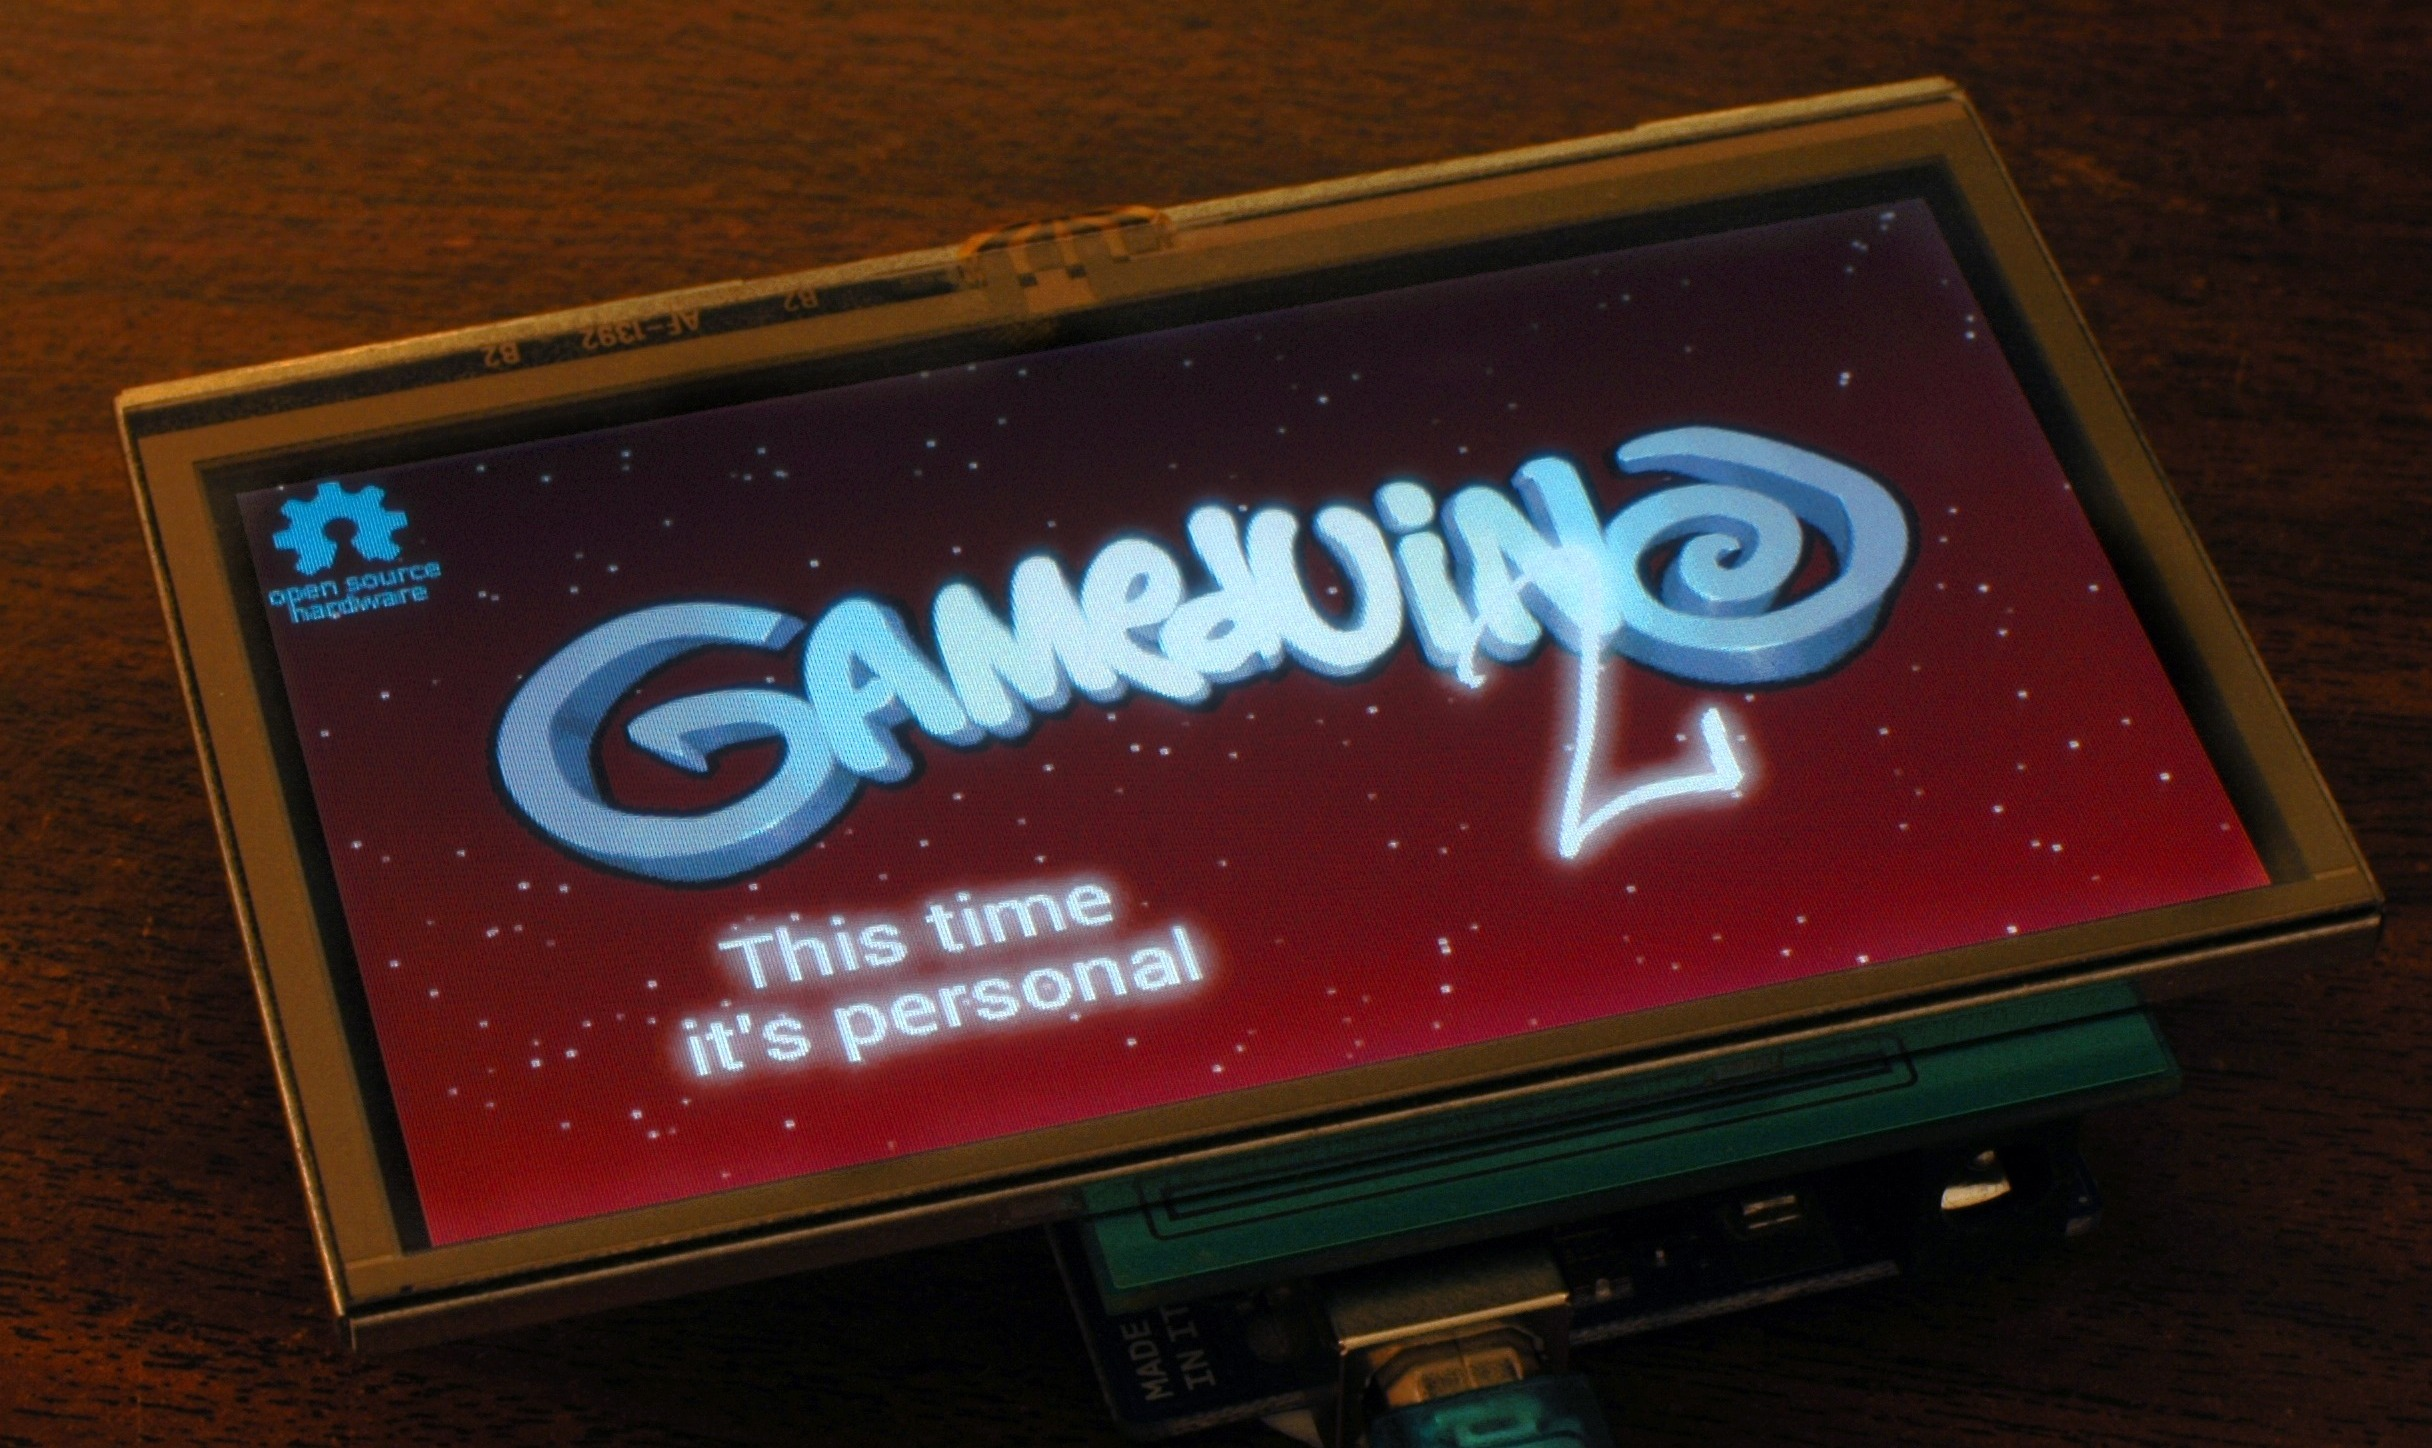
\includegraphics[width=0.9\textwidth]{assets/plugin.jpg}
\end{center}

\begin{enumerate}

\item
Download the \gdtwo library \mach{Gameduino2.zip} from \\
\url{http://gameduino.com/code} and install it in the Arduino IDE.
Instructions for doing this are at
\url{http://arduino.cc/en/Guide/Libraries}.

\item
Attach \gdtwo to the Arduino, making sure that the pins are aligned properly,
and that none are bent.

\item
Power up the Arduino. Nothing will appear on the \gdtwo screen until a sketch is loaded on the Arduino.

\item
Restart the Arduino IDE, and load one of the sketches, for example \\
\begin{small}
\mach{File} $\triangleright$
\mach{Sketchbook} $\triangleright$
\mach{libraries} $\triangleright$
\mach{Gameduino2} $\triangleright$
\mach{1.Basics} $\triangleright$
\mach{helloworld}
\end{small}

\begin{center}
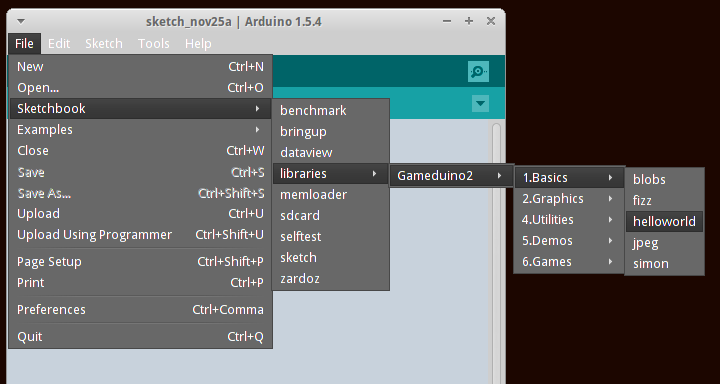
\includegraphics[width=1.0\textwidth]{assets/menu.png}
\end{center}

\item
Compile and download the sketch to the Arduino.
\gdtwo should start up and run the sketch.

\item
Many of the examples use data files from the microSD card.
To run them, format a microSD card and copy the files
from \mach{Gameduino2sd.zip} (also at \url{http://gameduino.com/code})
onto it.

\item
Enjoy!

\end{enumerate}

%%%%%%%%%%%%%%%%%%%%%%%%%%%%%%%%%%%%%%%%%%%%%%%%%%%%%%%%%%%%%%%%%%%%%%%%
\chapter{Quick start}

This chapter introduces the basics of \gdtwo -
from ``hello world'' to creating a simple touch-based game.

\newcommand*\cleartoleftpage{%
  \clearpage
    \ifodd\value{page}\hbox{}\newpage\fi
    }

\cleartoleftpage
\section{Hello world}
\label{helloworld}
\index{drawing!text}
\index{text, drawing}
\index{demos!hello world}

\png{helloworld}

\newcommand{\eg}[1]{
\begin{framed}
\input{code/#1.inc}
\end{framed}
}

\eg{helloworld-A}

The code in \mach{loop()} clears the screen to a relaxing deep green color, then writes the text centered on the screen.
This code runs continuously, redrawing the screen 60 times every second.
Because the same image is being drawn every time, the screen does not move.

\dcmd{ClearColorRGB} is a drawing command: it sets the color used for screen clears.
Here the color is \texttt{0x103000}, a dark green.
Gameduino 2 uses standard hex triplets for colors, like HTML.
\index{HTML color triplet}

\dcmd{Clear} is another drawing command.
It clears the screen to the dark green color.
Drawing must always begin with a clear screen.

\cmd{text} is a higher-level GPU command.
It draws a text string in a particular font on the screen. 
In this case the text is being drawn in the center of the screen, at $(x,y)$ coordinates (240, 136).
\mach{OPT\_CENTER} draws the text so that its center is at (240, 136).
The font number 31 is the largest available built-in font.

Finally, \mach{GD.swap()} tells the graphics system that the drawing is finished
and it can be made visible on the screen.
There are always two copies of the screen: one that is visible, and one that is work-in-progress.
Calling \mach{GD.swap()} exchanges the screens so that the work-in-progress screen becomes visible.
This swapping system (sometimes called \term{double buffering}) means that the display updates smoothly,
only updating when the program calls \mach{GD.swap()}.

\index{screen coordinates}
\index{coordinates, screen}
Gameduino 2's screen is 480 pixels wide and 272 high.
$(0,0)$ is the top-left corner of the screen, $(479,271)$ is the bottom right.
The center pixel on the screen is at $(240,136)$.

\begin{center}
\begin{tikzpicture}
    [align=center,node distance=4cm]
    \node [opacity=0.2,inner sep=0] at (0,0) (png) {
\includegraphics[width=0.8\textwidth]{assets/helloworld.png}};

    \node [below of=png] (240x136) {$x=240,y=136$)};
    \draw [-latex]   (240x136) -- (png.center);

    \draw [-latex]   (png.north west) -- (png.north east)
      node[above left,pos=0] {$x=y=0$}
      node[above] {$x=480$};
    \draw [-latex]   (png.north west) -- (png.south west)
      node[left] {$y=272$};

\end{tikzpicture}
\end{center}

\newpage
\section{Circles are large points}
\index{points} \index{circles}
\defidx{POINTS}
\index{drawing!points}
\index{points}

What about graphics?
Graphics drawing uses two commands:
\dcmd{Begin} and \dcmd{Vertex2ii}.
\dcmd{Begin} tells the graphics system what to draw,
and \dcmd{Vertex2ii} draws it.  So this code
draws two single-pixel points, at coordinates (220,100) and (260,170):

\eg{examples-a}

\png{0000}

The \mach{Begin(POINTS)} tells the GPU to start drawing points.
Then each call to \dcmd{Vertex2ii} draws another point at the specified $(x, y)$ screen coordinates.
Note that if you don't supply a \dcmd{Begin},
then the hardware doesn't know what to draw so it ignores the following \dcmd{Vertex2ii} calls.

\newpage
The GD library also has a
\dcmd{PointSize} call that lets you set the size of points.
Its argument is the radius of the points, in units of $1/16$th of a pixel.
The hardware uses these \term{subpixel} units to give you fine control over the
dimensions of drawn objects, much finer than the width of a pixel.
For situations where you want to specify a distance in pixels, it is usually clearest to multiply the distance by 16 in the code.

Adding a call to \dcmd{PointSize} before the drawn points
gives huge points with a radius of 30 pixels (and hence a \term{diameter} of 60 pixels).

\png{0001}
\eg{examples-b}


In fact, the hardware always draws \mach{POINTS} using mathematical circles, but when the point size is small the circles
happen to look like single pixels.

\end{samepage}

\newpage
\section{Color and transparency}

Adding calls to \dcmd{ColorRGB} before each vertex changes their colors to
orange and teal:

\png{0002}
\eg{examples-c}

\dcmd{ClearColorRGB}, \dcmd{ColorRGB} and \dcmd{PointSize} are examples of \term{graphics state},
like variables in the graphics hardware.
When changed by program, they will affect later drawing operations.
To keep life simple,
all graphics state is set to a default value at the start of the frame.
As you might have already guessed, the default \dcmd{ColorRGB} is white,
which is why ``Hello world'' is white.
The default \dcmd{PointSize} is 8, meaning a radius of half a pixel.

You can also set the transparency of drawing, just like color.
Transparency is controlled by an alpha channel, which has a value from 0 to 255.
\index{alpha}
\index{transparency, alpha}
0 means completely transparent.
255 -- the default -- means completely opaque.
Setting the transparency to 128 with \dcmd{ColorA} before the point drawing
makes the points 50\% transparent.
\png{0003}
\eg{examples-d}

The color commands \dcmd{ColorRGB} and \dcmd{ClearColorRGB} also accept (R,G,B) triplet values.
So \mach{ColorRGB(0x0080ff)} can be written \mach{ColorRGB(0, 128, 255)} instead:

\eg{examples-triplet}

\newpage
\section{Demo: fizz}
\label{fizz}
\index{demos!fizz}

\png{fizz}
\eg{fizz-a}

Every frame, ``fizz'' draws 100 points, with random size, color and transparency.
Because each frame is 1/60th of a second, the effect is a seething frenzy of luridly colored disks.
\index{frenzy, seething}

\begin{center}

\includegraphics[width=0.24\textwidth]{assets/fizz-6.png}

\includegraphics[width=0.24\textwidth]{assets/fizz-7.png}

\includegraphics[width=0.24\textwidth]{assets/fizz-8.png}

\includegraphics[width=0.24\textwidth]{assets/fizz-9.png}
\end{center}


\section{Playing notes}

\gdtwo has several ways of making sound,
but the easiest to use is its built-in sample library.
Calling \mach{GD.play()} with an instrument and a MIDI note number
starts a note playing:
\index{MIDI notes}

\eg{examples-e}

\defidx{HARP}\defidx{XYLOPHONE}\defidx{TUBA}\defidx{GLOCKENSPIEL}\defidx{ORGAN}\defidx{TRUMPET}\defidx{PIANO}\defidx{CHIMES}\defidx{MUSICBOX}\defidx{BELL}
The code continues immediately after \mach{GD.play()}, so here the
\mach{delay()} waits for the first note to finish before playing the second note.
The list of available sampled instruments is:
\index{instruments}
\mach{HARP},
\mach{XYLOPHONE},
\mach{TUBA},
\mach{GLOCKENSPIEL},
\mach{ORGAN},
\mach{TRUMPET},
\mach{PIANO},
\mach{CHIMES},
\mach{MUSICBOX} and
\mach{BELL}.
While the samples are not particularly hi-fi
\footnote{\mach{PIANO} is probably the worst, but \mach{TUBA} comes close second for sounding unlike any musical instrument, ever.
}
, they are quite handy for quick tests.
Each instrument can play notes in the MIDI range 21-108.

The continuous sounds
\index{wave instruments}
\mach{SQUAREWAVE},
\mach{SINEWAVE},
\mach{SAWTOOTH} and
\mach{TRIANGLE} are also available.
These are good for matching the sound effects of retro games.
Unlike the synthesized instrument sounds, these sounds continue indefinitely.
In addition to the musical sounds, there is a small selection of percussive samples.
These samples do not use the MIDI note parameter, so it can be omitted.
For example \mach{GD.play(NOTCH)}. The full list is

\vspace{10pt}
\begin{tabular}{l}
\mach{CLICK} \\
\mach{SWITCH} \\
\mach{COWBELL} \\
\mach{NOTCH} \\
\mach{HIHAT} \\
\mach{KICKDRUM} \\
\mach{POP} \\
\mach{CLACK} \\
\mach{CHACK} \\
\end{tabular}
\vspace{10pt}
\defidx{CLICK} \defidx{SWITCH} \defidx{COWBELL} \defidx{NOTCH} \defidx{HIHAT} \defidx{KICKDRUM} \defidx{POP} \defidx{CLACK} \defidx{CHACK}

The sound hardware can only play one sound at a time. So starting a sound playing instantly interrupts any previously playing sound.

\defidx{SILENCE}
To stop sound, call \mach{GD.play(SILENCE)}.

\newpage
\section{Touch tags}

Every pixel on the screen has a color.
It also has an invisible tag value, useful for detecting touches.
Setting the tag value for the colored circles to 100 and 101:

\eg{examples-f}

\noindent
gives the same image as before:

\png{0002}

Now, when the system detects a touch on either circle, it reports back its
touch code, in this case either 100 or 101.
Here is a loop that senses touches (\nameref{getinputs} updates all the sensor inputs in \mach{GD.inputs}) and prints out the touch value on the serial connection:

\eg{examples-g}

As you press each disk, the code 100 or 101 appears on the serial output.
Touch tags are a useful shortcut.
Without them, the code would have to sense the touch $(x,y)$ coordinates,
and then for each disk check whether the $(x,y)$ was inside its perimeter.
Using touch tags, the code uses \dcmd{Tag} to assign a code to each drawn object.
Then the hardware performs the pixel testing and reports the code of the touched object.
To do this, the hardware keeps track of the \dcmd{Tag} for each pixel it draws.
This is called the ``tag buffer'' - here is its contents for this example:

\vspace{10pt}

\begin{tikzpicture}
  \node[anchor=south west,inner sep=0,opacity=0.2] (image) at (0,0) {
\includegraphics[width=0.9\textwidth]{assets/0002.png}};
  \begin{scope}[x={(image.south east)},y={(image.north west)},xscale=0.20833333333333334,yshift=0.51\textwidth,yscale=-0.3676470588235294]
    \draw[black, ultra thick] (2.20,1.00) circle (0.30);
    \draw[black, ultra thick] (2.60,1.70) circle (0.30);
    \draw[black, thick] (0,0) rectangle (4.80,2.71);
    \node at (2.20,1.00) {100};
    \node at (2.60,1.70) {101};
  \end{scope}
\end{tikzpicture}

\vspace{10pt}

\noindent
Whenever the screen is touched the hardware looks up the pixel in the tag buffer and reports it in
\mach{GD.inputs.tag}.

\cleartoleftpage
\section{Game: Simon}
\label{simon}

\png{simon}

As you probably remember, ``Simon'' is a memory game from 1978.
It plays out a random sequence on its four lights, and if you repeat it correctly, it extends the sequence by one more note.
This repeats until you make a mistake, and the ``game'' is over.

The code first defines some primary colors:

\eg{simon-a}

\noindent
and then uses them to draw the game screen.
The game screen is four large points, each working as a button.
One is highlighted depending on the \mach{pressed} argument.
The calls to \dcmd{Tag} before each button mean that a touch anywhere
on that button will report the value in \mach{GD.inputs.tag}.

\newpage
\eg{simon-b}

The function \mach{play()} plays a different note according to the pressed button,
while lighting up its circle for half a second, or 30 frames.

\eg{simon-play}

\mach{get\_note()} is the player input routine.
It draws the game screen, and each time checks
\mach{GD.inputs.tag} to see whether one of the buttons is pressed.
As soon as a button is pressed, it calls \mach{play()} to play its note, and returns the button value.

\eg{simon-getnote}

The \mach{loop()} function
handles a complete game cycle.
It adds a random button to the current sequence, plays it, asks the player to repeat it,
and if the player repeats the sequence perfectly, repeats.
If the player makes a mistake, it plays a taunting ``lose'' sound effect and returns, so the next
\mach{loop()} call starts a new game.

\eg{simon-loop}

%%%%%%%%%%%%%%%%%%%%%%%%%%%%%%%%%%%%%%%%%%%%%%%%%%%%%%%%%%%%%%%%%%%%%%%%
\chapter{Bitmaps}

Gameduino 2's GPU has hardware support for drawing images,
which it calls ``bitmaps.''
Gameduino 2 bitmaps can be:

\begin{itemize}
\item any size, from 1$\times$1 pixel to 512$\times$512
\item layered on top of other bitmaps, dozens deep
\item recolored and drawn with transparency
\item repeated indefinitely in both $x$ and $y$ (known as \term{tiling})
\item rotated, zoomed and shrunk
\end{itemize}

Bitmaps' graphic data -- the bytes that represent the pixels of the bitmap -- are in
the GPU's main memory. This main memory is 256 KBytes in size.

In some ways, bitmaps are the descendants of the \term{sprites} of old video hardware.
In some of the code you will see the term \textit{sprite} --
it usually just means a bitmap that is being moved around.

\newpage
\section{Loading a JPEG}
\index{jpeg}

\png{jpeg}

\eg{jpeg-A}

\cmd{loadimage} tells the GPU to expect a JPEG to follow, and load it into memory at address \mach{0}.
\nameref{load} reads the file \mach{healsky3.jpg}\footnote{Artwork by J. W. Bjerk (eleazzaar) -- www.jwbjerk.com/art}
from the microSD card and feeds
it directly to the GPU, which loads it into graphics memory as a bitmap.
The \dcmd{Begin} call uses \mach{BITMAPS}, so each call to \dcmd{Vertex2ii}
draws the loaded bitmap with its top-left corner at the given $(x, y)$.

\section{Bitmap size}

Each call to \dcmd{Vertex2ii} draws a bitmap, so this code

\eg{examples-i}

produces

\png{0006}

The original JPEG file was sized 128$\times$128, so each call to \dcmd{Vertex2ii}
paints the bitmap into a 128$\times$128 pixel area.
But you can adjust the area painted by the bitmap using \dcmd{BitmapSize}.
For example

\eg{examples-j}

changes the bitmap size so that only a 64$\times$64 area is drawn:

\png{0007}

\textit{Increasing} the bitmap size to 480$\times$272 like this

\eg{examples-k}

does not make the bitmap bigger than the original 128$\times$128
\png{0008}

Why not? Well, the GPU actually is painting 480$\times$272 pixels.
But because the source image is only 128$\times$128, it fills in the area outside the
original image with transparent black pixels.
Changing the wrapping arguments from \mach{BORDER} to \mach{REPEAT} 
tells the GPU to repeat the source image infinitely in both directions.

\index{bitmaps!tiling}

\eg{examples-l}


\png{0009}
\clearpage

\section{Bitmap handles}
\label{bitmaphandles}

\png{jpeg2}

\eg{jpeg2-A}

This code loads two JPEGs into graphics memory -- a sunrise image at address \mach{0}, and the \mach{healsky3} image.
The second \mach{load\_image()} gives \mach{-1} as the address argument, which is a special value that
tells the JPEG loader to place the JPEG immediately after the last one in graphics memory.
This is handy for loading a series of JPEGs without having to compute their load addresses.

By setting the bitmap handle before each load, the graphics hardware can keep track of the two images' properties -- size, format, memory address -- 
and drawing code can select an image using one of these two handles.

\dcmd{Vertex2ii} has a third parameter, used when drawing \mach{BITMAPS}.
The parameter specifies the bitmap handle to use for drawing.
If it is omitted then handle 0 is used.  
Drawing 100 bitmaps with a random handle 0 or 1
gives a random mosaic, animating furiously like \nameref{fizz}.
\eg{examples-m}
\png{0010}

The hardware has 16 bitmap handles available for user graphics, numbered 0-15.
You can re-assign bitmap handles during drawing, so a game can use more than 16 source graphics.
In practice, most games use fewer than 16 graphical elements, so they can assign the handles once in \mach{setup()}.

\newpage
\section{Bitmap pixel formats}
\index{bitmaps!formats}

In an ideal world, all bitmaps would be stored with unlimited color accuracy.
However, because memory -- both the GPU's and the Arduino's -- is finite,
the graphics hardware gives you various ways of balancing color precision against memory use.

\newcommand{\fmline}[3]{
\index{#1 bitmap format@\mach{#1} bitmap format}
\index{bitmap format!#1@\mach{#1}}
\textbf{\large\mach{#1}} &
#3
& {\raisebox{-96}
            {\includegraphics[height=100pt]{#2}}} \\
}

\noindent
\begin{tabular}{p{0.15\textwidth}p{0.35\textwidth}p{0.4\textwidth}}
\fmline{L8}{previews/formats-PHOTO_L8-00.png}{
Eight bits per pixel, highest quality monochrome format.
} \\
\fmline{L4}{previews/formats-PHOTO_L4-00.png}{
Four bits per pixel.
Suitable for monochrome icons or fonts.} \\
\fmline{L1}{previews/formats-PHOTO_L1-00.png}{
One bit per pixel.
Used for a minimal retro look.
Also sometimes a useful format for layering and stencil effects.} \\
\end{tabular}
\newpage

\noindent
\begin{tabular}{p{0.15\textwidth}p{0.35\textwidth}p{0.4\textwidth}}
\fmline{RGB565}{previews/formats-PHOTO_RGB565-00.png}{
16 bits per pixel: five bits for red and blue, six bits for green.
Most suitable for photos and other artwork without any transparency channel.
} \\
\fmline{ARGB1555}{previews/formats-PHOTO_ARGB1555-00.png}{
16 bits per pixel: five bits for red, green and blue, and a single bit for alpha.
The single-bit alpha channel allows simple on/off transparency.
% This was the sole color format of the orginal Gameduino.
} \\
\fmline{ARGB4}{previews/formats-PHOTO_ARGB4-00.png}{
16 bits per pixel: four bits each for red, green, blue and alpha.
A good choice for artwork with smooth transparent edges, e.g. color icons and sprites.} \\
\fmline{RGB332}{previews/formats-PHOTO_RGB332-00.png}{
Two bits for red and blue, three for green.
Sometimes used for images and icons.} \\
\fmline{ARGB2}{previews/formats-PHOTO_ARGB2-00.png}{
Two bits each for red, green, blue and alpha.
Not usually suitable for images, but works well for retro gaming sprites and low-color icons.} \\
\end{tabular}
\newpage

\section{Bitmap color}

\png{0011}

Like other drawn elements, \mach{BITMAPS} are drawn using the current color.
The original image pixels are multiplied by the color, very
much like viewing the bitmap through colored glass.

\eg{examples-n}

If the current RGB color is white (\mach{0xffffff}) then 
the original bitmap colors are used.
If black (\mach{0x000000}), then all pixels are drawn black.
\clearpage

\newpage
\section{Converting graphics}
\index{asset converter}
\label{assets}

Converting graphics for the Gameduino 2 -- taking images and formatting their pixel data for
use in bitmaps -- can be complex.
To help, the Gameduino 2 tools include an asset converter that reads image files and produces data that can be used in your sketch.

The output of the asset converter is a single header file, named \mach{x\_assets.h}, where
\mach{x} is the name of your sketch.
This file defines
a macro \mach{LOAD\_ASSETS()} that loads the image data into the
Gameduino 2's graphics RAM.
To use it, include the header file and then call \mach{LOAD\_ASSETS()} immediately after calling \mach{GD.begin()}:

\eg{walk-load}

After the \mach{LOAD\_ASSETS()} finishes, all the bitmaps are loaded into graphics memory,
and all the bitmap handles are set up to use the bitmaps.
These handles are also defined in the header file, so the code can use them as:

\eg{walk-asset}

There are two advantages to using the asset converter, rather than loading images from JPEG files.
The first is that JPEGs are always loaded to an \mach{RGB565} bitmap.
There is no transparency in JPEGs, so this is the only format supported.
Second, the asset converter compresses\footnote{
The compression scheme is zlib INFLATE
(\url{http://www.zlib.net/}), as used in gzip and Zip.
The GPU supports zlib INFLATE in hardware.
} the graphics \textit{losslessly},
whereas JPEG uses lossy compression.
For photographic images, the difference is small.
For carefully drawn game art, icons and fonts, the difference between lossless and lossy compression can be quite noticeable.

\newpage
\section{Bitmap cells}
\index{sprites}
\index{bitmaps!animating}

\begin{center}

\includegraphics[width=0.11\textwidth]{previews/walk-WALK-00.png}

\includegraphics[width=0.11\textwidth]{previews/walk-WALK-01.png}

\includegraphics[width=0.11\textwidth]{previews/walk-WALK-02.png}
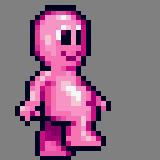
\includegraphics[width=0.11\textwidth]{previews/walk-WALK-03.png}

\includegraphics[width=0.11\textwidth]{previews/walk-WALK-04.png}
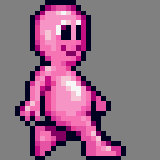
\includegraphics[width=0.11\textwidth]{previews/walk-WALK-05.png}

\includegraphics[width=0.11\textwidth]{previews/walk-WALK-06.png}

\includegraphics[width=0.11\textwidth]{previews/walk-WALK-07.png}
\end{center}

These eight 32$\times$32
\mach{ARGB1555}
bitmap images are an animated
walk cycle.
Because all the images are the same size and format,
they can share the same bitmap handle.
The drawing commands select which image (or \term{cell}) to draw.
For bitmaps drawn with \dcmd{Vertex2ii} the fourth parameter
selects the cell. So for example this code
draws the eight animation frames across the screen:
\eg{examples-cell}
\noindent

\noindent
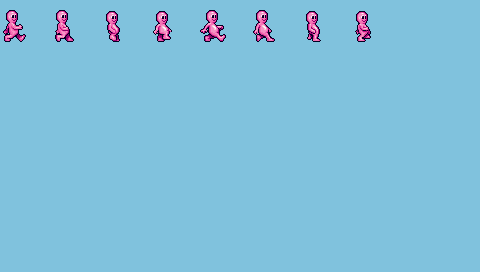
\includegraphics[width=\textwidth,trim=0 216 80 0,clip=true]{assets/0058.png}}

Each bitmap handle can contain up to 128 cells, and the cells are arranged
consecutively in graphics memory.
Cells are useful for animation.
By loading the animation sequence into the cells of a single bitmap handle,
you can animate an object by changing its cell number.

Using the same eight-frame animated sequence,
the \textit{walk} demo animates 256 sprites in a walk cycle crossing the screen.
\index{demos!walk}
Each sprite has a counter that controls its $x$ position and its animation frame.
The color of the sprites changes from black (\mach{0x000000}) at the top of the screen to white (\mach{0xffffff}) at the bottom.

\newpage
\png{walk}
\eg{walk-A}

% \newpage
% \section{Game: Fruit flicker 2000}
% \section{Zoom and shrink}

\newpage
\section{Rotation, zoom and shrink}
\index{rotation}
\index{zoom}
\index{bitmaps!rotating}
\index{bitmaps!zooming}
\png{0043}
\eg{examples-rot1}

Bitmap rotation and zooming is controlled by the
\term{bitmap transform matrix}.
This matrix is part of the graphics state.
It controls the mapping of the bitmap's image pixels onto the screen.
Fortunately, much of the math of the transform matrix is handled by the hardware, so
we can use higher-level operations like rotate and scale.

Here the bitmap is being drawn three times,
with 0$^\circ$, 
22.5$^\circ$,
and finally 45$^\circ$ clockwise rotation,
because \cmd{rotate} operations are cumulative.
Parts of the bitmap disappear as it rotates around its top-left corner.
This version shows what is happening more clearly
because transparency has been turned off using a \dcmd{BlendFunc} of
\mach{(SRC\_ALPHA, ZERO)}:
\png{0044}

\noindent
Each \dcmd{Vertex2ii} draws 128$\times$128 pixels, because that is the size of the bitmap.
However, the source image pixels are determined by the current bitmap transform matrix, and as it
changes the source image rotates.

This rotation is centered on the top-left pixel of the bitmap, pixel $(0, 0)$.
A more useful effect is rotation about the image center,
which in this case is at bitmap pixel $(64, 64)$.
To do this, the steps are:
\begin{enumerate}
\item \textit{translate} the image so that $(64, 64)$ is moved to $(0, 0)$
\item rotate the image around $(0, 0)$ using \cmd{rotate}
\item translate the image back, returning pixel $(0, 0)$ to $(64, 64)$
\end{enumerate}

\noindent
This function \mach{rotate\_64\_64} performs these three steps:

\samepage{
\eg{examples-rota}
}
It uses the \cmd{translate} command to move the bitmap by 64 pixels in both $x$ and $y$.
\cmd{translate} uses 16.16 fixed-point values for its arguments, for subpixel precision,
so here the \mach{F16()} macro does the conversion from integer pixel values.
\png{0045}
\eg{examples-rot3}

\newpage
Scaling the image -- either increasing the scale to zoom it,
or decreasing the scale to shrink it -- uses the \cmd{scale} command.
Here a similar function \mach{scale\_64\_64()} applies a scale around pixel $(64, 64)$.
The first bitmap has no scale.
The second is scaled by a factor of 2.0, doubling it in size.
The third bitmap is scaled by 0.4, shrinking it.

\png{0062}

\eg{examples-scale1}

%%%%%%%%%%%%%%%%%%%%%%%%%%%%%%%%%%%%%%%%%%%%%%%%%%%%%%%%%%%%%%%%%%%%%%%%
\chapter{More on graphics}
\newpage
\section{Lines}
\defidx{LINES}
\index{drawing!lines}
\index{lines}
\label{lines}

\png{lines}

To draw lines, use \mach{Begin(LINES)} or \mach{LINE\_STRIP}.
\mach{LINES} connects every pair of vertices, whereas \mach{LINE\_STRIP} joins all the
vertices together.

\eg{lines-a}

The NightStrike game uses \mach{LINES} to draw spark showers
\index{NightStrike}
that ``pop'' out of each explosion. Each spark is tracked as an
object with a position \mach{(x,y)}, a velocity \mach{(xv,yv)}, and an age.
At the start of the explosion each spark is positioned
at the explosion center, but has a random velocity in \mach{(xv,yv)}.
Every frame the sparks travel along their path, and are drawn by this code:

\eg{nightstrike-sparks}

This draws a line from the spark's current $(x, y)$ position to its \textit{next} position.
The size of the spark (\dcmd{LineWidth}) uses a sinusoidal formula, so that it starts off thin, gets wide, then
becomes thin again at the end of its cycle.
\index{sinusoidal}
\index{explosion}

\begin{center}
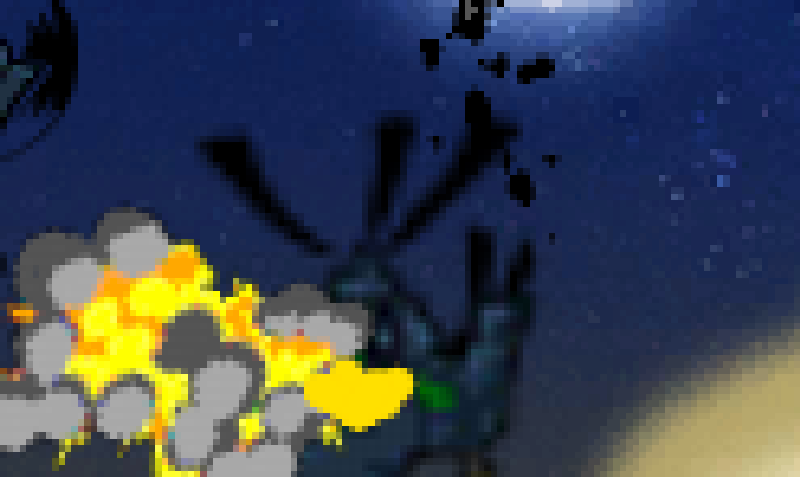
\includegraphics[width=0.3\textwidth]{assets/ns-lines-0000.png}
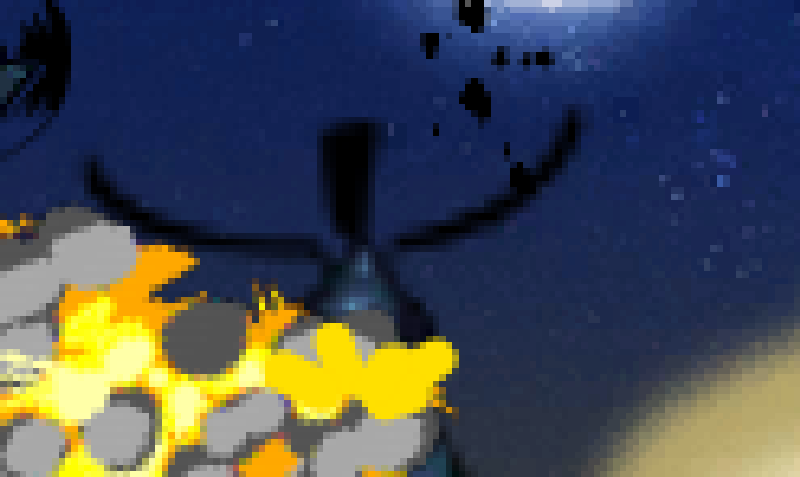
\includegraphics[width=0.3\textwidth]{assets/ns-lines-0001.png}
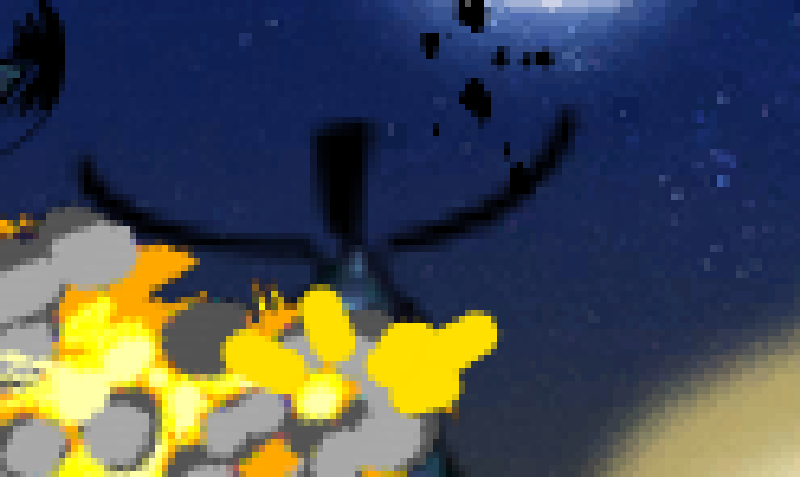
\includegraphics[width=0.3\textwidth]{assets/ns-lines-0002.png}
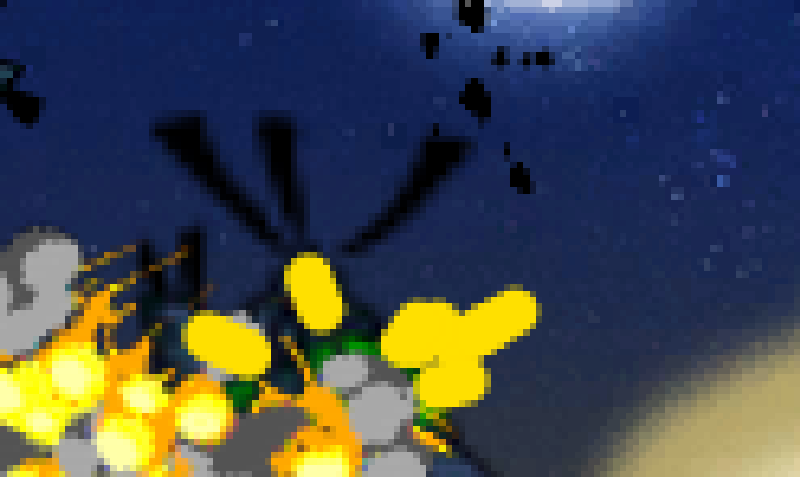
\includegraphics[width=0.3\textwidth]{assets/ns-lines-0003.png}
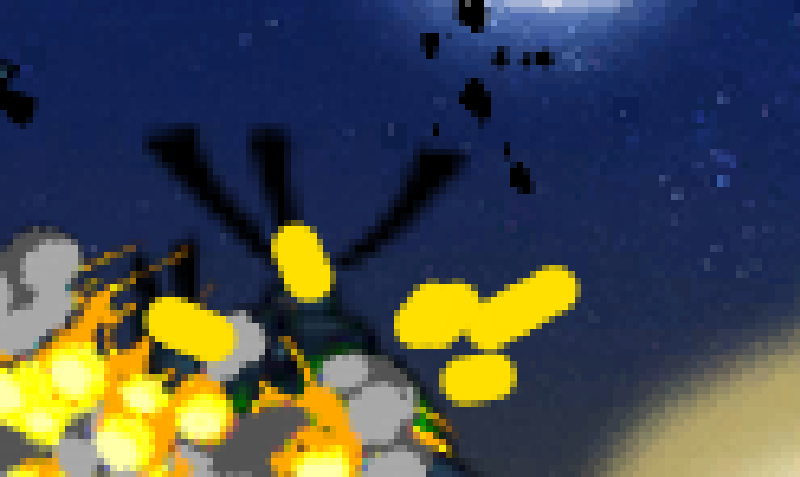
\includegraphics[width=0.3\textwidth]{assets/ns-lines-0004.png}
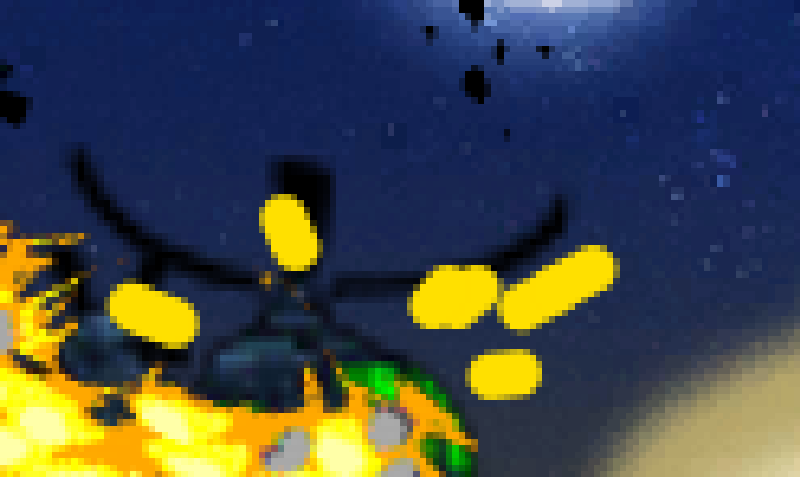
\includegraphics[width=0.3\textwidth]{assets/ns-lines-0005.png}
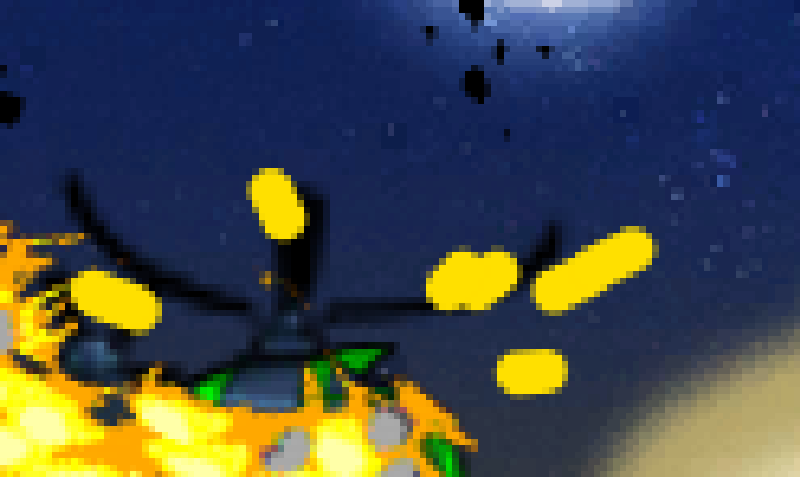
\includegraphics[width=0.3\textwidth]{assets/ns-lines-0006.png}
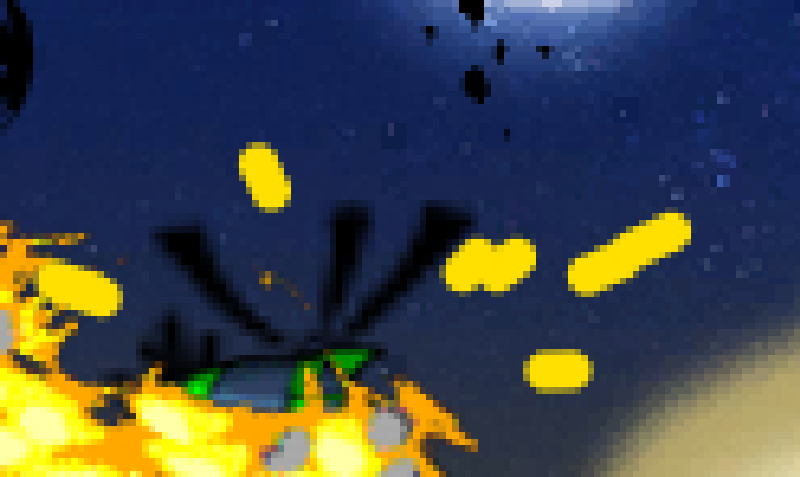
\includegraphics[width=0.3\textwidth]{assets/ns-lines-0007.png}
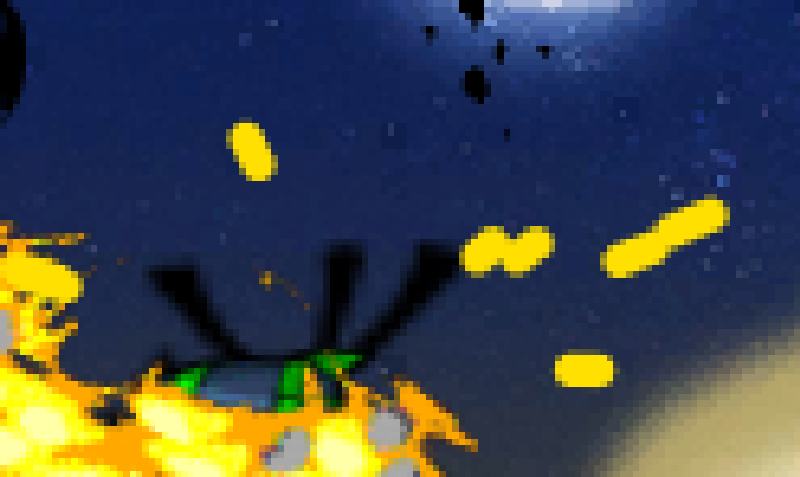
\includegraphics[width=0.3\textwidth]{assets/ns-lines-0008.png}
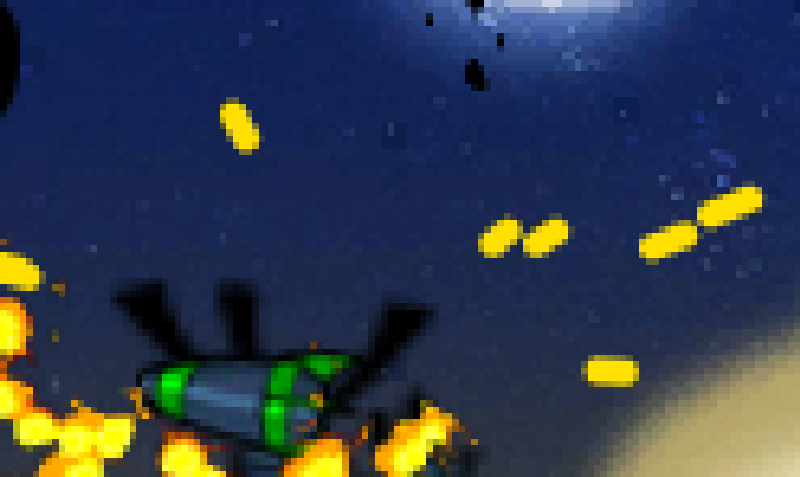
\includegraphics[width=0.3\textwidth]{assets/ns-lines-0009.png}
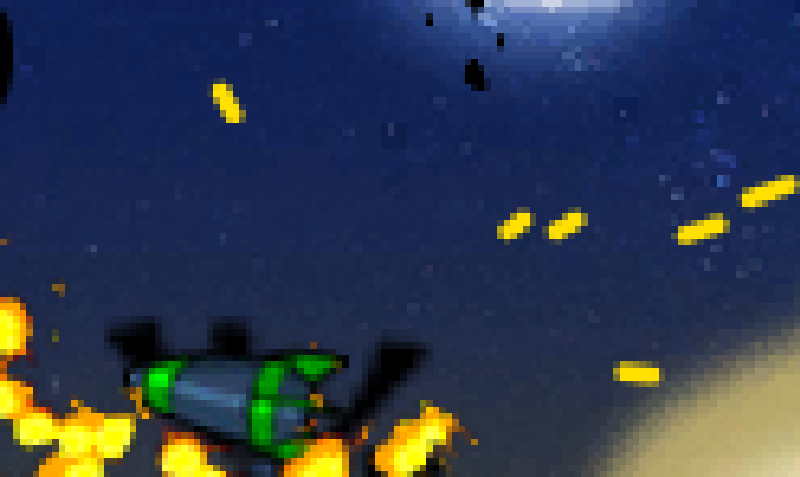
\includegraphics[width=0.3\textwidth]{assets/ns-lines-0010.png}
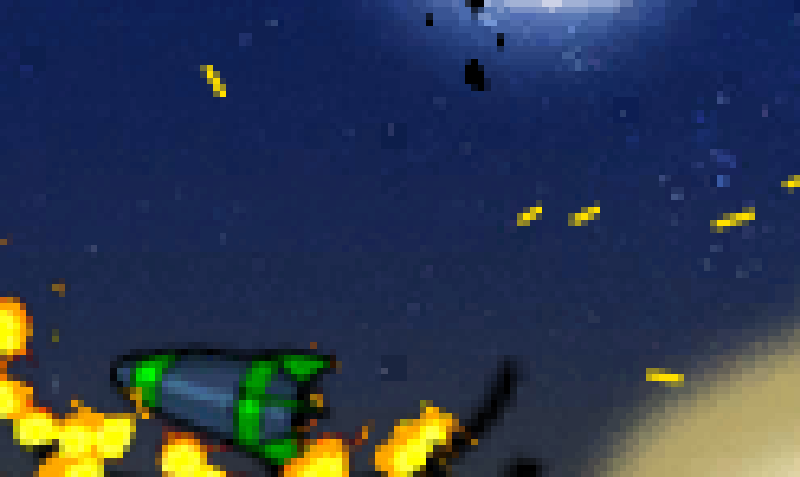
\includegraphics[width=0.3\textwidth]{assets/ns-lines-0011.png}
\end{center}

This 12-frame detail shows the sparks' progress.
The game runs at 60 fps, so the spark sequence 
takes about 1/5th of a second.
\index{sparks}

\newpage
\section{Rectangles}
\defidx{RECTS}
\index{rectangles, drawing}
\index{drawing!rectangles}

\png{0039}

To draw rectangles, use \mach{Begin(RECTS)} and supply opposite corners of the rectangle.
The order of the two corners does not matter.
The rectangles are drawn with round corners,
using the current line width as the corner radius.\index{corner radius}\index{radius, corner}
The round corners are drawn \textit{outside} the rectangle, so increasing the corner radius draws more pixels.
This example draws a 420$\times$20 rectangle three times with increasing corner radius.

\eg{examples-rects}

\section{Gradients}
\label{gradient}
\index{gradient}
\index{drawing!gradients}
\png{0012}
Gradients - smooth color blends across the screen - are a useful graphical element.
You \textit{could} use a large background image of the gradient,
but it's more efficient to use \cmd{gradient}.

\cmd{gradient} draws a smooth gradient on the whole screen, given a starting point and color, and an ending point and color.
In this example the starting point is top-left $(0, 0)$ and the starting color is deep blue (\mach{0x0060c0}).
The ending point is bottom-left $(0, 271)$, deep orange (\mach{0xc06000}).

\eg{examples-grad}

These two points produce a vertical gradient, but \cmd{gradient} can draw gradients at any angle.
You can get a horizontal or diagonal gradient by appropriate placement of the two control points.

\cmd{gradient} used like this writes every pixel on the screen, so it can be used in place of
\dcmd{Clear}.
To draw a gradient on part of the screen, you can use \dcmd{ScissorXY} and \dcmd{ScissorSize} to limit
drawing to a rectangular area. For more complex shapes, \cmd{gradient} can be used with a stencil test.
\clearpage

\section{Blending}
\index{blending}
\png{0040}

\eg{examples-blend1}

Usually each drawn pixel \textit{replaces} the pixel that was on the screen.
This is useful for layering, but sometimes you need a different mixing operation.
\dcmd{BlendFunc} controls this operation.
The first argument to \dcmd{BlendFunc} is the \term{source blend factor}, which controls the incoming
color pixels.
The second is the \term{destination blend factor}, which similarly
controls the pixels that are already in the color buffer.
After the blend factors have modified the colors,
the two results are summed to produce the final pixel color.

\newpage
\begin{center}
\begin{tikzpicture} [scale=0.75]
  \tikzstyle{txt}=[text width=0.15\textwidth,align=center]
  \node [txt]               at (-4.5,4) (pix) {incoming pixel color};
  \node [shape=rect,draw,txt] at (-1.5,4) (sbf) {\textit{source blend factor}};
  \node [txt]               at (1.5,4) (exi) {existing pixel color};
  \node [shape=rect,draw,txt] at (4.5,4) (dbf) {\textit{destination blend factor}};
  \node [shape=circle,draw] at (-3.0,2) (src) {$\times$};
  \node [shape=circle,draw] at (3.0,2) (dst) {$\times$};
  \node [shape=circle,draw] at (0,0) (sum) {+};
  \node [txt]               at (0,-2) (fb) {final pixel color};

  \draw [-latex'] (pix) -- (src);
  \draw [-latex'] (sbf) -- (src);
  \draw [-latex'] (exi) -- (dst);
  \draw [-latex'] (dbf) -- (dst);

  \draw [-latex'] (src) -- (sum);
  \draw [-latex'] (dst) -- (sum);
  \draw [-latex'] (sum) -- (fb);
  % \draw [-latex'] (fb) [out=0,in=120] to (dst);
\end{tikzpicture}
\end{center}

The default mode is
\mach{BlendFunc(SRC\_ALPHA, ONE\_MINUS\_SRC\_ALPHA)}, which means that the incoming pixel color
is mixed with the existing screen color in proportion to the alpha channel value.

Another frequently used mode is
\mach{BlendFunc(SRC\_ALPHA, ONE)}. The \mach{ONE} factor for the destination means that the
incoming pixel color is \textit{added}
to the existing pixel color.
This is useful for glows and overlays.
In the code above you can see this mode means that every disk drawn is added to the existing screen contents,
so their brightness accumulates.

\mach{BlendFunc(SRC\_ALPHA, ZERO)} is the \term{replace} operation; it disables transparency.
The \mach{ZERO} factor for the destination means that existing screen pixels are discarded at the blending stage.

\png{0069}

\newpage
\section{Fonts}
\png{fonts0}

The \gdtwos GPU has sixteen built-in fonts, numbered 16-31.
Numbers 26-31 are the high-quality anti-aliased fonts.
You can also load TrueType (\mach{.ttf}) fonts
using the asset converter (see \xref{assets}).
After loading it, you can use the new font with any of the drawing commands.

\eg{fonts-night}

\begin{center}
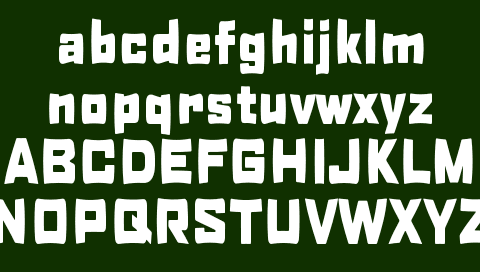
\includegraphics[width=0.7\textwidth]{assets/fonts1.png}
\end{center}

\newpage
\section{Subpixel coordinates}

So far all drawing has used \dcmd{Vertex2ii} to supply the vertices.
\dcmd{Vertex2ii} can only handle $(x,y)$ that are integers in the range 0-511.
What if you want to supply a vertex with a negative coordinate,
or a coordinate that isn't on an exact pixel?
In these cases, you can use \dcmd{Vertex2f}, which uses a finer scale
for $x$ and $y$, and has a much larger range.
\dcmd{Vertex2f} coordinates are in 16ths of a pixel. So this call using
\dcmd{Vertex2ii}:

\begin{framed}
\begin{verbatim}
GD.Vertex2ii(1, 100);
\end{verbatim}
\end{framed}

\noindent
becomes this call using \dcmd{Vertex2f}:

\begin{framed}
\begin{verbatim}
GD.Vertex2f(16, 1600);
\end{verbatim}
\end{framed}

\noindent
but it is often clearer to multiply by 16 explicitly in the code, like this:
\begin{framed}
\begin{verbatim}
GD.Vertex2f(16 * 1, 16 * 100);
\end{verbatim}
\end{framed}

\dcmd{Vertex2f} draws
\mach{POINTS},
\mach{LINES} and
\mach{RECTS}
with much finer precision.
Each of these 16 points is drawn with a $y$ coordinate that increases by 1/16th of a pixel.
As you can see, the graphics system adjusts the shading of the pixels very slightly as the point
moves downwards by 1/16th of a pixel.
This extra precision means that ``pixel'' effects are much less noticable.

\vspace{10pt}
\noindent
\begin{tikzpicture}[scale=0.08928571428571428]
\node[anchor=south west,inner sep=0] (image) at (0,0) {
\includegraphics[width=1.0\textwidth]{assets/subpixel.png}};
\foreach \x in {0,0.1,...,11.3}
  \draw [white] (\x\textwidth,0) -- (\x\textwidth,9.6);
\foreach \y in {0,0.1,...,0.9}
  \draw [white] (0,\y\textwidth) -- (11.2\textwidth,\y\textwidth);
\end{tikzpicture}

\newpage
\section{Angles in Furmans}
\label{furmans}
\index{Furmans}
\index{angles!in Furmans}
\cmdidx{rsin}
\cmdidx{rcos}
\cmdidx{atan2}
\cmdidx{polar}

The GD library refers to angles in several places:

\begin{itemize}
\item the \cmd{rotate} command, which rotates bitmaps, takes an angle parameter
\item the \cmd{dial} command draws a dial widget at a particular angle
\item the widget tracking system, controlled by \cmd{track}, reports the angle of rotary widgets
\item the
\nameref{rsin},
\nameref{rcos},
\nameref{polar} and
\nameref{atan2} math functions all use angles
\end{itemize}

In each case, the angle is specified in Furmans, not in degrees or radians.
A Furman is an angle measure; there are 65536 Furmans in a circle. So

\[
1 \text{ Furman}
\; = \;
\frac{1}{65536} \text{ circle} 
\; = \;
\frac{360}{65536} \text{ degrees}
\; = \;
\frac{2\pi}{65536} \text{radians}
\]

Orientations are represented
by clockwise angles, with an angle of 0 meaning straight down:

\begin{center}
\begin{tikzpicture}[scale=0.75]
    \newcommand{\rb}{3.3}
    \draw (0, 0) circle (\rb);
    \draw (90:\rb) -- (90:4.0) (90:4.4) node {\mach{0x8000}};
    \draw (45:\rb) -- (45:4.0) (45:4.4) node {\mach{0xa000}};
    \draw (0:\rb) -- (0:4.0) (0:5.0) node {\mach{0xc000}};
    \draw (315:\rb) -- (315:4.0) (315:4.4) node {\mach{0xe000}};
    \draw (270:\rb) -- (270:4.0) (270:4.4) node {\mach{0}};
    \draw (225:\rb) -- (225:4.0) (225:4.4) node {\mach{0x2000}};
    \draw (180:\rb) -- (180:4.0) (180:5.0) node {\mach{0x4000}};
    \draw (135:\rb) -- (135:4.0) (135:4.4) node {\mach{0x6000}};

    % \draw (45:3.9) -- (45:4.8)     [<-, thick] node [right] {\reg{CMD\_READ}};
    % \draw (-200:3.9) -- (-200:4.8) [<-, thick] node [left] {\reg{CMD\_WRITE}};

\end{tikzpicture}
\end{center}
As a convenience, the GD library defines a macro \mach{DEGREES()}, which converts angles in degrees to Furmans:
\begin{verbatim}
#define DEGREES(n) ((65536UL * (n)) / 360)
\end{verbatim}

\newpage
The advantage of representing angles as Furmans is that they make angular arithmetic significantly cheaper.
For example, when incrementing angles for a rotating object, normal
16-bit arithmetic means that the Furman measurement wraps from 65535
back to zero.

\begin{center}
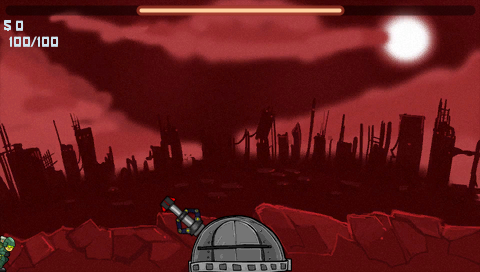
\includegraphics[width=0.7\textwidth]{assets/angle.png}
\end{center}

\index{tracking controls}
In the NightStrike game
\index{NightStrike}
the player's touch controls the angle of the gun turret.
At startup, the game requests the GPU track angles for any touch on tag number
\mach{0x01}:
\eg{nightstrike-cmd_track}
\noindent
After the \cmd{track} command,
\mach{GD.inputs.track\_val}
holds the angle in Furmans from screen position (240, 271) to the touch location.
The game copies this value into the turret's angle variable.
\eg{nightstrike-track}
When the turret is drawn, the angle variable is used with \cmd{rotate} to rotate the turret's bitmap,
\cmdidx{cmd\_rotate}
which is in the ``0 Furmans'' orientation:
\begin{center}

\includegraphics[width=0.10\textwidth]{assets/turret.png}
\end{center}

\newpage
\section{The context stack}
\index{context}
\png{context}

\eg{nightstrike-context}

The function \mach{blocktext}, used in \textit{NightStrike}'s title screen,
\index{NightStrike}
draws the string \mach{s} with a black outline around the text.
To do this, it changes the color to black using \dcmd{ColorRGB}, and draws the text four times slightly offset.
Now it needs to draw the text itself, in the original color.
But the original color is lost, because it was changed to black.

The \dcmd{SaveContext} preserves all the graphics state -- including the color -- in a private storage area.
When \dcmd{RestoreContext} executes, it copies this saved state back.
Hence the color is restored to the value it had at the original \dcmd{SaveContext}.

Using \dcmd{SaveContext} or \dcmd{RestoreContext}, functions can change graphics state,
and then restore it afterwards.
As far as any caller is concerned, the function leaves the state untouched.
The GPU has enough internal storage to preserve three extra copies of the graphics state in this way.


% \section{Color, tag and stencil}
% \section{Clock}
% \section{Widgets}

%%%%%%%%%%%%%%%%%%%%%%%%%%%%%%%%%%%%%%%%%%%%%%%%%%%%%%%%%%%%%%%%%%%%%%%%
\chapter{Touch}

\section{Reading the touch inputs}

The function \nameref{getinputs} reads all the Gameduino 2's inputs, including the touch sensors.
After making this call, you can read the touch coordinates from
\mach{GD.inputs.x} and
\mach{GD.inputs.y}.
The best time in the game cycle to sense inputs is just before starting to draw the screen,
so a frequent pattern is:
\eg{simon-touch}

If there is no touch, then both \mach{GD.inputs.x} and \mach{GD.inputs.y} are set to -32768.
The touch $(x,y)$ are \term{screen pixel coordinates}, so they range $(0 \le x \le 479)$ and $(0 \le y \le 271)$.
To convert these pixel coordinates into subpixel coordinates, multiply by 16.  For example:
\eg{blobs-xy}

\newpage
\section{Demo: blobs}
\index{demos!blobs}
\png{blobs}
The ``blobs'' demo lets you sketch a trail of groovy expanding colored circles with a finger or stylus.
The code keeps track of 128 points, animating each with radius and alpha to create a pleasing
``fade out'' effect.

At startup, \mach{begin()} sets all the blobs' positions to off screen.

\eg{blobs-a}

If the screen is being touched, the subpixel coordinates of the touch are added into the \mach{blobs} ring.
Each blob's transparency and radius depends on its age.
The ``random'' color is actually computed using modulo arithmetic.

\eg{blobs-b}

\section{Tags}

Tagging is a GPU feature that makes touch detection easier.
In many situations the exact coordinates of the touch are not important -- you are only interested in \textit{what} has been touched.
As you draw each object on the screen, you can tag its pixels with a byte value.
For example, to create a 'OK' button, you can tag its pixels with code 44.
Then each time the user touches the button, the number 44 appears in the tag register.
Tag values are a single byte, ranging from
0 to 255.
However, the hardware uses a tag value of 255 to indicate ``no touch", so the usable range of values is 0 to 254.

\png{0005}

This example sets the \dcmd{Tag} value before drawing each number. % using \cmd{number}.
Because the pixels belonging to each number are then ``tagged'', \mach{GD.inputs.tag} is set to the number being currently touched,
and the Arduino can access it and print it on the serial output.

\eg{examples-h}

\newpage
\section{Sketching}
\label{sketching}
\index{sketching}
\cmdidx{cmd\_sketch}

\png{sketching}

Sketching here means taking touch input and plotting pixels.
The \gdtwo GPU has built-in sketching  so you can `paint'
pixels into the bitmap without any input from the Arduino.
The \cmd{sketch} command starts sketching.
When you want sketching to stop, call \cmd{stop}.
Note the call to \mach{GD.flush()}.
This forces any buffered commands to the GPU immediately.

\eg{sketch-a}

\newpage
\section{Widgets and tracking controls}
\label{widgets}
\index{widgets}
\index{tracking controls}
\index{user interface}

\png{widgets3d}

\gdtwo has a rich set of widgets: dials, buttons, gauges, sliders and scroll bars.
To help manage the user interactions with the adjustable widgets, a feature called \textit{tracking controls}
extends the simple tag system.
Using tags, the program can know when an object is touched.
With a tracking control, the program can also know the relative position of the touch.

\index{demos!widgets}
The \mach{widgets} demo draws all widget types, and
for the three adjustable widgets -- the dial, slider and toggle -- uses tracking controls to manage their touches.
Each adjustable widget is drawn with a unique tag value, here
\mach{200},
\mach{201} and
\mach{202}.

\vspace{10pt}

\begin{tikzpicture}
  \node[anchor=south west,inner sep=0,opacity=0.2] (image) at (0,0) {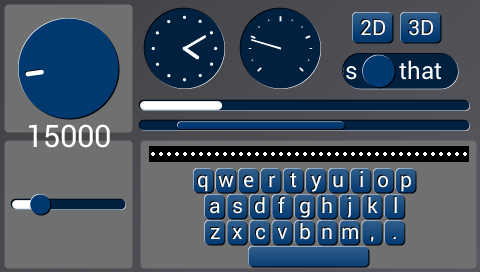
\includegraphics[width=0.9\textwidth]{assets/widgets3d.png}};
  \begin{scope}[x={(image.south east)},y={(image.north west)},xscale=0.20833333333333334,yshift=0.51\textwidth,yscale=-0.3676470588235294]

    \draw[black, thick] (0.68,0.68) circle (0.50);
    \node at (0.68,0.68) {200};

    % \draw[black, ultra thick] (0.16,1.99) rectangle (0.40);
    % \node at (0.16,1.99) {201};

    \node [draw,
      shape=rounded rectangle,
          minimum width=28mm,
          minimum height=0mm,
          ]
        at (0.68,2.04) {201};

    \node [draw,
      shape=rounded rectangle,
          minimum width=28mm,
          minimum height=8mm,
          ]
        at (4.00,0.69) {202};

  \end{scope}
\end{tikzpicture}

\newpage
The program then tells the GPU to track touches on the three regions. First it draws the dial with tag 200.
Then it calls \cmd{track} so that the GPU will track touches for that particular tag, and compute the position
relative to pixel position (68, 68), the center of the dial:
\eg{widgets-dial}
\index{angles!rotary tracking}

Similarly for the linear widgets, the slider and toggle:
\eg{widgets-linear}

With these set up, the program can detect a relative touch on any widget by reading
\mach{GD.inputs.track\_tag} and
\mach{GD.inputs.track\_val}.
The value in \mach{GD.inputs.track\_val} is an unsigned 16-bit number in the range 0-65535.
For the rotary track -- the dial -- this is the touch angle in Furmans.
For the linear tracks, it is the touch position within the rectangle.
0 means far left and 65535 means far right.
\eg{widgets-track}

%%%%%%%%%%%%%%%%%%%%%%%%%%%%%%%%%%%%%%%%%%%%%%%%%%%%%%%%%%%%%%%%%%%%%%%%
\chapter{Sound}

Gameduino 2 has two sound systems.
The first -- the \term{synthesizer} -- can generate a set of fixed sounds and musical notes.
The synthesizer is useful for quickly adding audio to a project, but because the sound set is fixed, is not very flexible.
The second is the \term{sample playback}.
It plays sampled audio from main memory in a variety of formats.
This system is much more flexible but you will need to prepare and load samples into RAM.

\section{Clicks and pops}

The synthesizer provides several short ``percussive'' sounds, mostly for use in user interfaces.
To trigger the sound, call \mach{GD.play()} with the sound ID.
The full list of available sounds is:

\vspace{10pt}
\begin{tabular}{l}
\mach{CLICK} \\
\mach{SWITCH} \\
\mach{COWBELL} \\
\mach{NOTCH} \\
\mach{HIHAT} \\
\mach{KICKDRUM} \\
\mach{POP} \\
\mach{CLACK} \\
\mach{CHACK} \\
\end{tabular}
\vspace{10pt}

\section{Instrument playback}

The synthesizer can also produce musical instrument notes.
Again, calling \mach{GD.play()} triggers the sound, and the first parameter
is an instrument:

\index{instruments}
\label{instruments}

\vspace{10pt}
\begin{tabular}{l}
\mach{HARP} \\
\mach{XYLOPHONE} \\
\mach{TUBA} \\
\mach{GLOCKENSPIEL} \\
\mach{ORGAN} \\
\mach{TRUMPET} \\
\mach{PIANO} \\
\mach{CHIMES} \\
\mach{MUSICBOX} \\
\mach{BELL}
\end{tabular}
\vspace{10pt}

\noindent
In this case \mach{GD.play()} also accepts an optional second argument that specifies a MIDI note number 
in the range 21 to 108. If this argument is omitted then it plays in C4, MIDI note 60.

The synthesizer can also play a few other miscellaneous sounds.
Instruments
\mach{SQUAREWAVE},
\mach{SINEWAVE},
\mach{SAWTOOTH} and
\mach{TRIANGLE}
generate continuous simple waves, useful for retro effects.
Instruments
\mach{BEEPING},
\mach{ALARM},
\mach{WARBLE} and
\mach{CAROUSEL}
generate various alarm tones.
And the ASCII codes '0' - '9', '*' and '\#' generate the corresponding touch-tone DTMF tones.

To detect when a note has finished playing, read the hardware's \mach{PLAY} register.
When it is zero, the note is finished:
\eg{examples-waitnote}

\tablefirsthead{%
MIDI note & ANSI note & freq. (Hz) \\
\hline
}
\tablehead{%
MIDI note & ANSI note & freq. (Hz) \\
\hline
}
\footnotesize
\twocolumn
\begin{spacing}{0.99}
\begin{supertabular}{ccc}
\index{MIDI notes|boldindex}
\label{MIDI}
21  & A0  &  27.5 \\
22  & A$^\#$0 &  29.1 \\
23  & B0  &  30.9 \\
24  & C1  &  32.7 \\
25  & C\#1 &  34.6 \\
26  & D1  &  36.7 \\
27  & D\#1 &  38.9 \\
28  & E1  &  41.2 \\
29  & F1  &  43.7 \\
30  & F\#1 &  46.2 \\
31  & G1  &  49.0 \\
32  & G\#1 &  51.9  \\
33  & A1  &  55.0  \\
34  & A\#1 &  58.3  \\
35  & B1  &  61.7  \\
36  & C2  &  65.4  \\
37  & C\#2 &  69.3  \\
38  & D2  &  73.4  \\
39  & D\#2 &  77.8  \\
40  & E2  &  82.4  \\
41  & F2  &  87.3  \\
42  & F\#2 &  92.5  \\
43  & G2  &  98.0  \\
44  & G\#2 & 103.8  \\
45  & A2  & 110.0  \\
46  & A\#2 & 116.5  \\
47  & B2  & 123.5  \\
48  & C3  & 130.8  \\
49  & C\#3 & 138.6  \\
50  & D3  & 146.8  \\
51  & D\#3 & 155.6  \\
52  & E3  & 164.8  \\
53  & F3  & 174.6  \\
54  & F\#3 & 185.0  \\
55  & G3  & 196.0  \\
56  & G\#3 & 207.7  \\
57  & A3  & 220.0  \\
58  & A\#3 & 233.1  \\
59  & B3  & 246.9  \\
60  & C4  & 261.6  \\
61  & C\#4 & 277.2  \\
62  & D4  & 293.7  \\
63  & D\#4 & 311.1  \\
64  & E4  & 329.6  \\
65  & F4  & 349.2  \\
66  & F\#4 & 370.0  \\
67  & G4  & 392.0  \\
68  & G\#4 & 415.3  \\
69  & A4  & 440.0  \\
70  & A\#4 & 466.2  \\
71  & B4  & 493.9  \\
72  & C5  & 523.3  \\
73  & C\#5 & 554.4  \\
74  & D5  & 587.3  \\
75  & D\#5 & 622.3  \\
76  & E5  & 659.3  \\
77  & F5  & 698.5  \\
78  & F\#5 & 740.0  \\
79  & G5  & 784.0  \\
80  & G\#5 & 830.6  \\
81  & A5  & 880.0  \\
82  & A\#5 & 932.3  \\
83  & B5  & 987.8  \\
84  & C6  & 1046.5 \\
85  & C\#6 & 1108.7 \\
86  & D6  & 1174.7 \\
87  & D\#6 & 1244.5 \\
88  & E6  & 1318.5 \\
89  & F6  & 1396.9 \\
90  & F\#6 & 1480.0 \\
91  & G6  & 1568.0 \\
92  & G\#6 & 1661.2 \\
93  & A6  & 1760.0 \\
94  & A\#6 & 1864.7 \\
95  & B6  & 1975.5 \\
96  & C7  & 2093.0 \\
97  & C\#7 & 2217.5 \\
98  & D7  & 2349.3 \\
99  & D\#7 & 2489.0 \\
100 & E7  & 2637.0 \\
101 & F7  & 2793.8 \\
102 & F\#7 & 2960.0 \\
103 & G7  & 3136.0 \\
104 & G\#7 & 3322.4 \\
105 & A7  & 3520.0 \\
106 & A\#7 & 3729.3 \\
107 & B7  & 3951.1 \\
108 & C8  & 4186.0 \\
\end{supertabular}
\end{spacing}
\onecolumn
\normalsize

\section{Samples}
\index{samples}

\gdtwos audio system can also play back samples.
The sample playback system is independent -- you can play a sample while playing a fixed sound, and the
hardware will mix the two sounds together, according to their assigned volumes.

To play back a sample from memory, call \mach{GD.sample} with the
sample's base address, length, frequency and format as arguments.
So if you have a ULAW sample at address 0, of length 22050 bytes,
with frequency 44100 Hz, you play it by calling:

\begin{framed}
\begin{verbatim}
GD.sample(0, 22050, 44100, ULAW_SAMPLES);
\end{verbatim}
\end{framed}

Three sample formats are supported:

\vspace{10pt}
\begin{tabular}{ccl}
format & bit per sample & encoding \\
\hline \\
\mach{LINEAR\_SAMPLES} & 8 & signed 8-bit linear, -128 to 127 \\
\mach{ULAW\_SAMPLES} & 8 & standard 8-bit encoded $\mu$-law \\
\mach{ADPCM\_SAMPLES} & 4 & standard IMA ADPCM \\
\end{tabular}
\vspace{10pt}

\gdtwos asset converter tool (see \xref{assets}) converts mono \mach{.wav}
files to any of these formats.
The hardware supports playback rates up to 48 kHz, and at this rate
the sound quality of ADPCM samples is similar to AM radio.
Of course this rate uses 24 kBytes/s of memory.
To save memory, use ADPCM with a low sample rate. The \mach{noisy} demo
plays back voice samples of the digits 0-9, encoded in ADPCM at 8 kHz.
The samples are quite intelligible, and together take about 26 kBytes of
graphics memory.

Note that there is a hardware-imposed restriction on the arguments to \mach{GD.sample()}.
The base address and length must be multiples of 8.
However, the asset converter tool aligns and pads samples automatically,
so that you don't need to do anything special.

\newpage
\eg{noisy-A}

\newpage
\section{Continuous playback}

\png{song}

For long samples, keeping the entire sample in graphics memory is usually not practical.
Instead the hardware's sample playback system can continuously play back a loop of samples, while the Arduino keeps the loop fed with
fresh samples from SDcard.
The \mach{Streamer} class in the GD2 library conveniently handles these details.
To use it, call its \mach{begin()} method with the name of a music file on the microSD card.
\mach{Streamer} defaults to a sample rate of 44.1 kHz, and IMA ADPCM sample encoding.
It uses a 4K buffer for the streaming samples, located at the very top of graphics memory.

Calling \mach{Streamer}'s \mach{feed()} method reads samples from the file into the buffer.
Your application should call \mach{feed()} often enough to prevent the buffer running out of samples.
Here the code calls \mach{stream.feed()} once per frame.

\mach{Streamer} can also tell how far the file has progressed.
\mach{progress()} returns a pair of 16-bit numbers,
\mach{val} and \mach{range}, which represent progress as a fraction $(\mach{val} / \mach{range})$.
This example passes \mach{val} and \mach{range} directly to a \cmd{slider} widget.

If you have the \mach{sox} audio utility installed, you can convert \mach{.wav} samples to ADPCM IMA format on the command-line like this:

\begin{framed}
\begin{verbatim}
$ sox mesmeriz.wav -c 1 mesmeriz.ima
$ play -r 44100 mesmeriz.ima
\end{verbatim}
\end{framed}

The \mach{play} plays back the converted file.
Because \mach{.ima} is a headerless format, \mach{play} needs to know the sample rate, in this case 44100 Hz.

\eg{song-A}

%%%%%%%%%%%%%%%%%%%%%%%%%%%%%%%%%%%%%%%%%%%%%%%%%%%%%%%%%%%%%%%%%%%%%%%%
\chapter{Accelerometer}

\begin{center}
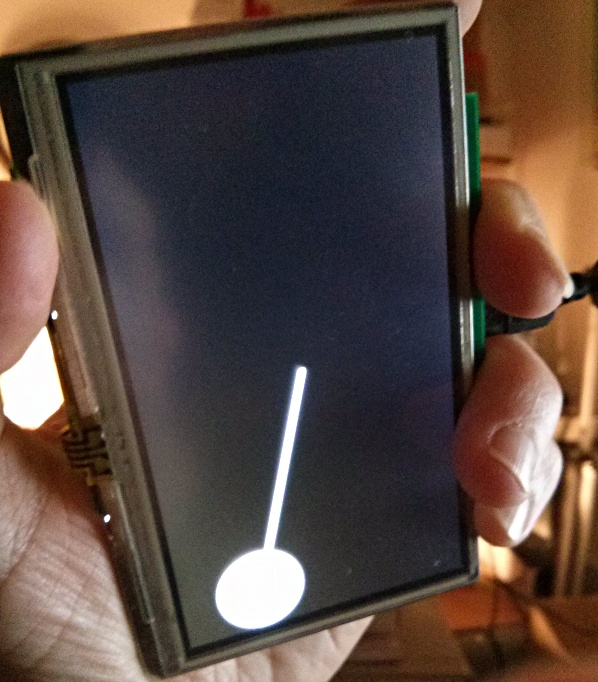
\includegraphics[width=0.4\textwidth]{assets/accel.jpg}
\end{center}

\gdtwo has a 3-axis accelerometer sensor connected to the Arduino's analog inputs A0, A1 and A2.
To read the accelerometer inputs, call \dcmd{getaccel} like this:

\begin{framed}
\begin{verbatim}
int x, y, z;
GD.get_accel(x, y, z);
\end{verbatim}
\end{framed}

\noindent
\mach{get\_accel()} corrects the values so that the force of gravity, 1G, gives a deflection in
\mach{x},
\mach{y} or
\mach{z} of 256.
Tilting \gdtwo all the way to the left, for example, gives
\mach{x} = -256,
\mach{y} = 0,
\mach{z} =0.
Because the accelerometer is an analog input, these values are only approximate,
and in the \mach{tilt} demo you can see that there is a little ``noise'' in the accelerometer reports.

\eg{tilt-A}

%%%%%%%%%%%%%%%%%%%%%%%%%%%%%%%%%%%%%%%%%%%%%%%%%%%%%%%%%%%%%%%%%%%%%%%%
\chapter{MicroSD card}

\gdtwo includes a standard microSD card slot.
It is connected to the same SPI bus as \gdtwos GPU,
and is enabled by Arduino pin 9.
There are several software libraries available for driving microSD cards.
The GD library includes a lightweight library that handles FAT microSD cards,
and integrates with the GD graphics system.

MicroSD files are usually fed directly to the GPU's command stream.
The \mach{GD.load()} command does exactly this: it reads a file from the microSD card
and copies its contents to the \gdtwo's GPU.
For example, to load a JPEG file, executing:

\begin{framed}
\begin{verbatim}
GD.cmd_loadimage(0);
GD.load("kitten.jpg");
\end{verbatim}
\end{framed}

\noindent
The \cmd{loadimage} tells the GPU to expect a JPEG, and then \nameref{load} streams all the JPEG data into the GPU.
As another example, loading 16 Kbytes of raw data from ``\mach{mem.raw}" from the microSD card can be done with:

\begin{framed}
\begin{verbatim}
GD.cmd_memwrite(0, 16384);
GD.load("mem.raw");
\end{verbatim}
\end{framed}

\noindent
Again, \cmd{memwrite} tells the GPU to expect the following data, and then \nameref{load} streams the data in.

The files with suffix \mach{.gd2} created by the asset converter (\xref{assets}) are pure command streams,
just by executing:

\begin{framed}
\begin{verbatim}
GD.load("frogger.gd2");
\end{verbatim}
\end{framed}

\noindent
all the graphics required by the \mach{frogger} game are loaded into memory, and all bitmap handles are set up.
When the asset converter generates the header file \mach{frogger\_assets.h}, it includes a line:

\begin{framed}
\begin{verbatim}
#define LOAD_ASSETS()   GD.load("frogger.gd2")
\end{verbatim}
\end{framed}

\noindent
So the \mach{frogger} sketch can just use \mach{LOAD\_ASSETS()} in its \mach{setup()} to set up all its graphics resources.

% \section{Reading files}
% \section{Reading directories}


\part{Reference}

%%%%%%%%%%%%%%%%%%%%%%%%%%%%%%%%%%%%%%%%%%%%%%%%%%%%%%%%%%%%%%%%%%%%%%%%
\chapter{Drawing commands}

\newcommand{\drawcmd}[2]{
\newpage
\section{\texttt{#1}}
\label{#1}
\index{#1@\mach{#1()}|boldindex}

#2

}

\newcommand{\lightcmd}[3]{
\section{\texttt{#1}}
\label{#2}
\index{#1@\mach{#1()}|boldindex}


}

\drawcmd{AlphaFunc}{Sets the alpha-test function}

\begin{framed}
\begin{verbatim}
void AlphaFunc(byte func,
               byte ref);
\end{verbatim}
\end{framed}

\begin{tabular}{lp{0.8 \textwidth}}

\\ \mach{func} & comparison function, one of
        \mach{NEVER}, \mach{LESS}, \mach{LEQUAL}, \mach{GREATER}, \mach{GEQUAL}, \mach{EQUAL}, \mach{NOTEQUAL}, or \mach{ALWAYS} \\

\\ \mach{ref} & reference value for comparison function \\

\end{tabular}

\vspace{10pt}
The alpha test function tests each pixel's
alpha value, and only draws the pixel
if the test passes.
For example
\begin{verbatim}
  GD.AlphaText(GEQUAL, 160);
\end{verbatim}
means that only pixels with $(A \ge 160)$ are drawn.  
The default state is \mach{ALWAYS}, which means that pixels are always drawn.
\minipng{0032}
\eg{examples-alphafunc}

\drawcmd{Begin}{Selects the graphics primitive for drawing}

\begin{framed}
\begin{verbatim}
void Begin(byte prim);
\end{verbatim}
\end{framed}

\begin{tabular}{lp{0.8 \textwidth}}

\\ \mach{prim} & one of
\mach{BITMAPS},
\mach{POINTS},
\mach{LINES},
\mach{LINE\_STRIP},
\mach{EDGE\_STRIP\_R},
\mach{EDGE\_STRIP\_L},
\mach{EDGE\_STRIP\_A},
\mach{EDGE\_STRIP\_B} or
\mach{RECTS} \\
\end{tabular}

\vspace{10pt}
The \mach{Begin} command sets the current graphics draw primitve.
It does not draw anything - that is done by a later \nameref{Vertex2f} or \nameref{Vertex2ii} command.
The drawing primitive can be:

\vspace{10pt}

\begin{tabular}{lp{0.8 \textwidth}}
\mach{BITMAPS     } & each vertex draws a bitmap \\
\mach{POINTS      } & each vertex draws an anti-aliased point  \\
\mach{LINES       } & each pair of vertices draws an anti-aliased line \\
\mach{RECTS       } & each pair of vertices draws an anti-aliased rectangle \\
\mach{LINE\_STRIP  } & the vertices define a connected line segment \\
\mach{EDGE\_STRIP\_A} & like \mach{LINE\_STRIP}, but draws pixels above the line \\
\mach{EDGE\_STRIP\_B} & like \mach{LINE\_STRIP}, but draws pixels below the line \\
\mach{EDGE\_STRIP\_L} & like \mach{LINE\_STRIP}, but draws pixels left of the line \\
\mach{EDGE\_STRIP\_R} & like \mach{LINE\_STRIP}, but draws pixels right of the line
\end{tabular}

\png{0047}

\drawcmd{BitmapHandle}{Sets the bitmap handle}

\begin{framed}
\begin{verbatim}
void BitmapHandle(byte handle);
\end{verbatim}
\end{framed}

\begin{tabular}{lp{0.8 \textwidth}}

\\ \mach{handle} & integer handle number, 0-15 \\

\end{tabular}

\vspace{10pt}
The \mach{BitmapHandle} command sets the current bitmap handle, used by
\nameref{Vertex2f},
\nameref{BitmapSource},
\nameref{BitmapLayout} and
\nameref{BitmapSize}.

The bitmap handle is part of the graphics context; its default value is 0.



\drawcmd{BitmapLayout}{Sets the bitmap layout}

\begin{framed}
\begin{verbatim}
void BitmapLayout(byte format,
                  uint16_t linestride,
                  uint16_t height);
\end{verbatim}
\end{framed}

\begin{tabular}{lp{0.8 \textwidth}}

\\ \mach{format} & pixel format of the bitmap, one of:
\mach{ARGB1555},
\mach{L1},
\mach{L4},
\mach{L8},
\mach{RGB332},
\mach{ARGB2},
\mach{ARGB4},
\mach{RGB565},
\mach{PALETTED},
\mach{TEXT8X8},
\mach{TEXTVGA},
\mach{BARGRAPH}.
\\

\\ \mach{linestride} & the size in bytes of one line of the bitmap in memory \\

\\ \mach{height} & height of the bitmap in pixels \\

\end{tabular}

\vspace{10pt}
The \mach{BitmapLayout} command sets the current bitmap's layout in memory.
The \mach{format} controls how memory data is converted into pixels. 
Each pixel in memory is 1,4,8 or 16 bits. The color is extracted from these bits as follows,
where ``v'' is the pixel data.

\vspace{10pt}
\begin{tabular}{cccccc}
format           & bits per & alpha        & red   & green & blue \\
                 &  pixel   &              &       &       &      \\
\hline
\mach{L1}        &    1     & v$_0$        &  1.0  &  1.0  &  1.0 \\
\mach{L4}        &    4     & v$_{3..0}$   &  1.0  &  1.0  &  1.0 \\
\mach{L8}        &    8     & v$_{7..0}$   &  1.0  &  1.0  &  1.0 \\
\hline
\mach{RGB332}    &    8     & 1.0          &  v$_{7..5}$   &  v$_{4..2}$  &  v$_{1..0}$ \\
\mach{RGB565}    &    16    & 1.0          &  v$_{15..1}$  &  v$_{10..5}$ &  v$_{4..0}$ \\
\hline
\mach{ARGB2}     &    8     & v$_{7..6}$   &  v$_{5..4}$   &  v$_{3..2}$  &  v$_{1..0}$ \\
\mach{ARGB4}     &    16    & v$_{15..12}$ &  v$_{11..8}$  &  v$_{7..4}$  &  v$_{3..0}$ \\
\end{tabular}
\vspace{10pt}

1 and 4 bit pixels are packed in bytes from left to right, so
leftmost pixels in the bitmap occupy the most significant bits in a byte.
16 bit pixels are little-endian in graphics memory, and must be aligned on even memory boundaries.

\mach{PALETTED} format uses 8 bits per pixel, each pixel is an index
into the 256 entry 32-bit color table loaded at \mach{RAM\_PALETTE}.
% \mach{TEXT8X8} interpret each byte in the bitmap as an index into a character array, with a character size of 8x8 pixels.
% \mach{TEXTVGA} interprets memory in the same format as an IBM PC VGA graphic controller, 8 bits of character attribute and an 8-bit character code. The character size is 8x16.


\drawcmd{BitmapSize}{Sets the bitmap size and appearance}

\begin{framed}
\begin{verbatim}
void BitmapSize(byte filter,
                byte wrapx,
                byte wrapy,
                uint16_t width,
                uint16_t height);
\end{verbatim}
\end{framed}

\begin{tabular}{lp{0.8 \textwidth}}

\\ \mach{filter} & bitmap pixel filtering, \mach{NEAREST} or \mach{BILINEAR} \\

\\ \mach{wrapx} & $x$ wrapping mode, \mach{BORDER} or \mach{REPEAT} \\

\\ \mach{wrapy} & $y$ wrapping mode, \mach{BORDER} or \mach{REPEAT} \\

\\ \mach{width} & on-screen drawn width, in pixels \\

\\ \mach{height} & on-screen drawn height, in pixels \\

\end{tabular}

\vspace{10pt}
The \mach{BitmapSize} command controls how the current bitmap appears on screen.



\drawcmd{BitmapSource}{Sets the bitmap source address}

\begin{framed}
\begin{verbatim}
void BitmapSource(uint32_t addr);
\end{verbatim}
\end{framed}

\begin{tabular}{lp{0.8 \textwidth}}

\\ \mach{addr} & base address for bitmap \mach{0x00000} - \mach{0x3ffff} \\

\end{tabular}

\vspace{10pt}
The \mach{BitmapSource} command sets the base address for the bitmap.
For 16-bit bitmaps, this address must be even.



\drawcmd{BlendFunc}{Sets the color blend function}

\begin{framed}
\begin{verbatim}
void BlendFunc(byte src,
               byte dst);
\end{verbatim}
\end{framed}

\begin{tabular}{lp{0.8 \textwidth}}

\\ \mach{src} & source blend factor, one of
\mach{ZERO},
\mach{ONE},
\mach{SRC\_ALPHA},
\mach{DST\_ALPHA},
\mach{ONE\_MINUS\_SRC\_ALPHA},
\mach{ONE\_MINUS\_DST\_ALPHA}.  \\

\\ \mach{dst} & destination blend factor, one of
\mach{ZERO},
\mach{ONE},
\mach{SRC\_ALPHA},
\mach{DST\_ALPHA},
\mach{ONE\_MINUS\_SRC\_ALPHA},
\mach{ONE\_MINUS\_DST\_ALPHA}.  \\

\end{tabular}

\vspace{10pt}
The \mach{BlendFunc} command sets the blend function used to combine pixels
with the contents of the frame buffer.
Each incoming pixel's color is multiplied by the source blend factor, and each frame buffer pixel
is multiplied by the destination blend factor.
These two results are added to give the final pixel color.

\minipng{0031}
\eg{examples-blendfunc}


% \drawcmd{Call}{Something}
% 
% \begin{framed}
% \begin{verbatim}
% void Call(uint16_t dest);
% \end{verbatim}
% \end{framed}
% 
% \begin{tabular}{lp{0.8 \textwidth}}
% 
% \\ \mach{dest} & something \\
% 
% \end{tabular}
% 
% \vspace{10pt}
% The \mach{Call} command

\drawcmd{Cell}{Sets the bitmap cell}

\begin{framed}
\begin{verbatim}
void Cell(byte cell);
\end{verbatim}
\end{framed}

\begin{tabular}{lp{0.8 \textwidth}}

\\ \mach{cell} & cell number 0-127 \\

\end{tabular}

\vspace{10pt}
The \mach{Cell} command sets the current bitmap cell used by the \nameref{Vertex2f} command.

\png{0034}
\eg{examples-cell}


\drawcmd{ClearColorA}{Sets the alpha component of the clear color}

\begin{framed}
\begin{verbatim}
void ClearColorA(byte alpha);
\end{verbatim}
\end{framed}

\begin{tabular}{lp{0.8 \textwidth}}

\\ \mach{alpha} & Clear color alpha component, 0-255 \\

\end{tabular}

\vspace{10pt}
The \mach{ClearColorA} command sets the clear color A channel value.
A subsequent \nameref{Clear} writes this value to the frame buffer alpha channel.



\drawcmd{Clear}{Clears the screen}

\begin{framed}
\begin{verbatim}
void Clear(byte c = 1,
           byte s = 1,
           byte t = 1);
\end{verbatim}
\end{framed}

\begin{tabular}{lp{0.8 \textwidth}}

\\ \mach{c} & if set, clear the color buffer \\

\\ \mach{s} & if set, clear the stencil buffer \\

\\ \mach{t} & if set, clear the tag buffer \\

\end{tabular}

\vspace{10pt}
The \mach{Clear} command clears the requested frame buffers.

\png{0035}
\eg{examples-clear}


\drawcmd{ClearColorRGB}{Sets the R,G,B components of the clear color}

\begin{framed}
\begin{verbatim}
void ClearColorRGB(byte red,
                   byte green,
                   byte blue);
void ClearColorRGB(uint32_t rgb);
\end{verbatim}
\end{framed}

\begin{tabular}{lp{0.8 \textwidth}}

\\ \mach{red} & red component 0-255 \\

\\ \mach{green} & green component 0-255 \\

\\ \mach{blue} & blue component 0-255 \\

\\ \mach{rgb} & 24-bit color in RGB order, \mach{0x000000}-\mach{0xffffff} \\

\end{tabular}

\vspace{10pt}
The \mach{ClearColorRGB} command sets the clear color R,G and B values.
A subsequent \nameref{Clear} writes this value to the frame buffer R,G and B channels.
\minipng{0030}
\eg{examples-clearcolorrgb}



\drawcmd{ClearStencil}{Sets the stencil clear value}

\begin{framed}
\begin{verbatim}
void ClearStencil(byte s);
\end{verbatim}
\end{framed}

\begin{tabular}{lp{0.8 \textwidth}}

\\ \mach{s} & stencil buffer clear value 0-255 \\

\end{tabular}

\vspace{10pt}
The \mach{ClearStencil} command sets the stencil buffer clear value.
A subsequent \nameref{Clear} writes this value to the stencil buffer.



\drawcmd{ClearTag}{Sets the tag clear value}

\begin{framed}
\begin{verbatim}
void ClearTag(byte s);
\end{verbatim}
\end{framed}

\begin{tabular}{lp{0.8 \textwidth}}

\\ \mach{s} & tag value 0-255 \\

\end{tabular}

\vspace{10pt}
The \mach{ClearTag} command sets the tag buffer clear value.
A subsequent \nameref{Clear} writes this value to the tag buffer.



\drawcmd{ColorA}{Sets the A component of the current color}

\begin{framed}
\begin{verbatim}
void ColorA(byte alpha);
\end{verbatim}
\end{framed}

\begin{tabular}{lp{0.8 \textwidth}}

\\ \mach{alpha} & alpha value 0-255 \\

\end{tabular}

\vspace{10pt}
The \mach{ColorA} command sets the alpha component of the current drawing color.
\png{0029}
\eg{examples-colora}

\drawcmd{ColorMask}{Sets the mask controlling color channel writes}

\begin{framed}
\begin{verbatim}
void ColorMask(byte r,
               byte g,
               byte b,
               byte a);
\end{verbatim}
\end{framed}

\begin{tabular}{lp{0.8 \textwidth}}

\\ \mach{r} & if set, enable writes to the red component \\

\\ \mach{g} & if set, enable writes to the green component \\

\\ \mach{b} & if set, enable writes to the blue component \\

\\ \mach{a} & if set, enable writes to the alpha component \\

\end{tabular}

\vspace{10pt}
The \mach{ColorMask} command sets the color mask, which enables color writes to the frame buffer
R,G,B and A components.

\minipng{0033}
\eg{examples-colormask}


\drawcmd{ColorRGB}{Sets the R,G,B components of the current color}

\begin{framed}
\begin{verbatim}
void ColorRGB(byte red,
              byte green,
              byte blue);

void ColorRGB(uint32_t rgb);
\end{verbatim}
\end{framed}

\begin{tabular}{lp{0.8 \textwidth}}

\\ \mach{red} & red component 0-255 \\

\\ \mach{green} & green component 0-255 \\

\\ \mach{blue} & blue component 0-255 \\

\\ \mach{rgb} & 24-bit color in RGB order, \mach{0x000000}-\mach{0xffffff} \\

\end{tabular}

\vspace{10pt}
The \mach{ColorRGB} command sets the current color.
This color is used by all drawing operations.

\minipng{0028}
\eg{examples-colorrgb}


\drawcmd{LineWidth}{Set the line width}

\begin{framed}
\begin{verbatim}
void LineWidth(uint16_t width);
\end{verbatim}
\end{framed}

\begin{tabular}{lp{0.8 \textwidth}}

\\ \mach{width} & line width in $1/16$th of a pixel \\

\end{tabular}

\vspace{10pt}
The \mach{LineWidth} command sets the line width used when drawing \mach{LINES} and \mach{LINE\_STRIP}.
The width is specified in $1/16$th of a pixel, so
\mach{LineWidth(16)} sets the width to 1 pixel.
Note that the width is the distance from the center of the line to its outside edge,
rather like the radius of a circle. So the total width of the line is double the value specified.

The maximum line width is 4095, or $255 \frac{15}{16}$ pixels.
\png{0026}
\eg{examples-linewidth}

\drawcmd{PointSize}{Set the point size}

\begin{framed}
\begin{verbatim}
void PointSize(uint16_t size);
\end{verbatim}
\end{framed}

\begin{tabular}{lp{0.8 \textwidth}}

\\ \mach{size} & point size in $1/16$th of a pixel \\

\end{tabular}

\vspace{10pt}
The \mach{PointSize} command sets the point size used when drawing \mach{POINTS}.
The size is specified in $1/16$th of a pixel, so
\mach{LineWidth(16)} sets the width to 1 pixel.
Note that the size is the distance from the center of the point to its outside edge,
that is, the radius. So the total width of the point is double the value specified.

The maximum point size is 4095, or $255 \frac{15}{16}$ pixels.
\png{0027}
\eg{examples-pointsize}


\drawcmd{RestoreContext}{Restore the drawing context to a previously saved state}

\begin{framed}
\begin{verbatim}
void RestoreContext(void);
\end{verbatim}
\end{framed}

\begin{tabular}{lp{0.8 \textwidth}}

\end{tabular}

\vspace{10pt}
The collected graphics state is called the \textit{graphics context}.
The \mach{SaveContext} command saves a copy of this state, and the \mach{RestoreContext} command restores this saved copy.

The hardware can preserve up to four graphics contexts in this way. The graphics context consists of:
\vspace{10pt}

\begin{tabular}{rl}
state & drawing commands \\
\hline
alpha-test function   &  \nameref{AlphaFunc} \\
bitmap handle         &  \nameref{BitmapHandle} \\
blend function        &  \nameref{BlendFunc} \\
bitmap cell           &  \nameref{Cell} \\
color clear value     & \nameref{ClearColorA}, \nameref{ClearColorRGB} \\
stencil clear value   & \nameref{ClearStencil} \\
tag clear value       & \nameref{ClearTag} \\
color write mask      & \nameref{ColorMask} \\
color                 & \nameref{ColorA}, \nameref{ColorRGB} \\
line width            & \nameref{LineWidth} \\
point size            & \nameref{PointSize} \\
scissor rectangle     & \nameref{ScissorSize}, \nameref{ScissorXY} \\
stencil test function & \nameref{StencilFunc} \\
stencil write mask    & \nameref{StencilMask} \\
stencil operation     & \nameref{StencilOp} \\
tag write mask        & \nameref{TagMask} \\
tag value             & \nameref{Tag}
\end{tabular}



\drawcmd{SaveContext}{Save the graphics context}

\begin{framed}
\begin{verbatim}
void SaveContext(void);
\end{verbatim}
\end{framed}

\begin{tabular}{lp{0.8 \textwidth}}

\end{tabular}

\vspace{10pt}
The collected graphics state is called the \textit{graphics context}.
The \mach{SaveContext} command saves a copy of this state, and the \mach{RestoreContext} command restores this saved copy.

\png{0036}
\eg{examples-context}

\drawcmd{ScissorSize}{Set the size of the scissor rectangle}

\begin{framed}
\begin{verbatim}
void ScissorSize(uint16_t width,
                 uint16_t height);
\end{verbatim}
\end{framed}

\begin{tabular}{lp{0.8 \textwidth}}

\\ \mach{width} & scissor rectangle width, in pixels, 0-512 \\

\\ \mach{height} & scissor rectangle height, in pixels, 0-512 \\

\end{tabular}

\vspace{10pt}
The \mach{ScissorSize} command sets the dimensions of the scissor rectangle.
The scissor rectangle limits drawing to a rectangular region on the screen.

\png{0037}
\eg{examples-scissor}


\drawcmd{ScissorXY}{Set the top-left corner of the scissor rectangle}

\begin{framed}
\begin{verbatim}
void ScissorXY(uint16_t x,
               uint16_t y);
\end{verbatim}
\end{framed}

\begin{tabular}{lp{0.8 \textwidth}}

\\ \mach{x} & $x$ coordinate of top-left corner of the scissor rectangle, 0-511 \\

\\ \mach{y} & $y$ coordinate of top-left corner of the scissor rectangle, 0-511 \\

\end{tabular}

\vspace{10pt}
The \mach{ScissorXY} command sets the top-left corner of the scissor rectangle.
The scissor rectangle limits drawing to a rectangular region on the screen.


\drawcmd{StencilFunc}{Set the stencil test function}

\begin{framed}
\begin{verbatim}
void StencilFunc(byte func,
                 byte ref,
                 byte mask);
\end{verbatim}
\end{framed}

\begin{tabular}{lp{0.8 \textwidth}}

\\ \mach{func} & set the stencil comparison operation, one of
        \mach{NEVER}, \mach{LESS}, \mach{LEQUAL}, \mach{GREATER}, \mach{GEQUAL}, \mach{EQUAL}, \mach{NOTEQUAL}, or \mach{ALWAYS} \\

\\ \mach{ref} & set the stencil reference value used for the comparison, 0-255 \\

\\ \mach{mask} & an 8-bit mask that is anded with both \mach{ref} and the pixel's stencil value before comparison, 0-255 \\

\end{tabular}

\vspace{10pt}
The \mach{StencilFunc} command controls the stencil testing operation.
During drawing, the stencil test is applied to each pixel, and if the test fails, the pixel is not drawn.
Setting \mach{func} to \mach{ALWAYS} means that pixels are always drawn.

\drawcmd{StencilMask}{Sets the mask controlling stencil writes}

\begin{framed}
\begin{verbatim}
void StencilMask(byte mask);
\end{verbatim}
\end{framed}

\begin{tabular}{lp{0.8 \textwidth}}

\\ \mach{mask} & Each set bit enables the corresponding bit write to the stencil buffer \\

\end{tabular}

\vspace{10pt}
The \mach{StencilMask} command controls writes to the stencil buffer.
Because the stencil buffer is 8 bits deep, each bit in \mach{mask} enables writes to the same bit of the stencil buffer.
So a \mach{mask} of \mach{0x00} disables stencil writes, and a \mach{mask} of \mach{0xff} enables stencil writes.


\drawcmd{StencilOp}{Set the stencil update operation}

\begin{framed}
\begin{verbatim}
void StencilOp(byte sfail,
               byte spass);
\end{verbatim}
\end{framed}

\begin{tabular}{lp{0.8 \textwidth}}

\\ \mach{sfail} & the operation to be applied to pixels that fail the stencil test.
One of \mach{ZERO}, \mach{KEEP}, \mach{REPLACE}, \mach{INCR}, \mach{DECR} or \mach{INVERT}.

\\ \mach{spass} & the operation to be applied to pixels that pass the stencil test.
One of \mach{ZERO}, \mach{KEEP}, \mach{REPLACE}, \mach{INCR}, \mach{DECR} or \mach{INVERT}.

\end{tabular}

\vspace{10pt}
The \mach{StencilOp} command controls how drawn pixels modify the stencil buffer.
If the the pixel failed the stencil test, then the operation specified by \mach{sfail} is performed.
Otherwise the operation \mach{spass} is performed.

\minipng{0038}
\eg{examples-stencil}


\drawcmd{TagMask}{Sets the mask controlling tag writes}

\begin{framed}
\begin{verbatim}
void TagMask(byte mask);
\end{verbatim}
\end{framed}

\begin{tabular}{lp{0.8 \textwidth}}

\\ \mach{mask} & if set, drawn pixels write to the tag buffer \\

\end{tabular}

\vspace{10pt}
The \mach{TagMask} command controls writes to the tag buffer.
If \mach{mask} is 1, then as each pixel is drawn the byte value set by \nameref{Tag} is also written to the tag buffer.
If the \mach{mask} is 0, then drawing does not affect the tag buffer.



\drawcmd{Tag}{Set the tag value for drawing}

\begin{framed}
\begin{verbatim}
void Tag(byte s);
\end{verbatim}
\end{framed}

\begin{tabular}{lp{0.8 \textwidth}}

\\ \mach{s} & tag value, 0-255 \\

\end{tabular}

\vspace{10pt}
The \mach{Tag} command sets the byte value that is drawn into the tag buffer.



\drawcmd{Vertex2f}{Draw at a subpixel position}

\begin{framed}
\begin{verbatim}
void Vertex2f(int16_t x,
              int16_t y);
\end{verbatim}
\end{framed}

\begin{tabular}{lp{0.8 \textwidth}}

\\ \mach{x} & $x$ coordinate of vertex in $1/16$ths of a pixel. -16384 to 16383. \\

\\ \mach{y} & $y$ coordinate of vertex in $1/16$ths of a pixel. -16384 to 16383. \\

\end{tabular}

\vspace{10pt}
The \mach{Vertex2f} command specifies a screen position for drawing.
What gets drawn depends on the current drawing object specified in \nameref{Begin}.
\mach{Vertex2f} specifies \textit{subpixel} coordinates, so it has a precision of $1/16$th of a pixel.
It also allows a coordinate range much larger than the physical screen - this is useful for drawing objects that are larger than the screen itself.

When drawing \mach{BITMAP} \mach{Vertex2f} uses the bitmap handle and cell currently set by
\nameref{BitmapHandle} and \nameref{Cell}.

\drawcmd{Vertex2ii}{Draw at a integer pixel position}

\begin{framed}
\begin{verbatim}
void Vertex2ii(uint16_t x,
               uint16_t y,
               byte handle = 0,
               byte cell = 0);
\end{verbatim}
\end{framed}

\begin{tabular}{lp{0.8 \textwidth}}

\\ \mach{x} & $x$ coordinate of vertex in pixels, 0-511 \\

\\ \mach{y} & $y$ coordinate of vertex in pixels, 0-511 \\

\\ \mach{handle} & bitmap handle, 0-31 \\

\\ \mach{cell} & bitmap cell, 0-127 \\

\end{tabular}

\vspace{10pt}
The \mach{Vertex2ii} command specifies a screen position for drawing.
What gets drawn depends on the current drawing object specified in \nameref{Begin}.
\mach{Vertex2ii} 

When drawing \mach{BITMAP} \mach{Vertex2ii} uses the bitmap handle and cell specified
in \mach{handle} and \mach{cell}. The graphics state of commands \nameref{BitmapHandle}
and \nameref{Cell} are neither used not altered by this command.


%%%%%%%%%%%%%%%%%%%%%%%%%%%%%%%%%%%%%%%%%%%%%%%%%%%%%%%%%%%%%%%%%%%%%%%%
\chapter{Higher-level commands}

This section describes some of the high-level commands
that Gameduino 2's GPU 
supports.
Each of these commands runs on the GPU itself, freeing up the main MCU to
run game or application code.

% \cmd{append},
% \cmd{bgcolor},
% \cmd{button},
% \cmd{calibrate},
% \cmd{coldstart},
% \cmd{dial},
% \cmd{fgcolor},
% \cmd{gauge},
% \cmd{getprops},
% \cmd{gradient},
% \cmd{inflate},
% \cmd{keys},
% \cmd{loadidentity},
% \cmd{loadimage},
% \cmd{memcpy},
% \cmd{memset},
% \cmd{memwrite},
% \cmd{regwrite},
% \cmd{number},
% \cmd{progress},
% \cmd{rotate},
% \cmd{scale},
% \cmd{scrollbar},
% \cmd{setfont},
% \cmd{setmatrix},
% \cmd{sketch},
% \cmd{slider},
% \cmd{spinner},
% \cmd{stop},
% \cmd{text},
% \cmd{toggle},
% \cmd{track},
% \cmd{translate},

Some of these commands 
are for creating widgets, useful for UI elements.
\index{user interface}
Others provide efficient ways to initialize and manage GPU memory,
\index{memory}
and load graphic and other resources.

This section only includes the hardware commands
most useful for games and interactive applications.
For a complete list, consult the FT800 programming guide.
\index{FT800}

\newcommand{\highcmd}[2]{
% \newpage
\section{\texttt{cmd\_#1}}
\label{cmd:#1}
\index{cmd\_#1@\mach{cmd\_#1()}|boldindex}
}


\newcommand\aspect{
This widget draws itself horizontally if \mach{w} $>$ \mach{h}, otherwise it draws vertically.
}
\newcommand\threed{
By default this widget has a 3D look. Setting \mach{options} to \mach{OPT\_FLAT} gives it a 2D look.
}
\newcommand\fsixteen{
These arguments are expressed as signed 16.16 fixed
point values, so 65536 means 1.0.
As a convenience, the macro \mach{F16()} converts from floating-point to
signed 16.16 representation.
}
\newcommand\style{
All widgets share a common style;
they use the current background color (\nameref{cmd:bgcolor}) for non-interactive elements,
and the current foreground color (\nameref{cmd:fgcolor}) for interactive elements.
Using a darker color for \nameref{cmd:bgcolor} and a lighter one for \nameref{cmd:fgcolor} is probably a good idea.
}
\newcommand\centeropts{
If \mach{options} is \mach{OPT\_CENTERX} the text is centered horizontally,
if \mach{OPT\_CENTERY} then vertically, and if \mach{OPT\_CENTER} then both
horizontally and vertically.
Adding \mach{OPT\_SIGNED} causes \mach{val} to be treated as signed,
and displayed with a leading minus sign if negative.
}
\newcommand{\sbs}[2]{
\begin{minipage}[][][t]{0.70\textwidth}
#2
\end{minipage}
\begin{minipage}[][][t]{0.30\textwidth}
\begin{center}
\includegraphics[width=0.9\textwidth]{assets/#1.png}
\end{center}
\end{minipage}
}
\newcommand\example[2]{
For an example of \mach{cmd\_#1()}, see \nameref{#2}.
}

\highcmd{append}{Something}

\begin{framed}
\begin{verbatim}
void cmd_append(uint32_t ptr,
                uint32_t num);
\end{verbatim}
\end{framed}

The \mach{append} command
executes \mach{num} bytes of drawing commands from graphics memory at
\mach{ptr}.
This can be useful for using graphics memory as a cache for frequently
used drawing sequences, much like OpenGL's display lists.



\highcmd{bgcolor}{Something}

\begin{framed}
\begin{verbatim}
void cmd_bgcolor(uint32_t c);
\end{verbatim}
\end{framed}

The \mach{bgcolor} command sets the background color used when drawing widgets.
\style


\highcmd{button}{Something}

\begin{framed}
\begin{verbatim}
void cmd_button(int16_t x,
                int16_t y,
                uint16_t w,
                uint16_t h,
                byte font,
                uint16_t options,
                const char *label);
\end{verbatim}
\end{framed}

\sbs{0024}{
The \mach{button} command
draws a button widget at screen (\mach{x}, \mach{y}) with pixel size \mach{w} $\times$ \mach{h}.
\mach{label} gives the text label.
\threed
}

\highcmd{calibrate}{Something}

\begin{framed}
\begin{verbatim}
void cmd_calibrate(void);
\end{verbatim}
\end{framed}

The \mach{calibrate} command
runs the GPU's interactive touchscreen calibration procedure.



\highcmd{clock}{Something}

\begin{framed}
\begin{verbatim}
void cmd_clock(int16_t x,
               int16_t y,
               int16_t r,
               uint16_t options,
               uint16_t h,        // hours 0-23
               uint16_t m,        // minutes 0-59
               uint16_t s,        // seconds 0-59
               uint16_t ms);      // milliseconds 0-999
\end{verbatim}
\end{framed}

\sbs{0013}{
The \mach{clock} command
draws an analog clock at screen (\mach{x}, \mach{y}) with pixel radius \mach{r}.
The displayed time is \mach{h}, \mach{m}, \mach{s} and \mach{ms}.
\threed
}

\highcmd{coldstart}{Something}

\begin{framed}
\begin{verbatim}
void cmd_coldstart(void);
\end{verbatim}
\end{framed}

The \mach{coldstart} command
resets all widget state to its default value.


\highcmd{dial}{Something}

\begin{framed}
\begin{verbatim}
void cmd_dial(int16_t x,
              int16_t y,
              int16_t r,
              uint16_t options,
              uint16_t val);
\end{verbatim}
\end{framed}

\sbs{0014}{
The \mach{dial} command
draws a dial at screen (\mach{x}, \mach{y}) with pixel radius \mach{r}.
\mach{val} gives the dial's angular position in Furmans.
\threed
}

\highcmd{fgcolor}{Something}

\begin{framed}
\begin{verbatim}
void cmd_fgcolor(uint32_t c);
\end{verbatim}
\end{framed}

The \mach{fgcolor} command
Sets the foreground color used for drawing widgets.
\style

\highcmd{gauge}{Something}

\begin{framed}
\begin{verbatim}
void cmd_gauge(int16_t x,
               int16_t y,
               int16_t r,
               uint16_t options,
               uint16_t major,
               uint16_t minor,
               uint16_t val,
               uint16_t range);
\end{verbatim}
\end{framed}

\sbs{0015}{
The \mach{gauge} command
draws an analog gauge at screen (\mach{x}, \mach{y}) with pixel radius \mach{r}.
\mach{major} and \mach{minor}
are the number of
major and minor tick marks on the gauge's face.
The fraction (\mach{val} / \mach{range}) gives the gauge's value.
\threed
}


\highcmd{getprops}{Something}

\begin{framed}
\begin{verbatim}
void cmd_getprops(uint32_t &ptr,
                  uint32_t &w,
                  uint32_t &h);
\end{verbatim}
\end{framed}

The \mach{getprops} command
queries the GPU for the properties of the last image loaded by
\nameref{cmd:loadimage}.
\mach{ptr} is the image base address, and (\mach{w}, \mach{h}) gives its size in pixels.


\highcmd{gradient}{Something}

\begin{framed}
\begin{verbatim}
void cmd_gradient(int16_t x0,
                  int16_t y0,
                  uint32_t rgb0,
                  int16_t x1,
                  int16_t y1,
                  uint32_t rgb1);
\end{verbatim}
\end{framed}

\sbs{0012}{
The \mach{gradient} command
draws a smooth color gradient, blended from
color \mach{rgb0} at screen pixel (\mach{x0}, \mach{y0})
to \mach{rgb1} at (\mach{x1}, \mach{y1}).
\example{gradient}{gradient}
}


\highcmd{inflate}{Something}

\begin{framed}
\begin{verbatim}
void cmd_inflate(uint32_t ptr);
\end{verbatim}
\end{framed}

The \mach{inflate} command
decompresses data into main graphics memory at \mach{ptr}.
The compressed data should be supplied
after this command.
The format of the compressed data is zlib DEFLATE.

\highcmd{keys}{Something}

\begin{framed}
\begin{verbatim}
void cmd_keys(int16_t x,
              int16_t y,
              int16_t w,
              int16_t h,
              byte font,
              uint16_t options,
              const char *keys);
\end{verbatim}
\end{framed}

\sbs{0016}{
The \mach{keys} command
draws a rows of keys, each labeled with the characters of \mach{chars},
at screen (\mach{x}, \mach{y}) with pixel size \mach{w} $\times$ \mach{h}.
\threed
Specifying a character code in \mach{options} highlights that key.
}

\highcmd{loadidentity}{Something}

\begin{framed}
\begin{verbatim}
void cmd_loadidentity(void);
\end{verbatim}
\end{framed}

The \mach{loadidentity} command
sets the bitmap transform to the identity matrix.


\highcmd{loadimage}{Something}
\index{jpeg}

\begin{framed}
\begin{verbatim}
void cmd_loadimage(uint32_t ptr,
                   int32_t options);
\end{verbatim}
\end{framed}

\sbs{jpeg2}{
The \mach{loadimage} command
uncompresses a JPEG image into graphics memory at address \mach{ptr}.
The image parameters are loaded into the current bitmap handle.
The default format for the image is \mach{RGB565}.
If \mach{options} is \mach{OPT\_MONO} then the format is \mach{L8}.
\example{loadimage}{bitmaphandles}
}

\highcmd{memcpy}{Something}

\begin{framed}
\begin{verbatim}
void cmd_memcpy(uint32_t dest,
                uint32_t src,
                uint32_t num);
\end{verbatim}
\end{framed}

The \mach{memcpy} command
copies \mach{num} bytes from \mach{src} to \mach{dest}
in graphics memory.


\highcmd{memset}{Something}

\begin{framed}
\begin{verbatim}
void cmd_memset(uint32_t ptr,
                byte value,
                uint32_t num);
\end{verbatim}
\end{framed}

The \mach{memset} command
sets \mach{num} bytes starting at \mach{ptr} to \mach{value}
in graphics memory.


\highcmd{memwrite}{Something}

\begin{framed}
\begin{verbatim}
void cmd_memwrite(uint32_t ptr,
                  uint32_t num);
\end{verbatim}
\end{framed}

The \mach{memwrite} command
copies the following \mach{num} bytes into
graphics memory, starting at addresss \mach{ptr}.


\highcmd{regwrite}{Something}

\begin{framed}
\begin{verbatim}
void cmd_regwrite(uint32_t ptr,
                  uint32_t val);
\end{verbatim}
\end{framed}

The \mach{regwrite} command
sets the GPU register \mach{ptr} to \mach{val}.



\highcmd{number}{Something}

\begin{framed}
\begin{verbatim}
void cmd_number(int16_t x,
                int16_t y,
                byte font,
                uint16_t options,
                uint32_t val);
\end{verbatim}
\end{framed}

\sbs{0017}{
The \mach{number} command
renders a decimal number \mach{val} in font \mach{font}
at screen (\mach{x}, \mach{y}).
If options is $n$, then leading zeroes are added so that $n$ digits 
are always drawn.
\centeropts
}

\highcmd{progress}{Something}

\begin{framed}
\begin{verbatim}
void cmd_progress(int16_t x,
                  int16_t y,
                  int16_t w,
                  int16_t h,
                  uint16_t options,
                  uint16_t val,
                  uint16_t range);
\end{verbatim}
\end{framed}

\sbs{0018}{
The \mach{progress} command
draws a progress bar 
at screen (\mach{x}, \mach{y}) with pixel size \mach{w} $\times$ \mach{h}.
The fraction (\mach{val} / \mach{range}) gives the bar's value.
\aspect
}

\highcmd{rotate}{Something}

\begin{framed}
\begin{verbatim}
void cmd_rotate(int32_t a);
\end{verbatim}
\end{framed}

The \mach{rotate} command
applies a rotation of \mach{a} Furmans to the
current bitmap transform matrix.

\highcmd{scale}{Something}

\begin{framed}
\begin{verbatim}
void cmd_scale(int32_t sx,
               int32_t sy);
\end{verbatim}
\end{framed}

The \mach{scale} command
scales the current bitmap transform matrix by
(\mach{sx}, \mach{sy}).
\fsixteen

\highcmd{scrollbar}{Something}

\begin{framed}
\begin{verbatim}
void cmd_scrollbar(int16_t x,
                   int16_t y,
                   int16_t w,
                   int16_t h,
                   uint16_t options,
                   uint16_t val,
                   uint16_t size,
                   uint16_t range);
\end{verbatim}
\end{framed}

\sbs{0019}{
The \mach{scrollbar} command
draws a scroll bar 
at screen (\mach{x}, \mach{y}) with pixel size \mach{w} $\times$ \mach{h}.
The fraction (\mach{val} / \mach{range}) gives the bar's value,
and (\mach{size} / \mach{range}) gives its size.
\aspect
}


\highcmd{setfont}{Something}

\begin{framed}
\begin{verbatim}
void cmd_setfont(byte font,
                 uint32_t ptr);
\end{verbatim}
\end{framed}

\vspace{20pt}
The \mach{setfont} command
defines a RAM \mach{font} numbered 0-15
using a font block at \mach{ptr}.
Before calling \mach{setfont}, the font graphics must be loaded into memory
and the bitmap handle must be set up.
The font block is 148 bytes in size, as follows:

\vspace{10 pt}
\begin{tabular}{lcl}
address & size & value \\ \hline
$\mach{ptr}+0$   & 128 & width of each font character, in pixels \\
$\mach{ptr}+128$ & 4   & font bitmap format, for example \mach{L1}, \mach{L4} or \mach{L8}  \\
$\mach{ptr}+132$ & 4   & font line stride, in bytes \\
$\mach{ptr}+136$ & 4   & font width, in pixels \\
$\mach{ptr}+140$ & 4   & font height, in pixels \\
$\mach{ptr}+144$ & 4   & pointer to font graphic data in memory \\
\end{tabular}


\highcmd{setmatrix}{Something}

\begin{framed}
\begin{verbatim}
void cmd_setmatrix(void);
\end{verbatim}
\end{framed}

\begin{tabular}{cl}

\end{tabular}

\vspace{20pt}
The \mach{setmatrix} command
applies the current bitmap transform matrix to the next drawing operation.


\highcmd{sketch}{Something}

\begin{framed}
\begin{verbatim}
void cmd_sketch(int16_t x,
                int16_t y,
                uint16_t w,
                uint16_t h,
                uint32_t ptr,
                uint16_t format);
\end{verbatim}
\end{framed}

\vspace{20pt}
\sbs{sketching_b}{
The \mach{sketch} command
starts a continuous sketching process
that paints touched pixels
into a bitmap in graphics memory.
The bitmap's base addresss is given in
\mach{ptr}, its size in
(\mach{w},  \mach{h})
and its position on screen is
(\mach{x}, \mach{y}).
The \mach{format} of the bitmap can be either
\mach{L1} or \mach{L8}.
}
The sketching continues until \nameref{cmd:stop} is executed.
For an example of \nameref{cmd:sketch}, see \xref{sketching}.

\highcmd{slider}{Something}

\begin{framed}
\begin{verbatim}
void cmd_slider(int16_t x,
                int16_t y,
                uint16_t w,
                uint16_t h,
                uint16_t options,
                uint16_t val,
                uint16_t range);
\end{verbatim}
\end{framed}

\sbs{0020}{
The \mach{slider} command
draws a control slider
at screen (\mach{x}, \mach{y}) with pixel size \mach{w} $\times$ \mach{h}.
The fraction (\mach{val} / \mach{range}) gives the slider's value.
\aspect
\threed
}



\highcmd{spinner}{Something}

\begin{framed}
\begin{verbatim}
void cmd_spinner(int16_t x,
                 int16_t y,
                 byte style,
                 byte scale);
\end{verbatim}
\end{framed}

\vspace{20pt}
\sbs{0021}{
The \mach{spinner} command
starts drawing an animated ``waiting'' spinner
centered at screen pixel (\mach{x}, \mach{y}).
\mach{style} gives the spinner style;
\mach{0} is circular,
\mach{1} is linear,
\mach{2} is a clock, and
\mach{3} is rotating disks.
\mach{scale} gives the size of the graphic;
\mach{0} is small and
\mach{2} is huge.

% Use \nameref{cmd:stop} to stop the spin animation.
}

\highcmd{stop}{Something}

\begin{framed}
\begin{verbatim}
void cmd_stop(void);
\end{verbatim}
\end{framed}

The \mach{stop} command stops the current animating spinner,
or the currently executing sketching operation.
See \nameref{cmd:spinner} and
\nameref{cmd:sketch}.



\highcmd{text}{Something}

\begin{framed}
\begin{verbatim}
void cmd_text(int16_t x,
              int16_t y,
              byte font,
              uint16_t options,
              const char s);
\end{verbatim}
\end{framed}

\sbs{helloworld}{
The \mach{text} command
draws a text string number \mach{s} in font \mach{font}
at screen (\mach{x}, \mach{y}).
\centeropts
}
\example{text}{helloworld}


\highcmd{toggle}{Something}

\begin{framed}
\begin{verbatim}
void cmd_toggle(int16_t x,
                int16_t y,
                int16_t w,
                byte font,
                uint16_t options,
                uint16_t state,
                const char *s);
\end{verbatim}
\end{framed}

\sbs{0023}{
The \mach{toggle} command
draws a toggle control
at screen (\mach{x}, \mach{y})
with width \mach{w} pixels.
The position of the toggle is given by \mach{state};
0 means the toggle is in the left position, 65535 in the right.
The label contains a pair of strings, separated by ASCII character code
\mach{0xff}.
}
\threed

\highcmd{track}{Something}

\begin{framed}
\begin{verbatim}
void cmd_track(int16_t x,
               int16_t y,
               uint16_t w,
               uint16_t h,
               byte tag);
\end{verbatim}
\end{framed}

The \mach{track} command
instructs the GPU to track presses
that touch a pixel with \mach{tag}
and report them in \mach{GD.inputs.track\_val}.
The screen rectangle at
(\mach{x}, \mach{y}) with size
(\mach{w}, \mach{h}) defines the track area.
If the track area is $1 \times 1$ pixels in size, then the tracking is angular,
and \mach{GD.inputs.track\_val} reports an angle in Furmans relative to the tracking center
(\mach{x}, \mach{y}).
Angular tracking is useful for the
\nameref{cmd:dial} and \nameref{cmd:clock} widgets, and for games with a rotating control element, e.g. \nameref{nightstrike}.

Otherwise, the tracking is linear along the long axis of the (\mach{w}, \mach{h}) rectangle, and the value reported in 
\mach{GD.inputs.track\_val} is the distance along the rectangle, normalized to the range 0-65535.
Linear tracking is useful for the
\nameref{cmd:scrollbar},
\nameref{cmd:toggle}
and
\nameref{cmd:slider} widgets.

For an example of \nameref{cmd:track}, see \nameref{widgets}.

\highcmd{translate}{Something}

\begin{framed}
\begin{verbatim}
void cmd_translate(int32_t tx,
                   int32_t ty);
\end{verbatim}
\end{framed}

The \mach{translate} command
applies a translation of (\mach{tx}, \mach{ty})
to the bitmap transform matrix.
\fsixteen




\newcommand{\cmd}[1]{
% \newpage
\section{\texttt{#1}}
\label{#1}
}

%%%%%%%%%%%%%%%%%%%%%%%%%%%%%%%%%%%%%%%%%%%%%%%%%%%%%%%%%%%%%%%%%%%%%%%%
\chapter{Management commands}

\lightcmd{begin}{begin}

\begin{framed}
\begin{verbatim}
void begin();
\end{verbatim}
\end{framed}

Initialise the \gdtwo object.
This method must be called one at program startup, before any other \mach{GD} methods.

\lightcmd{finish}{finish}

\begin{framed}
\begin{verbatim}
void finish();
\end{verbatim}
\end{framed}

Send all pending commands to the GPU, then wait for them to complete.
See \nameref{finish}.

\newpage
\lightcmd{flush}{flush}

\begin{framed}
\begin{verbatim}
void flush();
\end{verbatim}
\end{framed}

Sends all pending commands to the GPU.
This command only ensures that all preceding commands are sent to the GPU.
It does not wait for the commands to execute. See \nameref{flush}.

\lightcmd{get\_accel}{getaccel}

\begin{framed}
\begin{verbatim}
void get_accel(int &x, int &y, int &y);
\end{verbatim}
\end{framed}

Samples the values from the 3-axis accelerometer.
The return values are scaled so that 1G gives a count of 256.
The axes are oriented so that positive \mach{x} is right,
positive \mach{y} is down, and positive \mach{z} is \emph{into} the screen.

\lightcmd{get\_inputs}{getinputs}

\begin{framed}
\begin{verbatim}
void get_inputs();
\end{verbatim}
\end{framed}

Calls \nameref{finish}, then
collects all touch and sensor input in \mach{GD.inputs}.
These inputs are:

\vspace{10pt}
\begin{tabular}{rl}
\mach{x} & touch $x$ pixel coordinate, or -32768 if no touch \\
\mach{y} & touch $y$ pixel coordinate, or -32768 if no touch \\
\mach{rz} & touch pressure, or 32767 if no touch \\
\mach{tag} & touch tag 0-255 \\
\mach{tag\_x} & touch tag $x$ pixel coordinate \\
\mach{tag\_y} & touch tag $y$ pixel coordinate \\
\mach{track\_tag} & touched tag for tracking controls \\
\mach{track\_value} & value for tracking controls \\
\mach{ptag} & Software tag result \\
\end{tabular}

\lightcmd{load}{load}

\begin{framed}
\begin{verbatim}
byte load(const char *filename,
          void (*progress)(long, long) = NULL);
\end{verbatim}
\end{framed}

Reads the contents of \mach{filename} from the microSD card and
feeds it to the GPU.
If the file is not found then returns nonzero.
As the file is loading, calls \mach{progress} with the current file position,
and the total file size.
The function for \mach{progress} can use these numbers to display a progress indicator.

\lightcmd{play}{play}

\begin{framed}
\begin{verbatim}
void play(uint8_t instrument, uint8_t note = 0);
\end{verbatim}
\end{framed}

Play a sound. \mach{instrument} is one of the defined instruments (p. \pageref{instruments}).
\mach{note} is a MIDI note number (p. \pageref{MIDI}).

\lightcmd{self\_calibrate}{selfcalibrate}

\begin{framed}
\begin{verbatim}
void self_calibrate(void);
\end{verbatim}
\end{framed}

Run the built-in touch-screen calibration sequence.

\lightcmd{sample}{sample}

\begin{framed}
\begin{verbatim}
void sample(uint32_t start,
            uint32_t len,
            uint16_t freq,
            uint16_t format,
            int loop = 0);
\end{verbatim}
\end{framed}

Starts playback of an audio sample from main GPU memory.
\mach{start} is the starting address of the sample,
\mach{len} is its length in bytes.
\mach{freq} is the frequency of the sample in Hertz.
\mach{format} is the audio format, one of
\mach{LINEAR\_SAMPLES},
\mach{ULAW\_SAMPLES}, or
\mach{ADPCM\_SAMPLES}.
If \mach{loop} is 1, then the sample repeats indefinitely.
To stop sample playback immediately, call \mach{sample} with a zero \mach{len}.
Note that \mach{start} and \mach{len} must be multiples of 8.

\lightcmd{swap}{swap}

\begin{framed}
\begin{verbatim}
void swap(void);
\end{verbatim}
\end{framed}

Swaps the working and displayed images.
This command must be called at the end of frame drawing.

%%%%%%%%%%%%%%%%%%%%%%%%%%%%%%%%%%%%%%%%%%%%%%%%%%%%%%%%%%%%%%%%%%%%%%%%
\chapter{Math utilities}

The GD library's main business is as a thin
interface to the Gameduino 2's hardware.
But it also includes a handful of small, useful functions for games writing.
These functions don't deal with hardware -- but they do some common
things that games often need.

These math functions are all carefully implemented in integer only 
8-bit code, so you can enjoy intense high-speed arcade action on a CPU that really
ought to be running a toaster.

\lightcmd{atan2}{atan2}

\index{angles!finding}
\begin{framed}
\begin{verbatim}
uint16_t atan2(int16_t y, int16_t x);
\end{verbatim}
\end{framed}

\[
\operatorname{atan2}(y, x) = \begin{cases}
\arctan\left(\frac x {-y} \right) & \qquad x < 0 \\
\arctan\left(\frac x y \right) + \pi& \qquad x \ge 0 \\
\text{undefined} & \qquad y = 0, x = 0
\end{cases}
\]

\mach{atan2} returns the angle in Furmans from $(0,0)$ to the point $(x, y)$.
The range of the result is 0-65535.
This function is the inverse of \nameref{polar}.
\newpage

\lightcmd{polar}{polar}

\begin{framed}
\begin{verbatim}
void polar(int &x, int &y, int16_t r, uint16_t th);
\end{verbatim}
\end{framed}

\begin{center}
\begin{tikzpicture}[auto]
    \draw [line width=.1pt]   (0,-2)  -- (0,2);
    \draw [line width=.1pt]   (-2,0)  -- (2,0);
    \draw [-latex'] (0,-1.5) arc (270:45:1.5) ;
    \node at (-1.3,-1.3) {\mach{th}};
    \draw [latex'-latex']   (0,0)  -- (1.06,1.06) node[midway] {\mach{r}};
    \node [shape=circle,opacity=0.5,scale=0.2,fill=black,label=above right:{$(x,y)$}] at (1.06,1.06) { };
\end{tikzpicture}
\end{center}

Returns the $(x,y)$ coordinates of a point that is distance \mach{r} from the origin,
at angle \mach{th}.
\mach{th} is in Furmans.
This function is the inverse of \nameref{atan2}.

\lightcmd{random}{random}

\begin{framed}
\begin{verbatim}
uint16_t random();
uint16_t random(uint16_t n);
\end{verbatim}
\end{framed}

Returns a random number. If no argument is given then the number is in the range 0-65535.
With an argument \mach{n}, returns a random number $x$ such that $(0 \le x < \mach{n})$.
\mach{random()} returns \textbf{low-quality} random numbers \textbf{quickly}.
This is useful for graphics and games, where performance is often more important than true randomness.

An old trick to improve the quality of the random numbers is to call \mach{random()} while waiting 
for user input.
This means that when the game starts, the random number generator is in a much less predictable state.
% People are an excellent source of entropy.

\newpage
\lightcmd{rcos}{rcos}

\begin{framed}
\begin{verbatim}
int16_t rcos(int16_t r, uint16_t th);
\end{verbatim}
\end{framed}

Returns an integer approximation to the cosine of \mach{th} (which is in Furmans) multiplied by \mach{r}:

\[
  \left\lfloor \mach{r} \cos \frac{2 \pi \mach{th}}{65536} \right\rfloor
\]

\noindent
See also \nameref{rsin}, \nameref{polar}.

\lightcmd{rsin}{rsin}

\begin{framed}
\begin{verbatim}
int16_t rsin(int16_t r, uint16_t th);
\end{verbatim}
\end{framed}

Returns an integer approximation to the sine of \mach{th} (which is in Furmans) multiplied by \mach{r}:

\[
  \left\lfloor \mach{r} \sin \frac{2 \pi \mach{th}}{65536} \right\rfloor
\]

\noindent
See also \nameref{rcos}, \nameref{polar}.

\part{Cookbook}

\chapter{Graphics Elements}

This chapter covers some ways of using Gameduino 2's graphics
features to create effects for games.

\newpage
\section{Tiled backgrounds}
\index{bitmaps!tiling}
\png{tiled}
\eg{tiled-a}
The source image is this 256 $\times$ 256 seamless texture, created by Patrick Hoesly\footnote{
One of the hundreds that he has made available on Flickr, all under a  Creative Commons licence.}.
\begin{center}
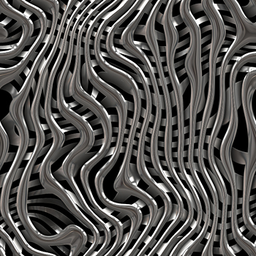
\includegraphics[width=0.5\textwidth]{assets/metal.png}
\end{center}
tiling the image across the entire 480 $\times$ 272 screen using \dcmd{BitmapSize} gives:
\png{tiled-norot}
Which is nice but the repetition is clearly visible.
Rotating the bitmap
using \cmd{rotate}
\cmdidx{cmd\_rotate}
by an odd angle -- 3333 Furmans is about 18$^\circ$ --
makes the repetition much less obvious.

\newpage
\section{Drop shadows}
\index{shadows}
\index{drawing|shadows}
\png{0025}
To give text a drop shadow,
first draw the text in the shadow color, offset by a short distance in both $x$ and $y$.
Then draw the text a second time in the foreground color.
\eg{examples-dropshadow}
This example uses a 3-pixel offset, which works well with a large font.
A smaller font looks better with a 2- or 1-pixel offset.

\noindent
\begin{minipage}[][][t]{0.45\textwidth}

\includegraphics[width=1.0\textwidth]{assets/logodrop.png}
\end{minipage}
\begin{minipage}[][][t]{0.55\textwidth}
A similar technique works for bitmaps: draw the bitmap in black for the shadow, then draw the bitmap
offset by a few pixels.
Here the logo's shadow is lightened by drawing it with 50\% transparency.
\index{logo}
\end{minipage}

\newpage
\section{Fade in and out}

\begin{center}
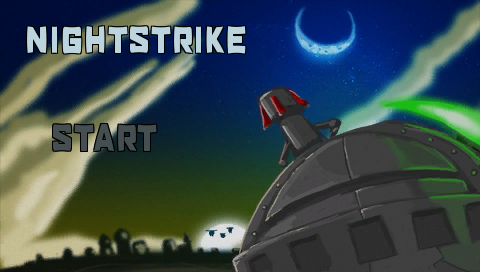
\includegraphics[width=0.3\textwidth]{fade/0.png}
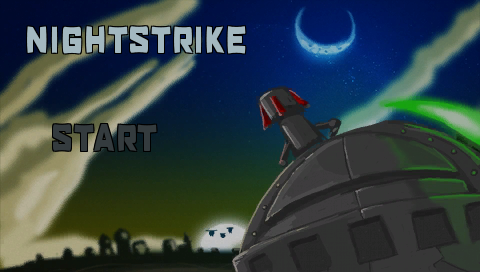
\includegraphics[width=0.3\textwidth]{fade/1.png}
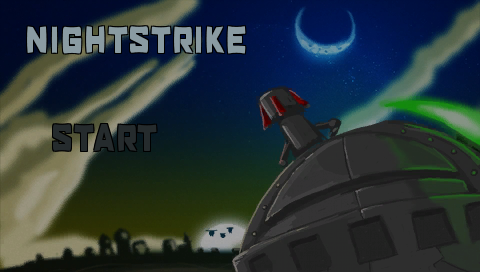
\includegraphics[width=0.3\textwidth]{fade/2.png}
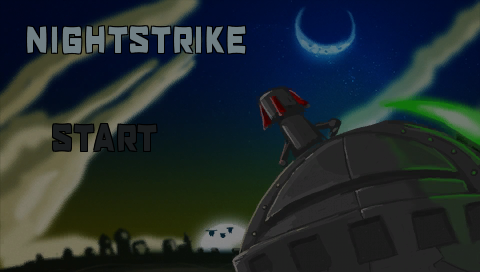
\includegraphics[width=0.3\textwidth]{fade/3.png}
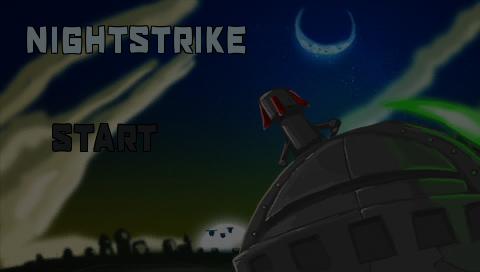
\includegraphics[width=0.3\textwidth]{fade/4.png}
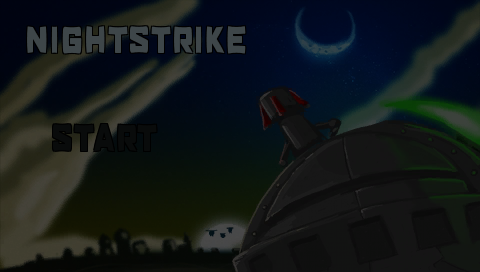
\includegraphics[width=0.3\textwidth]{fade/5.png}
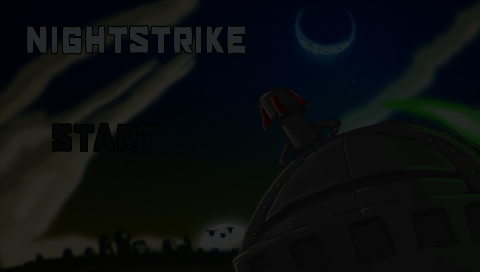
\includegraphics[width=0.3\textwidth]{fade/6.png}
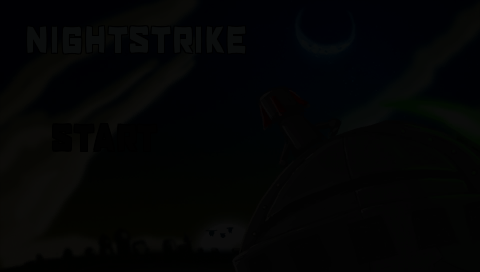
\includegraphics[width=0.3\textwidth]{fade/7.png}
\includegraphics[width=0.3\textwidth]{fade/8.png}
\end{center}

A \term{fade} is when the whole screen gradually turns to one color.
Fades to black and white are most common, but of course any color is possible.
One way of creating a fade is to draw an alpha-blended rectangle covering the whole screen.
The value of the alpha controls how much of the original screen is replaced by the solid rectangle.
By animating alpha from 0 to 255 a fade happens.

Here is \textit{NightStrike}'s code that fades the title screen to black.
\index{NightStrike}

\eg{nightstrike-fade}

Note the \dcmd{TagMask} command, which disables writes
to the tag buffer.
Without this command,
the full-screen rectangle would overwrite all the tag values on the screen.

\newpage
\section{Motion blur}
\index{motion blur}
\index{chess}
\index{demos!chess}
\png{chess}

Motion blur is a graphics technique that smooths out the 
appearance of moving objects, to give a more realistic motion.
The white knight moving in the chess board above is rendered with
motion blur. In freeze-frame the piece looks smeared, but as part of
an animation your eye-brain interprets the blurs as
a fast-moving object.

One way of rendering motion blur on \gdtwo is to draw the object 
multiple times with transparency. In the ``chess'' demo the number of passes
is controlled by \mach{OVERSAMPLE}, which is set to 8.
The renderer makes multiple passes, each time computing a slightly different
position for the piece.  
The eight stacked transparent pieces give a nicely blurred motion along the movement path.

\eg{chess-a}

\newpage
\section{Colors for additive blending}
\index{blending}

\begin{center}
\includegraphics[width=0.55\textwidth]{assets/0048.png}
\includegraphics[width=0.55\textwidth]{assets/0049.png}
\end{center}

Both of these images are drawn by the code below.
The code draws 1000 8-pixel radius circles with a \dcmd{BlendFunc}
set so that each pixel's colors are added to the background's.
The difference is the drawing color: the top image uses a color of pure green
(\mach{0x00ff00})
but the bottom image uses a more subtle greenish shade
(\mach{0x60c030}).

When the color is pure green, any pixels that get drawn more than once simply stay green.
But using the color \mach{0x60c030}
-- which contains a lot of green, some red and a little blue --
means that pixels get brighter each time they are drawn.
A pixel that gets drawn 6 times reaches
\mach{0xffffff},
pure white, and cannot get any brighter.

\eg{examples-additive}

\newpage
\section{Efficient rectangles}
\index{drawing!rectangles}
\png{0052}
The code sets up an \mach{L8} bitmap that is sized 1$\times$1 pixel.
The blend function \mach{(ONE, ZERO)} is a straight replace operation: pixels are copied from the bitmap into the color buffer.
% The source address for the bitmap is set to \mach{ROM\_PIXEL\_FF}, which is an address in the GPU's ROM that has value 255.
For an \mach{L8} bitmap, the RGB pixel values are the current color.

The code sets the bitmap drawn size to 60$\times$30 pixels.
This means that the 60$\times$30 bitmap will be filled with the current color,
so the result is a solid rectangle for each vertex drawn.

Using this method for drawing rectangles differs from 
using \mach{RECTS} in a couple of ways.
Firstly, these rectangles are not anti-aliased: in this example they are exact
60$\times$30 blocks of pixels with no edge smoothing.
The second difference is that here every \dcmd{Vertex2ii} draws one rectangle,
but when drawing with \mach{RECTS} two vertices define each rectangle.
\eg{examples-1x1}

\newpage
\section{1D bitmaps}
\index{bitmaps!1D}
\png{0053}

\eg{examples-1d}

The code uses this 512$\times$1 ``spectrum'' image, loaded into graphics memory as an
\mach{RGB565} bitmap
\begin{center}
\includegraphics[width=1.0\textwidth]{assets/spectrum.png}
\end{center}

\noindent
The \dcmd{BitmapSize} command with \mach{REPEAT}
tiles the bitmap, and since the bitmap height is one pixel, it repeats on every pixel line.
\index{bitmaps!tiling}
% \eg{examples-1d-twist}
As with any bitmap, the 1D bitmap can be rotated and scaled.
Here is the same bitmap scaled by 0.3 and rotated by 80$^\circ$

\begin{center}
\includegraphics[width=0.5\textwidth]{assets/0054.png}
\end{center}

\newpage
\section{Drawing polygons}
\index{drawing!polygons}

\png{0050}

The GD library has a helper object for drawing polygons.
To draw a polygon, first call its
\mach{begin()} method, then supply the vertices of the polygon in order
to the \mach{v()} method, using subpixel coordinates.
Calling \mach{draw()} draws the polygon, using the current color.

This example uses only four vertices, but
a polygon can have up to 16 vertices, and can be any shape.
The vertices do not all need to be on the screen.

The \mach{Poly} object uses a sequence of stencil buffer operations to
compute the outline of the polygon.
It then draws the interior using
the current color and alpha, much like \mach{POINTS} or \mach{LINES} do.

\eg{examples-polygon}

\newpage
Unlike \mach{POINTS} or \mach{LINES}, the polygon's edges are not smoothed --
you can see jagged pixels along the boundary.
One remedy is to outline the polygon with a line.
Here a broad black outline is drawn using
\mach{Poly}'s handy
\mach{outline()} method, which draws the perimeter vertices with
\mach{LINE\_STRIP}

\eg{examples-polygon2}

\png{0051}

\index{demos!cobra}
Using a similar technique, the \textit{cobra} example
first draws all the panels of the spacecraft using
\mach{Poly},
then draws the glowing blue edges.
\index{edges}
\png{cobra}

\newpage
\section{Lines everywhere}
\index{lines}

Because of their round end-caps, wide lines can be used as convenient graphic elements.
The background for the text in the \textit{sprites} demo is a 28 pixel wide line,
drawn in black with about 50\% alpha transparency.
\png{lines-el}
\eg{sprites-line}

\textit{NightStrike} draws the power meter at the top of the screen
\index{NightStrike}
using three horizontal wide lines.
First a 10 pixel wide transparent black line makes a background bar for the power meter.
Two lines draw the power display.
The first is 10 pixels wide in pale orange, the second is 4 pixels wide in bright orange.
Together they give a pleasing glow effect.
\index{glow effect}

\begin{center}
\includegraphics[width=0.28\textwidth]{assets/ns-pwr-0000.png}
\includegraphics[width=0.28\textwidth]{assets/ns-pwr-0001.png}
\includegraphics[width=0.28\textwidth]{assets/ns-pwr-0002.png}
\includegraphics[width=0.28\textwidth]{assets/ns-pwr-0003.png}
\includegraphics[width=0.28\textwidth]{assets/ns-pwr-0004.png}
\includegraphics[width=0.28\textwidth]{assets/ns-pwr-0005.png}
\includegraphics[width=0.28\textwidth]{assets/ns-pwr-0006.png}
\includegraphics[width=0.28\textwidth]{assets/ns-pwr-0007.png}
\includegraphics[width=0.28\textwidth]{assets/ns-pwr-0008.png}
\end{center}

\newpage
\section{Vignette}
\index{photography}

\begin{center}
\includegraphics[width=0.48\textwidth]{assets/vignette-0.png}}
\includegraphics[width=0.48\textwidth]{assets/vignette-1.png}}
\end{center}

In photography,
\term{vignetting} is a darkening
towards the edges of an image.
The image on the right has a vignette applied as an extra layer.
The vignette image itself is a 480$\times$272 \mach{L8} radial gradient,
becoming more opaque towards the edge:

\begin{center}
\setlength{\fboxsep}{0pt}
\setlength{\fboxrule}{1pt}
\fbox{\includegraphics[width=0.6\textwidth]{assets/vignette.png}}
\end{center}

Drawing this bitmap in white will produce a milky transparency towards the edges of the screen.
But drawing this bitmap in black darkens the screen towards the edges.
The amount of darkening can be controlled either by changing the original bitmap, or by 
making the bitmap less opaque with \mach{ColorA}.

\eg{abstract3-vignette}

Because the vignette bitmap does not contain any fine detail, it can be reduced in resolution without
affecting image quality.
A 240$\times$136 vignette bitmap is almost indistinguishable from the 480$\times$272 version, and 
uses one fourth of the memory.

\newpage
\section{Mirroring sprites}
\label{mirror}
\index{bitmaps!mirroring}
\index{sprites}

\noindent
\png{mirror}

\textit{Mirroring} a sprite -- flipping it so that it faces in the opposite direction -- is
very useful in 2D games.
The Gameduino 2's GPU can perform complex bitmap transforms, so a simple flip is no problem at all.
You can think of a left-right flip as a scale by -1 in the $x$ axis, which is done by \cmd{scale}.
The two \cmd{translate} calls adjust the bitmap's position so that the flip happens across the halfway point of the sprite.
In this case, the sprite is 32 pixels wide, so the halfway point is at $x = 16$:

\begin{center}
\begin{tikzpicture}
  \node [opacity=0.4] {\includegraphics[scale=0.32]{previews/walk-WALK-00.png}};
    \draw [dashed,thick]   (0,-1)  -- (0,1);
\end{tikzpicture}
\end{center}

\eg{examples-mirror}

\newpage
\section{Silhouettes and edges}
\index{silhouettes}
\index{drawing!silhouettes}
\index{edges}
\png{outline1}

The Gameduino 2's hardware primitives only draw solid circles and lines.
To draw an edge around a circle -- like the dark slightly transparent edges above --
draw the circle twice.
The first circle is drawn in the edge color and the second, slightly smaller, circle is drawn the with the center color.
For clusters of objects, the drawing order affects the final image.
Here the outlines are all drawn first, which gives a common outline to the whole cluster of circles.

% \eg{abstract3-outline}

\begin{center}
\includegraphics[width=0.48\textwidth]{assets/outline3.png}}
\includegraphics[width=0.48\textwidth]{assets/outline2.png}}
\end{center}

This button graphic is drawn with two wide lines.
The first line is white, and four pixels wider than the blue inner line.
Edges like this can be drawn with
\mach{POINTS},
\mach{LINES} and
\mach{RECTS}.

\begin{center}
\includegraphics[width=0.6\textwidth,trim=120 100 120 100,clip=true]{assets/0057.png}}
\end{center}

\newpage
\section{Chunky pixels}
\cmdidx{cmd\_scale}
\index{retro}
\index{Zardoz}

\png{zardoz}

For the \textit{Zardoz} project by artist and designer Nick Criscuolo, we wanted a
more chunky, 8-bit look from the Gameduino 2's graphics.
So all graphics are drawn at double-size.
At the start of every frame, the game does

\eg{zardoz-double}

\noindent
to double up the size of every bitmap it draws.
The result is that every pixel in the bitmap becomes 2$\times$2 pixels
on the screen.
This makes the effective screen resolution a suitably retro 240$\times$136.
\index{emulating!low resolution displays}

\newpage
\section{Vector graphics}
\index{vector displays}

\png{vector}

\index{drawing!vectors}
Vector graphics games from the 70s, 80s and 90s used special-purpose hardware
to draw bright, colored lines onto a CRT display.
\index{emulating!CRT}
\index{CRT, emulating}
As a graphics technology, the main benefit was a lack of pixels: everything was drawn with
smooth, bright lines and points.
\gdtwo has excellent smooth line and point support, so can easily emulate the vector style of graphics.

However a straight line-drawing game looks a little too `clean'.
The original displays produced a nice glowing look to the lines, which the code below mimics using two passes.
The function \mach{drawgame()} draws the whole of the screen, using \mach{LINES}.
\defidx{LINES}
The first pass draws the background glow for all the lines, so it calls \mach{drawgame()}
with wide, dim lines.
The second pass draws exactly the same screen, but with bright, thin lines.
This two-pass drawing gives an appropriate subtle glow to all the lines.
\index{glow effect}

\eg{tempest-draw}

\newpage
\section{Handmade graphics}
\index{handmade}
\index{weave}
\index{binary}

\begin{center}
\includegraphics[height=0.3\textwidth]{assets/weave.png}}
\includegraphics[height=0.3\textwidth,trim=100 60 100 60,clip=true]{assets/0067.png}}
\end{center}

Early humans didn't have the sophisticated tools we enjoy today.
They had to draw graphics on paper, then turn them into data by hand.
You can still make graphics the same way today.
\cmd{memwrite} writes the 8-byte pattern into memory starting at address zero.
The 1-bit graphic data is coded in \mach{picture[]} -- The ``\mach{0b}'' prefix means binary.
Then it sets up the bitmap parameters, again by hand, for an 8$\times$8 \mach{L1} bitmap, repeating
in $x$ and $y$.

\eg{examples-handmade}

%%%%%%%%%%%%%%%%%%%%%%%%%%%%%%%%%%%%%%%%%%%%%%%%%%%%%%%%%%%%%%%%%%%%%%%%
\chapter{Compositing}

\index{compositing}
This chapter covers some more 
sophisticated graphics techniques that
push the GPU hardware a little further.
They all use compositing -- controlling the color pipeline using the alpha channel.

\newpage
\section{Alpha compositing}

\png{comp1}

\index{drawing!clock}
This stylish clock graphic is drawn using a white circle, a smaller black circle,
then a \cmd{clock} widget to draw the hands.

\eg{examples-comp1}

But adding a JPEG background image gives an unfortunate result

\begin{center}
\includegraphics[width=0.4\textwidth]{assets/comp2.png}
\end{center}
\newpage

The huge black disk spoils the look.
It would be much better to make the central area transparent.
Here is one way of doing that, using the \term{alpha buffer}.

\index{alpha!buffer}
Every pixel on the screen has an alpha value 0-255 that is usually updated at the same time 
as the color buffer.
Normally this alpha buffer is not important, because it is not visible and its contents do not
affect the final image.
But \dcmd{ColorMask} can enable and disable writes to the color and alpha buffers.
This technique ``paints'' the graphic into the alpha buffer, then draws every pixel on the screen
using a blend mode of
\mach{BlendFunc(DST\_ALPHA, ONE)},
which draws the pixels where the alpha buffer is non-zero.

After drawing the tree background image, the first step is to
use \dcmd{ColorMask} to disable color buffer updates,
and set the \dcmd{BlendFunc} to a value that writes incoming alpha
directly into the alpha buffer, by specifying a \term{source blend
factor} of \mach{ONE}:

\eg{examples-comp2a}

Now draw the outer circle just as before

\eg{examples-comp2b}

Nothing appears on the screen yet, because the drawing is only
affecting the alpha buffer, which is -- so far -- invisible.
Drawing the inner circle requires a blend mode that
clears any drawn pixels to zero, so the source blend factor is \mach{ZERO}:

\eg{examples-comp2c}

\newpage
Finally the clock widget itself is drawn, again using a source blend factor of \mach{ONE}:

\eg{examples-comp2d}

After these operations, nothing has been drawn on the visible screen yet --
because the \dcmd{ColorMask} disabled writes to R,G and B.
But the alpha buffer now contains this image:
\begin{center}
\includegraphics[width=0.8\textwidth]{assets/comp1.png}
\end{center}

The final step is to make the alpha buffer visible.
The code does this by drawing a gray rectangle over the entire screen.
Of course, this would simply result in a gray screen,
but the source blend factor is set to \mach{DST\_ALPHA}, so the transparency values come from
the alpha buffer.

\eg{examples-comp2e}
\png{0042}
The complete code is
\eg{examples-comp2}

\newpage
\section{Slot gags}

\begin{center}
\includegraphics[width=0.32\textwidth]{assets/slotgag/00.png}
\includegraphics[width=0.32\textwidth]{assets/slotgag/02.png}
\includegraphics[width=0.32\textwidth]{assets/slotgag/04.png}
\includegraphics[width=0.32\textwidth]{assets/slotgag/06.png}
\includegraphics[width=0.32\textwidth]{assets/slotgag/08.png}
\includegraphics[width=0.32\textwidth]{assets/slotgag/10.png}
\includegraphics[width=0.32\textwidth]{assets/slotgag/12.png}
\includegraphics[width=0.32\textwidth]{assets/slotgag/14.png}
\includegraphics[width=0.32\textwidth]{assets/slotgag/16.png}
\end{center}

\term{Slot gags} are a very old animation technique for 
masking two elements together\footnote{
\index{masking}
See ``Digital Compositing for Film and Video'' by Steve Wright.
}.
In this example of a slot gag, drawing the Gameduino logo bitmap sets the alpha
\index{logo}
buffer to 255 in the logo's pixels, and 0 elsewhere. Then by drawing a wide diagonal line
with \dcmd{BlendFunc} set to \mach{(DST\_ALPHA, ONE)} the line is masked with the alpha buffer,
so only draws pixels where the alpha buffer is 255.
The result is an animated glint effect.
\index{glint effect}
\index{drawing!glint}

\eg{slotgag-a}

\newpage
\section{Patterned text}
\index{drawing!patterned text}
\index{text, patterned}

\png{0060}

Patterned text uses a similar technique to slot gags.
First the text is drawn into the alpha buffer \textit{only}.
Then a full-screen repeating 8$\times$8 bitmap pattern is drawn using the alpha buffer
to control the amount of opacity.

\begin{center}
\includegraphics[width=0.1\textwidth]{previews/examples2-EX2_STRIPE-00.png}
\end{center}
\eg{examples-stripe2}

\newpage
\section{Alpha operators}
\index{alpha}
\png{0063}
You can make alpha-compositing code easier to read 
by using a more expressive name for the blend modes.
Here \mach{PAINT\_ALPHA()} means ``draw something into the alpha buffer''.
\mach{CLEAR\_ALPHA()} means ``erase something from alpha buffer''.

\eg{examples-alpha1}

\newpage
\section{Round-cornered images}
\index{corners, round}
\index{round corners}
\png{0064}

On the left is a 128$\times$128 bitmap drawn using a single \dcmd{Vertex2ii} call.
On the right is the same bitmap drawn using beautiful anti-aliased round corners.
The technique is to draw a round-cornered rectangle into the alpha buffer,
then use this rectangle to control the bitmap transparency, using \dcmd{BlendFunc}.
\index{RECTS}

The corner radius \mach{r} controls how round the corners are, in pixels.
A value of 1 is no rounding, higher values give a more rounded look.
% For batches of round-corners images, for example in a gallery or menu,
% is is a good idea to draw all the rectangles before switching to color buffer drawing
% and rendering the bitmaps themselves.
% This reduces the number of state changes required for each bitmap.

\eg{examples-corners}

\newpage
\section{Transparent buttons}
\png{keypad}
The code first draws a full-screen background image,
then the buttons are each drawn into the alpha buffer by the function \mach{button()}.
Finally, the last six lines make the alpha buffer visible.
\eg{examples-keypad}

\newpage
The \mach{button()} function first paints a white rectangle, then a slightly smaller one with partial transparency.
Lastly it draws the label using \cmd{number}
with \mach{OPT\_CENTER} to center the text.

\eg{examples-button}

\newpage
\section{Reflections}
\index{reflections}
\index{drawing!reflections}
\png{reflection0}

After drawing the top bitmap,
the code draws a 1D vertical 128$\times$1 gradient bitmap into the alpha buffer, repeated horizontally so it covers the screen:

\begin{center}
\includegraphics[width=0.5\textwidth]{assets/reflection1.png}
\end{center}

The code then sets a bitmap transform that flips the logo in the Y axis,
using a method similar to the one in \xref{mirror}.
It then draws the logo's alpha channel into the alpha buffer,
\tern{masked}
with the existing alpha contents.
Masking uses macro \mach{MASK\_ALPHA()}, which multiplies the logo's alpha channel with the existing alpha buffer values:
\index{matte}
\index{masking, alpha}
\index{alpha!masking}

\begin{center}
\vcenter{\hbox{\includegraphics[width=0.3\textwidth]{assets/reflection1.png}}}
$\times$
\vcenter{\hbox{\includegraphics[width=0.3\textwidth]{assets/reflection3.png}}}
$=$
\vcenter{\hbox{\includegraphics[width=0.3\textwidth]{assets/reflection2.png}}}
\end{center}

\newpage
The final step is to draw the mirrored logo using the alpha buffer to control transparency.

\eg{reflection-A}

%%%%%%%%%%%%%%%%%%%%%%%%%%%%%%%%%%%%%%%%%%%%%%%%%%%%%%%%%%%%%%%%%%%%%%%%
\chapter{Saving memory}

\newpage
\section{Two-color images}
\png{mono}
\eg{mono-a}
The source image is this seamless texture, created by Patrick Hoesly
\begin{center}
\includegraphics[width=0.3\textwidth]{assets/tile_green.jpg}
\end{center}
It would be fine to encode this image in
\mach{RGB565} format.
But because it only uses two colors -- and shades in-between --
with some manipulation it can be loaded as an
\mach{L4} bitmap, saving 75\% of the graphics memory.
(See \dcmd{BitmapLayout} for a list of available pixel formats and their memory usage.)

The first step is to load the original image into a graphics program and
measure the two colors, in this case dark green is 
\mach{0x375e03}
and light green is 
\mach{0x68b203}. Then convert the image to monochrome and stretch the contrast
so that it ranges from pure black to pure white
\begin{center}
\includegraphics[width=0.3\textwidth]{assets/tile_greenm.png}
\end{center}

The code first clears the screen to the dark green color,
then draws the \mach{L4} bitmap in light green color.
The result is looks very like the original, but uses much less graphics
memory. This 128 $\times$ 128 bitmap \mach{L4} bitmap uses 8 Kbytes.

As a bonus, you can recolor the bitmap at runtime by adjusting the
foreground and background colors,
\textit{strictly} guided by the rules of good taste, of course.
\begin{center}
\includegraphics[width=0.3\textwidth]{assets/mono1.png}
\includegraphics[width=0.3\textwidth]{assets/mono2.png}
\includegraphics[width=0.3\textwidth]{assets/mono3.png}
\end{center}

\newpage
\section{The missing \mach{L2} format}
\label{twobit}
\index{L2@\mach{L2} bitmap format, emulating}

\png{0055}

Gameduino 2's GPU supports three monochrome formats:
\mach{L1},
\mach{L4} and
\mach{L8}.
The is no \mach{L2} format,
but by drawing in two passes the format can be simulated.
The trick is to split the original 2-bit image into two 1-bit \mach{L1} bitmaps, one for the high bit and one for the low bit:

\begin{center}
\includegraphics[width=0.35\textwidth]{assets/abe1.png}
\includegraphics[width=0.35\textwidth]{assets/abe0.png}
\end{center}

The
\mach{ABE}
graphic is loaded into bitmap handle \mach{ABE\_HANDLE} in cells 0 and 1. Cell 0 contains bit 0, and cell 1 contains bit 1.
The code draws the image in three passes. The first two passes draw the two
bits of the bitmap into the alpha buffer. The third pass makes the alpha buffer visible.

The drawing code first disables color buffer writes using
\dcmd{ColorMask}.
Then it draws the high bit with alpha \mach{0xaa},
and the low bit with \mach{0x55}.
This gives the following values in the alpha buffer for the four 2-bit pixel codes:

\begin{center}
\begin{tabular}{ccc}
high bit & low bit & alpha \\
\hline
0 & 0 & \mach{0x00} \\
0 & 1 & \mach{0x55} \\
1 & 0 & \mach{0xaa} \\
1 & 1 & \mach{0xff} \\
\end{tabular}
\end{center}

\eg{examples-2bit}

The final \dcmd{Vertex2ii} draws the same pixels as the two earlier \dcmd{Vertex2ii} commands.
But because the \dcmd{BlendFunc} is \mach{(DST\_ALPHA, ONE\_MINUS\_DST\_ALPHA)} the bitmap pixels
are ignored -- instead only the contents of the alpha buffer pixels affect the pixel color.

\newpage
\section{Separated mattes}
\index{bitmaps!mattes}
\label{mattes}

\png{nightstrike_1-DEFENSOR_FRONT-00}

The base graphic in
\textit{NightStrike}
\index{NightStrike}
is monochrome with an alpha channel.
There is no direct support in the hardware for a monochrome-with-alpha format, but it
can be emulated by splitting the bitmap into a
\term{matte} -- the original alpha channel -- and a foreground bitmap.

\begin{center}
\includegraphics[width=0.4\textwidth]{previews/nightstrike_1-DEFENSOR_FRONT-00.png}
\includegraphics[width=0.4\textwidth]{previews/nightstrike_1-DEFENSOR_FRONT-01.png}
\end{center}

Both images are loaded as \mach{L4} bitmaps.
The matte bitmap is drawn first, with \dcmd{ColorRGB} set to black.
This clears every pixel covered by the matte.
Then the foreground bitmap is drawn as usual.
\begin{center}
\includegraphics[width=0.3\textwidth]{assets/ns-matteA-0000.png}
\includegraphics[width=0.3\textwidth]{assets/ns-matteB-0000.png}
\end{center}

\newpage
\section{Half-resolution bitmaps}
\index{bitmaps!half-resolution}

For \textit{NightStrike}, the helicopter animation is two frames, 100 pixels wide
\index{NightStrike}
in format \mach{RGBA4}.

\begin{center}
\includegraphics[width=150pt]{previews/nightstrike_1-HELI-00.png}
\includegraphics[width=150pt]{previews/nightstrike_1-HELI-01.png}
\end{center}

There is another four frame animation, used when the stricken helicopter is crashing to the ground.
Because this animation is seen only briefly, when the sprite is moving fast,
a loss of detail is not too noticable.
This version is half the resolution, less than 50 pixels wide, but is scaled by \cmd{scale} so that it
appears 100 pixels wide on the screen.
Halving the resolution of a bitmap reduces its memory usage by 75\%.

\begin{center}
\includegraphics[width=135pt]{previews/nightstrike_1-COPTER_FALL-00.png}
\includegraphics[width=135pt]{previews/nightstrike_1-COPTER_FALL-01.png}
\includegraphics[width=135pt]{previews/nightstrike_1-COPTER_FALL-02.png}
\includegraphics[width=135pt]{previews/nightstrike_1-COPTER_FALL-03.png}
\end{center}

\newpage
\section{8-bit formats}
\label{eightbit}

\begin{center}
\includegraphics[width=0.6\textwidth]{assets/0034.png}
\end{center}

For most images, the 16-bit per pixels formats --
\mach{RGB565},
\mach{ARGB1555} and
\mach{ARGB4} -- 
are appropriate. But sometimes the 8-bit per pixel formats can be used instead with little noticable loss in quality.

The playing cards above are encoded in
\mach{RGB332} format, so only use one byte per pixel. The explosion animation below uses
\mach{ARGB2} format.
\index{playing cards}
\index{cards}
The playing cards use bold colors, so the reduced color range of \mach{RGB332} is not very noticable.
The explosion animates very fast -- the whole sequence below takes 1/4th of a second --
and this rapid motion conceals the reduced color range.
\index{explosion}
\index{animation}

\begin{center}
\includegraphics[width=0.19\textwidth]{previews/nightstrike_1-FIRE-00.png}
\includegraphics[width=0.19\textwidth]{previews/nightstrike_1-FIRE-01.png}
\includegraphics[width=0.19\textwidth]{previews/nightstrike_1-FIRE-02.png}
\includegraphics[width=0.19\textwidth]{previews/nightstrike_1-FIRE-03.png}
\includegraphics[width=0.19\textwidth]{previews/nightstrike_1-FIRE-04.png}
\includegraphics[width=0.19\textwidth]{previews/nightstrike_1-FIRE-05.png}
\includegraphics[width=0.19\textwidth]{previews/nightstrike_1-FIRE-06.png}
\includegraphics[width=0.19\textwidth]{previews/nightstrike_1-FIRE-07.png}
\includegraphics[width=0.19\textwidth]{previews/nightstrike_1-FIRE-08.png}
\includegraphics[width=0.19\textwidth]{previews/nightstrike_1-FIRE-09.png}
\includegraphics[width=0.19\textwidth]{previews/nightstrike_1-FIRE-10.png}
\includegraphics[width=0.19\textwidth]{previews/nightstrike_1-FIRE-11.png}
\includegraphics[width=0.19\textwidth]{previews/nightstrike_1-FIRE-12.png}
\includegraphics[width=0.19\textwidth]{previews/nightstrike_1-FIRE-13.png}
\includegraphics[width=0.19\textwidth]{previews/nightstrike_1-FIRE-14.png}
\end{center}
\clearpage

\newpage
\section{DXT1}
\label{dxt1}
\index{DXT1}

\begin{center}
\includegraphics[width=0.48\textwidth]{assets/nightstrike/backgrounds/welcome.jpg}
\includegraphics[width=0.48\textwidth]{assets/dxt1.png}
\end{center}

DXT is a texture compression system -- it squeezes a bigger image into less graphics memory.
The image on the left is the artist's original rendering of the \textit{NightStrike} welcome screen. On the right is a screenshot
from the DXT1-compressed version on the running \gdtwo. As you can see, the differences are quite small.
But because it uses DXT1,
the image on the right uses \textit{one fourth} of the graphics memory of the image on the left.

Roughly, DXT1 works by splitting the image into 4$\times$4 pixel tiles. Each tile is given two colors, call them
$C_0$ and $C_1$. Then each pixel in the tile is specified only as a mixture of $C_0$ and $C_1$.
DXT1 uses \mach{RGB565} format for the colors $C_0$ and $C_1$, and for each pixel it uses a two bit code:

\vspace{10pt}
\begin{tabular}{cl}
code & final color \\
\hline \\
00 & $C_0$ \\
01 & $0.666 \times C_0 + 0.333 \times C_1$ \\
10 & $0.333 \times C_0 + 0.666 \times C_1$ \\
11 & $C_1$ \\
\end{tabular}
\vspace{10pt}

\noindent
so the storage for each 4$\times$4 tile, in bits, is:

\vspace{10pt}
\begin{tabular}{cl}
$C_0$ & 16 \\
$C_1$ & 16 \\
pixels & 16 $\times$ 2 = 32 \\
\end{tabular}
\vspace{10pt}

Each tile uses 64 bits, and there are sixteen pixels in each tile, so the \textit{per pixel}
storage is only 4 bits. If the bitmap were encoded in plain \mach{RGB565} it would need 16 bits per pixel,
so the graphics memory saving is 75\%!

\gdtwo's graphics hardware does not directly support DXT1, but by using multiple drawing passes and multiple bitmaps, it can
simulate the DXT1 format.

\clearpage

Taking the \textit{NightStrike} welcome screen as an example, the source image is 480$\times$272 pixels.
Hence the width in 4$\times$4 tiles is 120$\times$68. So the $C_0$ and $C_1$ images are both encoded in \mach{RGB565} at a resolution of
120$\times$68:

\begin{center}
$C_0=$
\vcenter{\hbox{\includegraphics[width=0.9\textwidth]{previews/nightstrike_welcome-WELCOME_BACKGROUND_COLOR-00.png}}}
\end{center}

\begin{center}
$C_1=$
\vcenter{\hbox{\includegraphics[width=0.9\textwidth]{previews/nightstrike_welcome-WELCOME_BACKGROUND_COLOR-01.png}}}
\end{center}

Because the hardware does not directly support 2-bit bitmaps, the two bit layer is split into two 1-bit images,
using the same technique as \xref{twobit}. 

\begin{center}
$b_0=$
\vcenter{\hbox{\includegraphics[width=0.32\textwidth]{previews/nightstrike_welcome-WELCOME_BACKGROUND_BITS-00.png}}}
$\;\;\;\;\;\;b_1=$
\vcenter{\hbox{\includegraphics[width=0.32\textwidth]{previews/nightstrike_welcome-WELCOME_BACKGROUND_BITS-01.png}}}
\end{center}
\vspace{10pt}

\noindent
\textit{NightStrike's} DXT1 background drawing function first builds the 2-bit image in the alpha buffer.
It then
writes the $C_0$ and $C_1$ bitmaps (zoomed 4$\times$ using \cmd{scale}) into the color buffer, with the blend values from the alpha buffer.

\eg{nightstrike-dxt1}

%%%%%%%%%%%%%%%%%%%%%%%%%%%%%%%%%%%%%%%%%%%%%%%%%%%%%%%%%%%%%%%%%%%%%%%%
% \chapter{Useful things}
% \section{Light switch}
% \section{Kitchen timer}
% \section{Photo frame}

\chapter{Games and demos}

\newpage
\section{Kenney}

\png{kenney}

The \textit{kenney} demo uses public domain artwork\footnote{\url{http://opengameart.org/content/platformer-art-deluxe}}
by artist Kenney.nl
\footnote{\url{http://www.kenney.nl/}}
.
It draws six scrolling layers,
and runs smoothly at 60Hz.
Most layers are drawn using bitmaps, all encoded with format \mach{ARGB4}.
The first layer is a vertical gradient, with carefully chosen sky-blue colors.

\png{kenney_0}
\eg{kenney-gradient}

\noindent
The next layer uses a single sprite loaded in \mach{CLOUD\_HANDLE}
drawn in the random positions in \mach{state.clouds[]}.
The clouds all move downwards at slightly different rates,
and slower-moving clouds are more transparent.
As clouds reach the bottom of the screen, they wrap around to the top.
The clouds' positions are subpixel coordinates, in 1/16th of a pixel.
This extra precision means that as the clouds move, they don't ``snap''
between integer pixel coordinates.

\szpng{0.2}{previews/kenney-CLOUD-00}
\png{kenney_1}
\eg{kenney-clouds}


% \szpng{0.15}{kenney_tiles}
\sbs{kenney_tiles}{
The next layer is the tile map.
The tile map was created using the ``tiled''
editor (\url{http://www.mapeditor.org/}), and imported 
using the asset converter into character array 
\mach{layer1\_map}.
The 20 tiles are each 32$\times$32 bitmaps, encoded as \mach{ARGB4}
in handle \mach{TILES\_HANDLE}.
Tile code zero is the blank cell, and the code checks for this and only
draws tiles with non-zero codes.
\szpng{1.0}{kenney_2}
}
\begin{center}
\includegraphics[width=0.09\textwidth]{previews/kenney-TILES-00.png}
\includegraphics[width=0.09\textwidth]{previews/kenney-TILES-01.png}
\includegraphics[width=0.09\textwidth]{previews/kenney-TILES-02.png}
\includegraphics[width=0.09\textwidth]{previews/kenney-TILES-03.png}
\includegraphics[width=0.09\textwidth]{previews/kenney-TILES-04.png}
\includegraphics[width=0.09\textwidth]{previews/kenney-TILES-05.png}
\includegraphics[width=0.09\textwidth]{previews/kenney-TILES-06.png}
\includegraphics[width=0.09\textwidth]{previews/kenney-TILES-07.png}
\includegraphics[width=0.09\textwidth]{previews/kenney-TILES-08.png}
\includegraphics[width=0.09\textwidth]{previews/kenney-TILES-09.png}
\includegraphics[width=0.09\textwidth]{previews/kenney-TILES-10.png}
\includegraphics[width=0.09\textwidth]{previews/kenney-TILES-11.png}
\includegraphics[width=0.09\textwidth]{previews/kenney-TILES-12.png}
\includegraphics[width=0.09\textwidth]{previews/kenney-TILES-13.png}
\includegraphics[width=0.09\textwidth]{previews/kenney-TILES-14.png}
\includegraphics[width=0.09\textwidth]{previews/kenney-TILES-15.png}
\includegraphics[width=0.09\textwidth]{previews/kenney-TILES-16.png}
\includegraphics[width=0.09\textwidth]{previews/kenney-TILES-17.png}
\includegraphics[width=0.09\textwidth]{previews/kenney-TILES-18.png}
\includegraphics[width=0.09\textwidth]{previews/kenney-TILES-19.png}
\end{center}
\eg{kenney-tiles}

\newpage
The foreground characters are \mach{ARGB4} bitmaps, rotated at random
and following gentle sinusoidal paths.
Their coordinates are in \mach{state.p}.
\begin{center}
\includegraphics[width=0.2\textwidth]{previews/kenney-PLAYER1-00.png}
\includegraphics[width=0.2\textwidth]{previews/kenney-PLAYER1-01.png}
\includegraphics[width=0.2\textwidth]{previews/kenney-PLAYER1-02.png}
\end{center}
The trails of colored ``bubbles'' following each character are transparent
\mach{POINT}s, handled in the code by three \mach{state.trail} objects.
\png{kenney_3}
\eg{kenney-player}

The ``sunburst'' graphic is drawn between the sky and cloud layers.
It uses a series of stencil operations to create the ray objects.
The function \mach{burst()} draws a complete sunburst, and
\mach{sunrise()} draws both the orange and yellow \mach{burst()}s, and animates their bouncing expansion.

\png{kenney_4}

The final layer is the shower of hearts falling down the screen.
These are handled like the ``cloud'' layer.
Array \mach{state.hearts[]} tracks their position, and they move downwards, wrapping around from bottom to top.
\szpng{0.2}{previews/kenney-HEART-00}

\png{kenney_5}

\newpage
\section{NightStrike}
\label{nightstrike}
\index{NightStrike|boldindex}

\png{nightstrike}

The \textit{NightStrike} game uses public domain artwork
\footnote{\url{http://opengameart.org/content/nightstrike-png-assets}}
by artist MindChamber.
It uses the touch screen to track dozens of independent objects,
and plays smoothly at 60Hz.
The game uses some special techniques to fit its graphics into the available 256 KBytes of memory.

The game has five levels, and each level is a separate asset file, containing all the background and foreground graphics
for the level, as well as sound effects.
The backgrounds for each level are 480$\times$272 images, encoded using DXT1-like compression
(see \xref{dxt1})
so they only use 65 Kbytes of video memory.

\begin{center}
\includegraphics[width=0.3\textwidth]{assets/nightstrike/backgrounds/welcome.jpg}
\includegraphics[width=0.3\textwidth]{assets/nightstrike/backgrounds/burningwoods.jpg}
\includegraphics[width=0.3\textwidth]{assets/nightstrike/backgrounds/greenland.jpg}
\includegraphics[width=0.3\textwidth]{assets/nightstrike/backgrounds/nightfall.jpg}
\includegraphics[width=0.3\textwidth]{assets/nightstrike/backgrounds/purplesnow.jpg}
\includegraphics[width=0.3\textwidth]{assets/nightstrike/backgrounds/redworld.jpg}
\end{center}

\newpage

The sprites in the game have smooth transparency, so most are encoded in \mach{ARGB4} format.

\begin{center}
\includegraphics[width=150pt]{previews/nightstrike_1-HELI-00.png}
\includegraphics[width=150pt]{previews/nightstrike_1-HELI-01.png}
\end{center}

\begin{center}
\includegraphics[width=0.07\textwidth]{previews/nightstrike_0-MISSILE_A-00.png}
\includegraphics[width=0.07\textwidth]{previews/nightstrike_0-MISSILE_C-00.png}
\end{center}

\begin{center}
\includegraphics[width=0.1\textwidth]{previews/nightstrike_0-SOLDIER_RUN-00.png}
\includegraphics[width=0.1\textwidth]{previews/nightstrike_0-SOLDIER_RUN-01.png}
\includegraphics[width=0.1\textwidth]{previews/nightstrike_0-SOLDIER_RUN-02.png}
\includegraphics[width=0.1\textwidth]{previews/nightstrike_0-SOLDIER_RUN-03.png}
\includegraphics[width=0.1\textwidth]{previews/nightstrike_0-SOLDIER_RUN-04.png}
\includegraphics[width=0.1\textwidth]{previews/nightstrike_0-SOLDIER_RUN-05.png}
\includegraphics[width=0.1\textwidth]{previews/nightstrike_0-SOLDIER_RUN-06.png}
\includegraphics[width=0.1\textwidth]{previews/nightstrike_0-SOLDIER_RUN-07.png}
\end{center}

The explosions in the game animate quickly and have bright colors, so can
use \mach{ARGB2} format to save memory (see \xref{eightbit}).

\begin{center}
\includegraphics[width=0.18\textwidth]{previews/nightstrike_0-EXPLODE_BIG-00.png}
\includegraphics[width=0.18\textwidth]{previews/nightstrike_0-EXPLODE_BIG-01.png}
\includegraphics[width=0.18\textwidth]{previews/nightstrike_0-EXPLODE_BIG-02.png}
\includegraphics[width=0.18\textwidth]{previews/nightstrike_0-EXPLODE_BIG-03.png}
\includegraphics[width=0.18\textwidth]{previews/nightstrike_0-EXPLODE_BIG-04.png}
\includegraphics[width=0.18\textwidth]{previews/nightstrike_0-EXPLODE_BIG-05.png}
\includegraphics[width=0.18\textwidth]{previews/nightstrike_0-EXPLODE_BIG-06.png}
\includegraphics[width=0.18\textwidth]{previews/nightstrike_0-EXPLODE_BIG-07.png}
\includegraphics[width=0.18\textwidth]{previews/nightstrike_0-EXPLODE_BIG-08.png}
\includegraphics[width=0.18\textwidth]{previews/nightstrike_0-EXPLODE_BIG-09.png}
\end{center}

The player's ``defensor'' is monochrome, so it is drawn using two \mach{L4} bitmaps (see \xref{mattes}).

\begin{center}
\includegraphics[width=0.4\textwidth]{previews/nightstrike_1-DEFENSOR_FRONT-00.png}
\includegraphics[width=0.4\textwidth]{previews/nightstrike_1-DEFENSOR_FRONT-01.png}
\end{center}

\newpage

As well as using animated bitmaps for explosions,
the game draws exploding sparks using wide lines (see \xref{lines}).
Because they use \mach{LINES}, the sparks require no graphics memory
\begin{center}
\includegraphics[width=0.3\textwidth]{assets/ns-lines-0006.png}
\includegraphics[width=0.3\textwidth]{assets/ns-lines-0007.png}
\includegraphics[width=0.3\textwidth]{assets/ns-lines-0008.png}
\includegraphics[width=0.3\textwidth]{assets/ns-lines-0009.png}
\includegraphics[width=0.3\textwidth]{assets/ns-lines-0010.png}
\includegraphics[width=0.3\textwidth]{assets/ns-lines-0011.png}
\end{center}

\noindent
In game text uses a small 12$\times$19 pixel font, converted from an
original TrueType font.
This font's bitmaps are in \mach{L4} format, to preserve its smooth edges.

\begin{center}
\includegraphics[width=0.04\textwidth]{previews/nightstrike_2-INFOFONT-00.png}
\includegraphics[width=0.04\textwidth]{previews/nightstrike_2-INFOFONT-01.png}
\includegraphics[width=0.04\textwidth]{previews/nightstrike_2-INFOFONT-02.png}
\includegraphics[width=0.04\textwidth]{previews/nightstrike_2-INFOFONT-03.png}
\includegraphics[width=0.04\textwidth]{previews/nightstrike_2-INFOFONT-04.png}
\includegraphics[width=0.04\textwidth]{previews/nightstrike_2-INFOFONT-05.png}
\includegraphics[width=0.04\textwidth]{previews/nightstrike_2-INFOFONT-06.png}
\includegraphics[width=0.04\textwidth]{previews/nightstrike_2-INFOFONT-07.png}
\includegraphics[width=0.04\textwidth]{previews/nightstrike_2-INFOFONT-10.png}
\includegraphics[width=0.04\textwidth]{previews/nightstrike_2-INFOFONT-11.png}
\includegraphics[width=0.04\textwidth]{previews/nightstrike_2-INFOFONT-12.png}
\includegraphics[width=0.04\textwidth]{previews/nightstrike_2-INFOFONT-13.png}
\includegraphics[width=0.04\textwidth]{previews/nightstrike_2-INFOFONT-14.png}
\includegraphics[width=0.04\textwidth]{previews/nightstrike_2-INFOFONT-15.png}
\includegraphics[width=0.04\textwidth]{previews/nightstrike_2-INFOFONT-16.png}
\includegraphics[width=0.04\textwidth]{previews/nightstrike_2-INFOFONT-17.png}
\includegraphics[width=0.04\textwidth]{previews/nightstrike_2-INFOFONT-20.png}
\includegraphics[width=0.04\textwidth]{previews/nightstrike_2-INFOFONT-21.png}
\includegraphics[width=0.04\textwidth]{previews/nightstrike_2-INFOFONT-22.png}
\includegraphics[width=0.04\textwidth]{previews/nightstrike_2-INFOFONT-23.png}
\includegraphics[width=0.04\textwidth]{previews/nightstrike_2-INFOFONT-24.png}
\includegraphics[width=0.04\textwidth]{previews/nightstrike_2-INFOFONT-25.png}
\includegraphics[width=0.04\textwidth]{previews/nightstrike_2-INFOFONT-26.png}
\includegraphics[width=0.04\textwidth]{previews/nightstrike_2-INFOFONT-27.png}
\includegraphics[width=0.04\textwidth]{previews/nightstrike_2-INFOFONT-28.png}
\includegraphics[width=0.04\textwidth]{previews/nightstrike_2-INFOFONT-29.png}
\includegraphics[width=0.04\textwidth]{previews/nightstrike_2-INFOFONT-30.png}
\includegraphics[width=0.04\textwidth]{previews/nightstrike_2-INFOFONT-31.png}
\includegraphics[width=0.04\textwidth]{previews/nightstrike_2-INFOFONT-32.png}
\includegraphics[width=0.04\textwidth]{previews/nightstrike_2-INFOFONT-33.png}
\includegraphics[width=0.04\textwidth]{previews/nightstrike_2-INFOFONT-34.png}
\includegraphics[width=0.04\textwidth]{previews/nightstrike_2-INFOFONT-35.png}
\includegraphics[width=0.04\textwidth]{previews/nightstrike_2-INFOFONT-36.png}
\includegraphics[width=0.04\textwidth]{previews/nightstrike_2-INFOFONT-37.png}
\includegraphics[width=0.04\textwidth]{previews/nightstrike_2-INFOFONT-38.png}
\includegraphics[width=0.04\textwidth]{previews/nightstrike_2-INFOFONT-39.png}
\includegraphics[width=0.04\textwidth]{previews/nightstrike_2-INFOFONT-40.png}
\includegraphics[width=0.04\textwidth]{previews/nightstrike_2-INFOFONT-41.png}
\includegraphics[width=0.04\textwidth]{previews/nightstrike_2-INFOFONT-42.png}
\includegraphics[width=0.04\textwidth]{previews/nightstrike_2-INFOFONT-43.png}
\includegraphics[width=0.04\textwidth]{previews/nightstrike_2-INFOFONT-44.png}
\includegraphics[width=0.04\textwidth]{previews/nightstrike_2-INFOFONT-45.png}
\includegraphics[width=0.04\textwidth]{previews/nightstrike_2-INFOFONT-46.png}
\includegraphics[width=0.04\textwidth]{previews/nightstrike_2-INFOFONT-47.png}
\includegraphics[width=0.04\textwidth]{previews/nightstrike_2-INFOFONT-48.png}
\includegraphics[width=0.04\textwidth]{previews/nightstrike_2-INFOFONT-49.png}
\includegraphics[width=0.04\textwidth]{previews/nightstrike_2-INFOFONT-50.png}
\includegraphics[width=0.04\textwidth]{previews/nightstrike_2-INFOFONT-51.png}
\includegraphics[width=0.04\textwidth]{previews/nightstrike_2-INFOFONT-52.png}
\includegraphics[width=0.04\textwidth]{previews/nightstrike_2-INFOFONT-53.png}
\includegraphics[width=0.04\textwidth]{previews/nightstrike_2-INFOFONT-54.png}
\includegraphics[width=0.04\textwidth]{previews/nightstrike_2-INFOFONT-55.png}
\includegraphics[width=0.04\textwidth]{previews/nightstrike_2-INFOFONT-56.png}
\includegraphics[width=0.04\textwidth]{previews/nightstrike_2-INFOFONT-57.png}
\includegraphics[width=0.04\textwidth]{previews/nightstrike_2-INFOFONT-58.png}
\includegraphics[width=0.04\textwidth]{previews/nightstrike_2-INFOFONT-59.png}
\includegraphics[width=0.04\textwidth]{previews/nightstrike_2-INFOFONT-60.png}
\includegraphics[width=0.04\textwidth]{previews/nightstrike_2-INFOFONT-61.png}
\includegraphics[width=0.04\textwidth]{previews/nightstrike_2-INFOFONT-62.png}
\includegraphics[width=0.04\textwidth]{previews/nightstrike_2-INFOFONT-63.png}
\includegraphics[width=0.04\textwidth]{previews/nightstrike_2-INFOFONT-64.png}
\includegraphics[width=0.04\textwidth]{previews/nightstrike_2-INFOFONT-65.png}
\includegraphics[width=0.04\textwidth]{previews/nightstrike_2-INFOFONT-66.png}
\includegraphics[width=0.04\textwidth]{previews/nightstrike_2-INFOFONT-67.png}
\includegraphics[width=0.04\textwidth]{previews/nightstrike_2-INFOFONT-68.png}
\includegraphics[width=0.04\textwidth]{previews/nightstrike_2-INFOFONT-69.png}
\includegraphics[width=0.04\textwidth]{previews/nightstrike_2-INFOFONT-70.png}
\includegraphics[width=0.04\textwidth]{previews/nightstrike_2-INFOFONT-71.png}
\includegraphics[width=0.04\textwidth]{previews/nightstrike_2-INFOFONT-72.png}
\includegraphics[width=0.04\textwidth]{previews/nightstrike_2-INFOFONT-73.png}
\includegraphics[width=0.04\textwidth]{previews/nightstrike_2-INFOFONT-74.png}
\includegraphics[width=0.04\textwidth]{previews/nightstrike_2-INFOFONT-75.png}
\includegraphics[width=0.04\textwidth]{previews/nightstrike_2-INFOFONT-76.png}
\includegraphics[width=0.04\textwidth]{previews/nightstrike_2-INFOFONT-77.png}
\includegraphics[width=0.04\textwidth]{previews/nightstrike_2-INFOFONT-78.png}
\includegraphics[width=0.04\textwidth]{previews/nightstrike_2-INFOFONT-79.png}
\includegraphics[width=0.04\textwidth]{previews/nightstrike_2-INFOFONT-80.png}
\includegraphics[width=0.04\textwidth]{previews/nightstrike_2-INFOFONT-81.png}
\includegraphics[width=0.04\textwidth]{previews/nightstrike_2-INFOFONT-82.png}
\includegraphics[width=0.04\textwidth]{previews/nightstrike_2-INFOFONT-83.png}
\includegraphics[width=0.04\textwidth]{previews/nightstrike_2-INFOFONT-84.png}
\includegraphics[width=0.04\textwidth]{previews/nightstrike_2-INFOFONT-85.png}
\includegraphics[width=0.04\textwidth]{previews/nightstrike_2-INFOFONT-86.png}
\includegraphics[width=0.04\textwidth]{previews/nightstrike_2-INFOFONT-87.png}
\includegraphics[width=0.04\textwidth]{previews/nightstrike_2-INFOFONT-88.png}
\includegraphics[width=0.04\textwidth]{previews/nightstrike_2-INFOFONT-89.png}
\includegraphics[width=0.04\textwidth]{previews/nightstrike_2-INFOFONT-90.png}
\includegraphics[width=0.04\textwidth]{previews/nightstrike_2-INFOFONT-91.png}
\includegraphics[width=0.04\textwidth]{previews/nightstrike_2-INFOFONT-92.png}
\includegraphics[width=0.04\textwidth]{previews/nightstrike_2-INFOFONT-93.png}
\includegraphics[width=0.04\textwidth]{previews/nightstrike_2-INFOFONT-94.png}
\end{center}

The game code uses a class for each kind of visble object in the game.
These class are:
\mach{Fires},
\mach{Explosions},
\mach{Sparks},
\mach{SoldierObject},
\mach{MissileObject}, \\
\mach{Rewards},
\mach{BaseObject}, and
\mach{HeliObject}.
Each object has a \mach{draw()} method to draw the object on the screen,
and an \mach{update()} method to animate, move and compute any collisions.
Object collision testing uses a simple overlapping box scheme.

\testit{NightStrike} uses 20 Kbytes of the Arduino's 32 Kbytes of flash, and
the game loop runs in about 7ms on a standard 16MHz Arduino.

\newpage
\section{Invaders}

\png{invaders}

\textit{Invaders} is a port of the original Gameduino game \footnote{
\url{http://artlum.com/gameduino/gameduino.html}}.
But to make it more authentic, it includes the original arcade cabinet artwork.
The original `70s arcade cabinet only had a monochrome CRT screen,
but to jazz it up the designers used a cunning mirror arrangement to project a suitable
space picture behind the graphics.
If you look closely you can see that the pixels are slightly transparent because of this.
Their other trick was to put a colored overlay on the CRT screen with a green band at the bottom and a red one at the top.
In the original game you can see the missiles and bombs change color as they pass through the colored zones.

\gdtwo \textit{invaders} loads the background image as a 248$\times$272 JPEG.
Because it only uses 6K it fits easily in the Arduino's flash memory.
% The background image itself is \term{contrast stretched} - it uses the full range
% of colors from black to white.
% Doing this means that the image compresses well in JPEG and also 
Encoding the full-brightness image then drawing a darker version in the game helps to
conceal some of the JPEG compression artefacts in the sky gradient.

The game's pixel action is drawn into the alpha buffer.
To make it visible, the 28$\times$32 overlay bitmap
is drawn zoomed 8X so that its size is 248$\times$256,
with \dcmd{BlendFunc} \mach{(DST\_ALPHA, ONE\_MINUS\_DST\_ALPHA)}.
This paints the game's pixels, using the color from the overlay.

\newpage
\begin{center}
\includegraphics[width=0.6\textwidth]{assets/invaders-272.png}
\end{center}

\begin{center}
\begin{tikzpicture}[scale=0.02142857142857143]
\node[anchor=south west,inner sep=0] (image) at (0,0) {\includegraphics[width=0.6\textwidth]{assets/invaders-overlay.png}};
\foreach \x in {0,...,28}
  \draw [lightgray] (\x\textwidth,0) -- (\x\textwidth,32\textwidth);
\foreach \y in {0,...,32}
  \draw [lightgray] (0,\y\textwidth) -- (28\textwidth,\y\textwidth);
\end{tikzpicture}
\end{center}

% \section{Zardoz}

\appendix
\chapter{The asset converter}

The latest \gdtwo asset converter is available at

\url{http://gameduino.com/code}

\noindent
Detailed documentation is available online.

\clearpage
\addcontentsline{toc}{chapter}{Index}
\printindex

\end{document}

% DONE:
%   Continuous playback
%   Font loading
%   Vertex2f
%   SDcard
%   {Blending} useful modes
%   Invaders
%   Kenney
%   NightStrike
%   Accelerometer
%   Plug in...
%
% TODO:
%   Streamer
%   Poly
